\documentclass[a4paper,11pt,openany]{book}

\usepackage[T1]{fontenc}
\usepackage[utf8]{inputenc}
\usepackage[italian]{babel}
\usepackage[top=2cm,bottom=2cm,left=2cm,right=2cm]{geometry}
\usepackage{indentfirst}
\usepackage{parskip}
%--------------------------------------------------------------------------------------------------------------
\usepackage{amssymb,amsmath,amsthm,amsfonts}
%--------------------------------------------------------------------------------------------------------------
\usepackage{graphicx}
%\usepackage{subfigure}
\usepackage{subcaption}
%--------------------------------------------------------------------------------------------------------------
\usepackage{tabularx}
\usepackage{multirow}
%--------------------------------------------------------------------------------------------------------------
\usepackage{hyperref}
%--------------------------------------------------------------------------------------------------------------
\usepackage{mhchem}
%--------------------------------------------------------------------------------------------------------------
\usepackage{xspace}
\usepackage[font=small]{caption}
\usepackage{eucal}
\usepackage{eso-pic}
\usepackage{booktabs}
\usepackage{afterpage}
\usepackage{fancyhdr}
\usepackage{textcomp}
\usepackage{setspace}
\usepackage[a-3u]{pdfx}
\pagestyle{fancy} 
%--------------------------------------------------------------------------------------------------------------
\usepackage[backend=biber, style=numeric, sorting=none, maxbibnames=99, minbibnames=99]{biblatex}
\addbibresource{bibliography.bib}
%--------------------------------------------------------------------------------------------------------------
% Definiamo il nuovo tipo "schema"
% Sintassi: \DeclareCaptionType{nome_ambiente}[Etichetta_Didascalia][Titolo_Indice]
\DeclareCaptionType{schema}[Schema][Elenco degli Schemi]
%------------------------------------------------------------------------------------------------------------------------------------------------------------------------
\usepackage[most]{tcolorbox}

\usepackage{listings}
\usepackage{xcolor}

% --- Custom Colors for Python Syntax Highlighting ---
\definecolor{pybackground}{RGB}{248, 248, 248}  % Soft light gray
\definecolor{pyborder}{RGB}{80, 80, 80}         % Kinda black / dark gray
\definecolor{pycomments}{RGB}{63, 127, 95}      % Classic green for comments
\definecolor{pykeywords}{RGB}{0, 0, 225}        % Python blue for keywords
\definecolor{pystrings}{RGB}{186, 33, 33}       % Dark red for strings
\definecolor{pynumbers}{RGB}{120, 120, 120}     % Medium gray for line numbers
\definecolor{pybuiltins}{RGB}{0, 130, 0}        % Green for built-in functions (print, len, etc.)

% --- Global Listings Setup ---
\lstset{
    language=Python,
    backgroundcolor=\color{pybackground},
    % --- Width and Centering ---
    linewidth=0.85\textwidth,               % Makes the block 85% of text width
    xleftmargin=0.075\textwidth,            % Centers the block (100% - 85% = 15% remaining / 2 = 7.5%)
    % --- Border and Framing ---
    frame=single,                           % Single frame border around the code
    rulecolor=\color{pyborder},             % Color of the border
    frameround=ffff,                        % Square corners (change to tttt for round)
    % --- Typography ---
    basicstyle=\ttfamily\small,             % Monospace font for code
    keywordstyle=\color{pykeywords}\bfseries,
    commentstyle=\color{pycomments}\itshape,
    stringstyle=\color{pystrings},
    morekeywords={as, assert, break, class, continue, def, del, elif, else, except, False, finally, for, from, global, if, import, in, is, lambda, None, nonlocal, not, or, pass, raise, return, True, try, while, with, yield}, % Ensure all modern keywords are caught
    % --- Line Numbers ---
    numbers=left,                           % Line numbers on the left
    numberstyle=\tiny\color{pynumbers},     % Style and color of line numbers
    numbersep=10pt,                         % Distance between numbers and code
    % --- Whitespace and Formatting ---
    breaklines=true,                        % Automatically wrap long lines
    breakatwhitespace=false,                % Wrap lines anywhere, not just at spaces
    showstringspaces=false,                 % Don't show ugly visual indicators for spaces in strings
    keepspaces=true,                        % Keeps alignment spaces intact
    columns=flexible                        % Better character spacing
}
%-----------------------------------------------------------------------------------------------------------------------------------------------------------------------------------------




\begin{document}
    
\frontmatter %----------------------------------------------------------------------
\begin{titlepage}

\vspace{5mm}
    \begin{figure}[hbtp]
        \centering
        
\includegraphics[scale=.35]{img/logo_unipd.png}
    \end{figure}
    
\vspace{5mm}
    \begin{center}
        {{\huge{\textsc{\bf UNIVERSITÀ DEGLI STUDI DI PADOVA}}}\\}
        \vspace{5mm}
        {\Large{\bf Dipartimento di Fisica e Astronomia ``Galileo Galilei''}} \\
        \vspace{5mm}
        {\Large{\textsc{\bf Corso di Laurea in Fisica}}}\\
        \vspace{20mm}
        {\Large{\textsc{\bf Tesi di Laurea}}}\\
        \vspace{30mm}
        \begin{spacing}{3}
            {\LARGE \textbf{Messa a punto di un potenziale interatomico per la simulazione della tantala amorfa tramite machine-learning}}\\
        \end{spacing}
        \vspace{8mm}
    \end{center}

\vspace{20mm}
    \begin{spacing}{2}
    \begin{comment}
    	    \begin{tabular}{ l  c  c c c  cc c c c c  l }
    		{\Large{\bf Relatore}} &&&&&&&&&& \hspace{1em} & {\Large{\bf Laureando}}\\
    		{\Large{\bf Prof. Paolo Umari}} &&&&&&&&&& \hspace{1em} & {\Large{\bf Alberto Stocco}}\\
    		%{\Large{\bf Correlatore}}\\
    		%{\Large{\bf Prof./Dr. Nome Cognome}}\\
    	\end{tabular}
    \end{comment}
		\begin{tabularx}{\textwidth}{lXr}
			{\Large{\bf Relatore}} & & {\Large{\bf Laureando}}\\
			{\Large{\bf Prof. Paolo Umari}} & & {\Large{\bf Alberto Stocco}}\\
		\end{tabularx}
    \end{spacing}
\vspace{15 mm}

    \begin{center}
        {\Large{\bf Anno Accademico 2025/2026}}
    \end{center}

\end{titlepage}

%\clearpage{\pagestyle{empty}\cleardoublepage}
\clearpage{\pagestyle{empty}\clearpage}

    
    %abstract
    
\tableofcontents %------------------------------------------------------------------    
    
\mainmatter %-----------------------------------------------------------------------

	\section*{Sommario}
	
	In meno di due decenni dalla loro introduzione, i potenziali interatomici basati su algoritmi di machine-learning (MLFFs)  hanno rivoluzionato il campo delle simulazioni atomistiche. Infatti, permettono di raggiungere accuratezze comparabili a quelle dei metodi basati sulla teoria del funzionale della densità (DFT) a un costo computazionale comparabile a quello dei semplici  potenziali interatomici empirici.
	
	La simulazione dei materiali amorfi o vetrosi ne  beneficia particolarmente data la necessità di accedere a grandi modelli strutturali che vanno simulati per lunghi intervalli temporali. Un materiale amorfo di elevato interesse tecnologico è la tantala (a-\ce{Ta2O5}), attualmente impiegata negli specchi degli interferometri per la rivelazione di onde gravitazionali. In tale materiale una descrizione accurata delle interazioni interatomiche è fondamentale data la presenza di atomi con diversa coordinazione. 
	
	Lo studente esplorerà il metodo SOAP (Smooth Overlap of Atomic Positions) per la creazione di un MLFF.  Tale metodo definisce il contributo di un atomo all'energia totale del sistema in base alla configurazione locale sviluppata in onde piane.  Tramite il pacchetto software DSCRIBE, verranno analizzate delle configurazioni relative a una dinamica molecolare DFT per un sistema di  a-\ce{Ta2O5}  contenente 126 atomi che saranno fittate tramite una rete neurale. Il MLFF generato sarà poi usato per ottenere un modello di a-\ce{Ta2O5} tramite una simulazione Monte Carlo usando l'algoritmo di Metropolis.

    \chapter{Struttura di lavoro}
Lo scopo che ci poniamo per questo lavoro è quello di partire da simulazioni di dinamica molecolare (MD) eseguite con Quantum Espresso (QE), simulazioni che sono costose sia dal punto di vista computazionale che temporale, e arrivare a un modello di machine learning (ML) che sia in grado di svolgere una simulazione il più possibile accurata e con tempi di esecuzione sensibilmente minori.

\noindent
Il processo che andiamo a seguire è descritto in modo schematico qui sotto:


\begin{figure}[h]
    \centering
    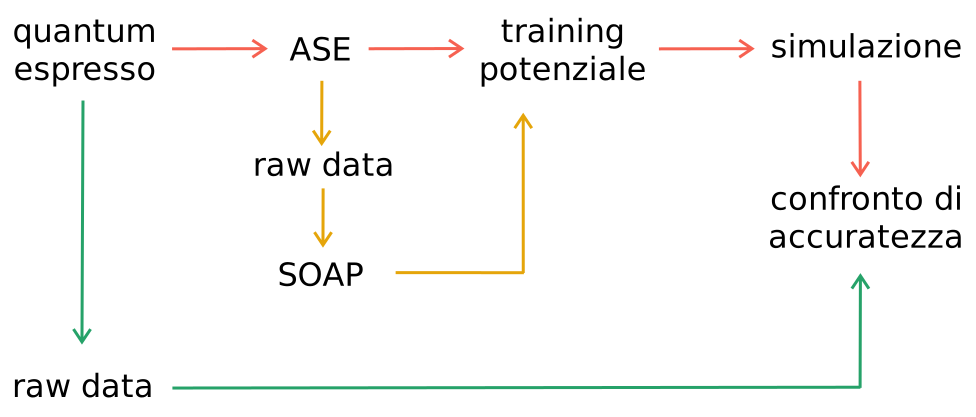
\includegraphics[scale=0.40]{./img/schema-lavoro.png}
    \captionof{schema}{Struttura schematica del processo di creazione dei feature vector}
    \label{sch:processo-creazione-feature-vector}
\end{figure}



\section{Quantum Espresso}

Quantum Espresso \cite{qe-2009, qe-2017, qe-2020} è il motore della dinamica molecolare, esso si occupa di utilizzare i principi della meccanica quantistica per produrre i frame che descrivono la dinamica molecolare per il materiale in esame.


    


\section{SOAP}
In questa sezione ci poniamo come obiettivo quello di dare una breve ma adeguata spiegazione, per quanto possibile completa e chiusa, del metodo SOAP (Smooth Overlap of Atomic Positions). 

Il punto fondamentale per comprendere la necessità di utilizzare una procedura come SOAP risiede nel concetto di invarianze fisiche. È infatti comune per le leggi della fisica essere invarianti per determinate proprietà, come lo possono essere le rotazioni, le traslazioni spaziali e lo scambio tra atomi uguali. Queste simmetrie emergono in modo naturale dalle leggi utilizzate, ma come un fisico deve impararle e con fatica ricavarle, anche un modello di ML necessiterebbe di imparare queste simmetrie ogni singola volta e questo richiede una spesa sia dal punto di vista computazionale che da quello temporale. Questo problema viene facilmente risolto utilizzando una rappresentazione che sia naturale espressione delle simmetrie del sistema, in questo modo non sarà necessario il training sulle simmetrie, rendendo il tutto più semplice.

\subsubsection{Generazione della mappa di densità}

Il primo step è quello di costruire la densità atomica associata a un determinato $Z$ tramite una funzione gaussiana. Questo ci permette di passare da una forma discreta a una continua, ottenibile applicando la seguente formula:

%\begin{equation}
%    \LARGE
%    \fcharDensity_Z (\,\uaVecr{r}\,) = \sum_{\alpha}^{Z} e^{-\frac{|\,\uaVecr{r}-\uaVecr{r}_{\alpha}\,|^2}{2\sigma^2}}
%\end{equation}

\begin{equation}
    \rho_Z (\vec{r} \,) = \sum_{\alpha}^{Z} e^{-\frac{|\vec{r}-\vec{r}_{\alpha}\,|^2}{2\sigma^2}}
    \label{eq:density-map-formula}
\end{equation}

quello che stiamo facendo è considerare un atomo con $Z$ fissato qualunque come l'origine di un sistema di coordinate e per ogni singolo atomo $\alpha$ con lo stesso numero $Z$ costruiamo una gaussiana. Nella formulazione \eqref{eq:density-map-formula} $r_{\alpha}$ indica la distanza tra il centro dell'atomo $\alpha$ vicino e quello centrato con il sistema di riferimento definito sopra. Questa struttura possiede quindi un picco in presenza dell'atomo. Dato che $\sigma$ viene utilizzato per definire lo zoom con cui analizziamo il sistema, minore è il valore di $\sigma$ più il risultato sarà perturbato anche da minime modifiche alla struttura, come una piccola modifica alla lunghezza dei legami (e conseguentemente della posizione relativa).

Questo step viene ripetuto per ogni singolo atomo, ottenendo come risultato che ogni atomo ha una mappa di densità dei suoi vicini, associata a esso.

Il fine ultimo della procedura descritta è quello di slegarci dal sistema di coordinate, usando infatti solo informazioni riguardanti la posizione relativa, rendiamo il tutto invariante per traslazioni. La somma su tutti gli atomi con il medesimo $Z$ rende inoltre invariante la rappresentazione rispetto allo scambio di due atomi uguali. La nuvola che viene così creata non è invariante per rotazioni, in quanto, se il centro del sistema di riferimento temporaneo menzionato sopra non è simmetrico per rotazione, allora non lo sarà neanche la nuvola risultante.

Nel caso siano presenti elementi con diverso numero atomico, come non di rado succede, la mappa di densità viene separata in base a esso, quindi, nel caso avessimo $Z_1$ e $Z_2$ allora avremo due mappe distinte, $\rho_{Z_1}$ e $\rho_{Z_2}$. Questo mantiene l'invarianza per permutazione e permette anche di distinguere le diverse specie chimiche presenti.


Vogliamo dare adesso una rappresentazione grafica di questo concetto, facciamo riferimento alla seguente immagine (\ref{fig:soap-step1-example}):

\begin{figure}[h]
    \centering
    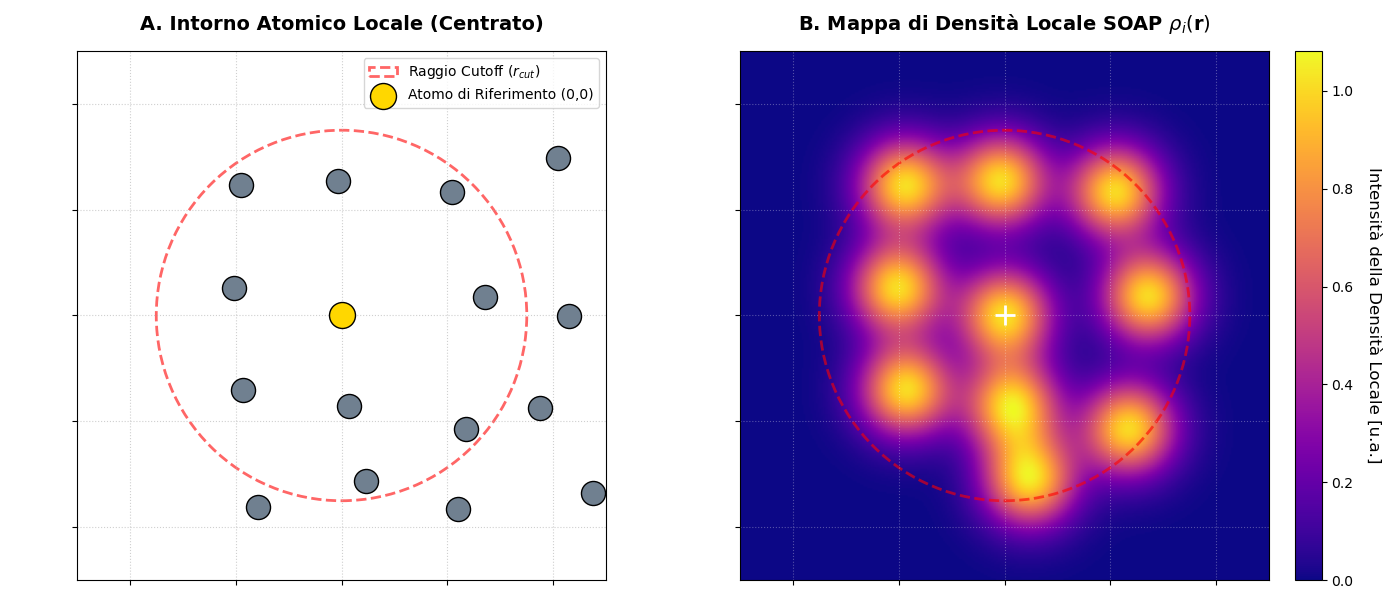
\includegraphics[scale=0.35]{./img/soap-step1-example.png}
    \caption{Rappresentazione generata tramite matplotlib del primo step della procedura SOAP}
    \label{fig:soap-step1-example}
\end{figure}

questa immagine è la somma di tutte le singole mappe prodotte per gli atomi interni al $r_{cut}$, dove è stato preso come riferimento l'atomo color oro posto al centro del sistema di coordinate. Il risultato finale si ottiene prendendo come atomo color oro, a turno, ognuno degli atomi presenti. Per semplicità di rappresentazione la struttura atomica è stata generata aggiungendo rumore a un cristallo periodico, questo non rappresenta nessuna struttura particolare, è solo una semplice griglia sulle cui intersezioni è stato posizionato un generico atomo.

Il controllo che viene dato dal parametro $\sigma$ della gaussiana è rappresentato nella seguente immagine (\ref{fig:soap-step1-example-sigma-big_small}):

\begin{figure}[h]
    \centering
    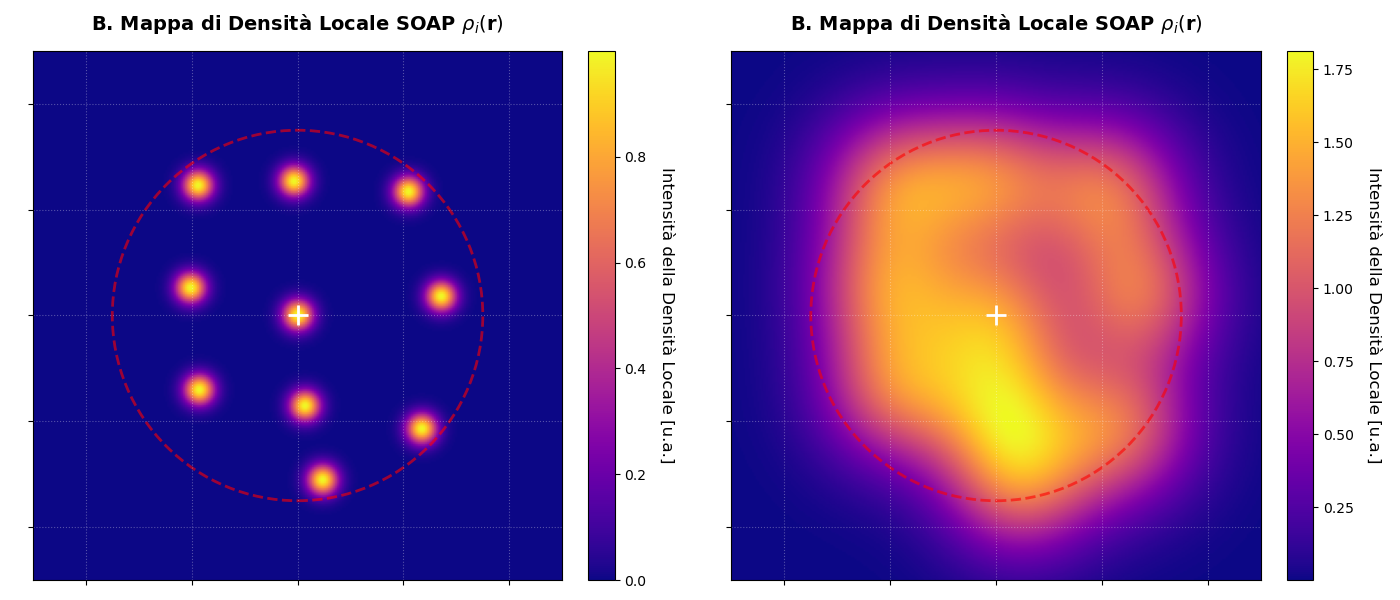
\includegraphics[scale=0.35]{./img/soap-step1-example-sigma-big_small.png}
    \caption{Rappresentazione generata tramite matplotlib del primo step della procedura SOAP per diversi valori del parametro $\sigma$}
    \label{fig:soap-step1-example-sigma-big_small}
\end{figure}

dove il pannello a sinistra rappresenta il caso di una $\sigma$ eccessivamente piccola e quello a destra il caso di una $\sigma$ eccessivamente grande. In entrambi i casi è possibile notare come l'informazione che se ne ricava non sia adeguata agli scopi descritti sopra. Infatti, come detto, vogliamo che l'aggiunta di una piccola quantità di rumore non modifichi in modo sensibile il fattore di somiglianza tra le due strutture. Nel primo caso la minima variazione di posizione porta a decretare che gli ambienti sono sensibilmente diversi, mentre nel secondo caso, anche una decisa modifica delle posizioni porta alla conclusione che i due ambienti siano simili.

Per quanto riguarda il valore di $r_{cut}$, esso controlla il significato che diamo ad "atomi vicini". Se fosse troppo piccolo si perdono informazioni riguardanti la struttura in esame, mentre se troppo grande arriviamo ad avere un vettore di feature complesso e pesante che non fornisce particolari vantaggi.

\subsubsection{Espansione in funzioni di base}
A questo punto ci poniamo di trovare un metodo che ci permetta di riassumere in modo compatto una funzione continua come quella rappresentata dalla mappa di densità. Per fare questo ci procuriamo delle funzioni di base, nel nostro caso radiali e angolari.

L'espansione in serie per la mappa di densità è data dalla formula:

\begin{equation}
    \rho_Z(\vec{r}) = \sum_{n=1}^{n_{max}} \sum_{l=0}^{l_{max}} \sum_{m=-l}^{l} c_Z(n,l,m) g(r \,;n) Y(\theta, \phi \,; l,m)
\end{equation}

dove il ; è posto a separatore tra le variabili e i parametri da cui dipendono le funzioni. Il coefficiente $c_Z$ è per la relativa specie in considerazione, come indicato sopra in presenza di specie diverse si costruiscono mappe separate.

In particolare si ha che:

\begin{equation}
    c_Z(n,l,m) = \int_{\mathbb{R}^3} \mathrm{d}r\, \mathrm{d}\theta\, \mathrm{d}\phi \;\; g(r \,;n) Y(\theta, \phi \,; l,m) \rho_Z(\vec{r}) 
\end{equation}

dove le $g(r \,;n)$ sono funzioni radiali e $Y(\theta, \phi \,; l,m)$ sono armoniche sferiche. Quello che stiamo andando a determinare tramite il coefficiente $c_Z$ è la "misura" della nostra mappa di densità lungo una determinata componente di base, in questo caso, funzioni radiali e armoniche sferiche (si utilizzano queste funzioni per le loro proprietà matematiche). Possiamo quindi adesso utilizzare questi coefficienti (un semplice vettore numerico) per ricostruire un oggetto tridimensionale come lo è la mappa di densità. 

In questa sezione non ci dilunghiamo sui dettagli della forma di queste funzioni.

Lo scopo di questo step è quello di semplificare la rappresentazione, come detto passiamo da una struttura tridimensionale complessa a un singolo vettore numerico. Non abbiamo ancora aggiustato le restanti invarianze in quanto, alla fine di questo step manca ancora l'invarianza per rotazione, la sua risoluzione sarà il cardine dello step successivo.

\subsubsection{Calcolo del power spectrum}

Per rendere la nostra rappresentazione invariante per rotazioni andiamo a calcolare il power spectrum parziale, ottenuto dalla seguente equazione:

\begin{equation}
    p_{Z_1Z_2}(n,n',l) = \pi \sqrt{\frac{8}{2l+1}} \sum_{m=-l}^{l} \overline{c_{Z_1}}(n,l,m) c_{Z_2}(n',l,m)
    \label{eq:power-spectrum}
\end{equation}

dove il primo coefficiente è sotto complessa coniugazione, nel caso si usino solo armoniche sferiche reali, essa diventa superflua. La presenza di $Z_1$ e $Z_2$ indica che questo viene calcolato per ogni coppia unica (indipendentemente dall'ordine) di specie chimiche presenti. Nel contesto del dataset A, quello che si produce è $(Z_{Ta},Z_{Ta})$, $(Z_{O},Z_{O})$ e $(Z_{Ta},Z_{O})$.

Senza entrare nei dettagli, diciamo che questo processo rende il risultato invariante dal punto di vista delle rotazioni, in quanto, le rotazioni possono essere rappresentate tramite matrici unitarie (oppure ortogonali nel caso reale). Il processo descritto sopra "trasforma" la matrice di rotazione (con cui possiamo rappresentare la rotazione della mappa di densità rispetto a un qualunque sistema di riferimento) nella matrice identità, che quindi non modifica il valore del coefficiente.

Le correlazioni che si trovano per valori di $Z_1$ e $Z_2$ diversi tra loro servono per tenere traccia delle posizioni relative delle diverse specie atomiche.

\subsubsection{Risultato finale}

Dopo aver calcolato tutti i vari elementi del power spectrum, si strutturano come un vettore, la cui dimensione viene determinata dalla seguente formula:

\begin{equation}
    \mathrm{dimensione} = (l_{max} + 1) \,\frac{1}{2}\, (S\cdot n_{max}) (S\cdot n_{max} +1)
    \label{eq:formula-dimensione-semplificata}
\end{equation}

Dove $S$ rappresenta il numero totale di specie diverse presenti nel materiale in analisi, $n_{max}$ e $l_{max}$ sono gli stessi parametri precedentemente definiti. 

Per una spiegazione su come ottenere questa formula si veda \autoref{app:dimpowspec}.


\subsubsection{Schema riassuntivo}

Diamo adesso una rappresentazione riassuntiva del processo completo (\autoref{fig:schema-riassunto-soap}), compresa anche la possibilità di dinamica molecolare suddivisa per frame. In particolare, il metodo di archiviazione della struttura di SOAP e la sua indicizzazione / organizzazione è lasciato pienamente in gestione alle librerie utilizzate, notiamo che l'ordine del vettore di feature non è trascurabile.

\begin{figure}[h]
    \centering
    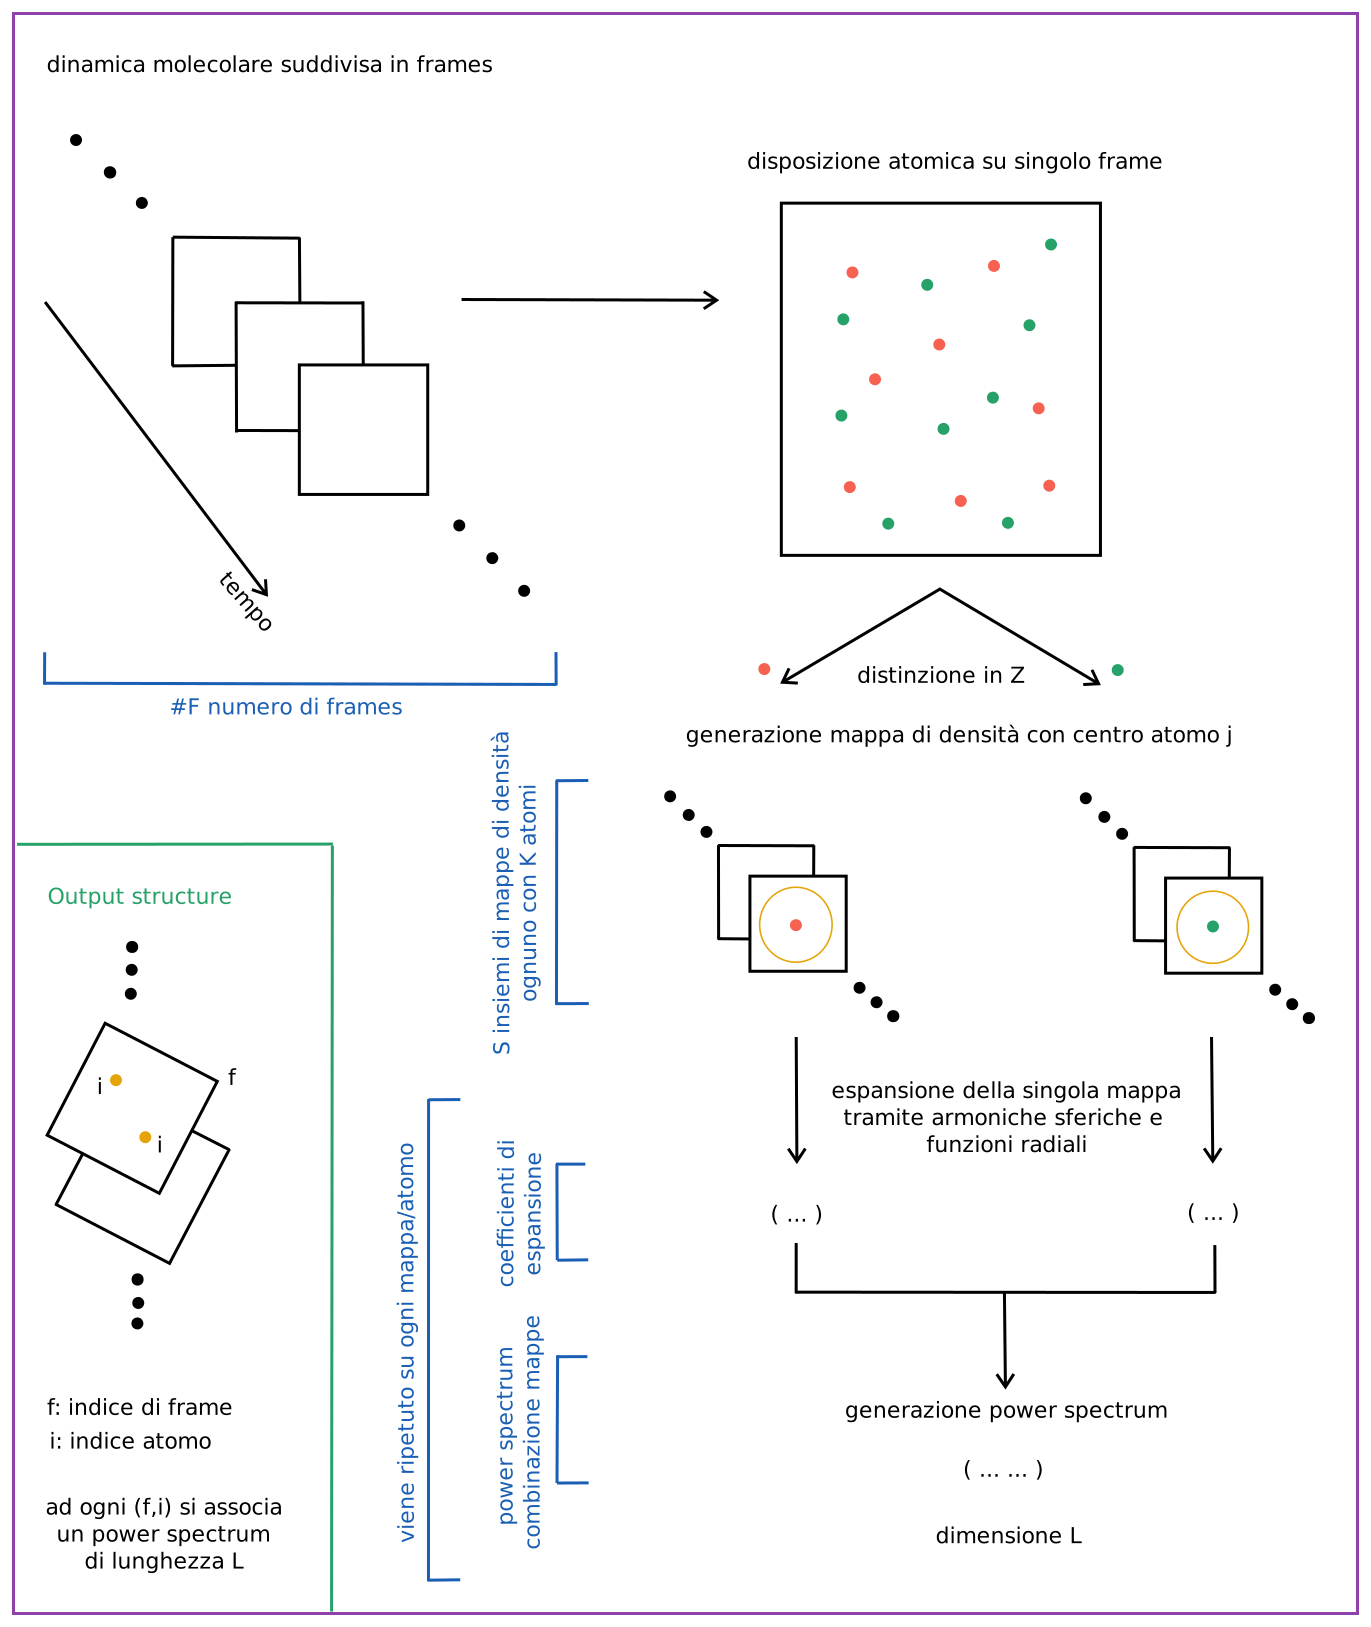
\includegraphics[scale=0.35]{./img/schema-riassunto-soap.png}
    \caption{Rappresentazione schematica della totalità del processo SOAP}
    \label{fig:schema-riassunto-soap}
\end{figure}

\clearpage

\section{Potenziali GAP}

Lo step successivo alla descrizione di un ambiente atomico tramite SOAP è quello di generare un potenziale che sia poi utilizzabile per fare previsioni di dinamica molecolare.
Il metodo che abbiamo deciso di utilizzare in questa analisi è quello dei potenziali GAP (Gaussian Approximation Potentials), questa tecnica si basa sul concetto della GPR (Gaussian Process Regression).

Il core concept di questo metodo è quello di scomporre l'energia totale del sistema nella somma dei singoli contributi atomici. Come per SOAP vogliamo utilizzare una descrizione locale per poter ottenere una complete picture del sistema in esame.

\begin{figure}[h!]
    \centering
    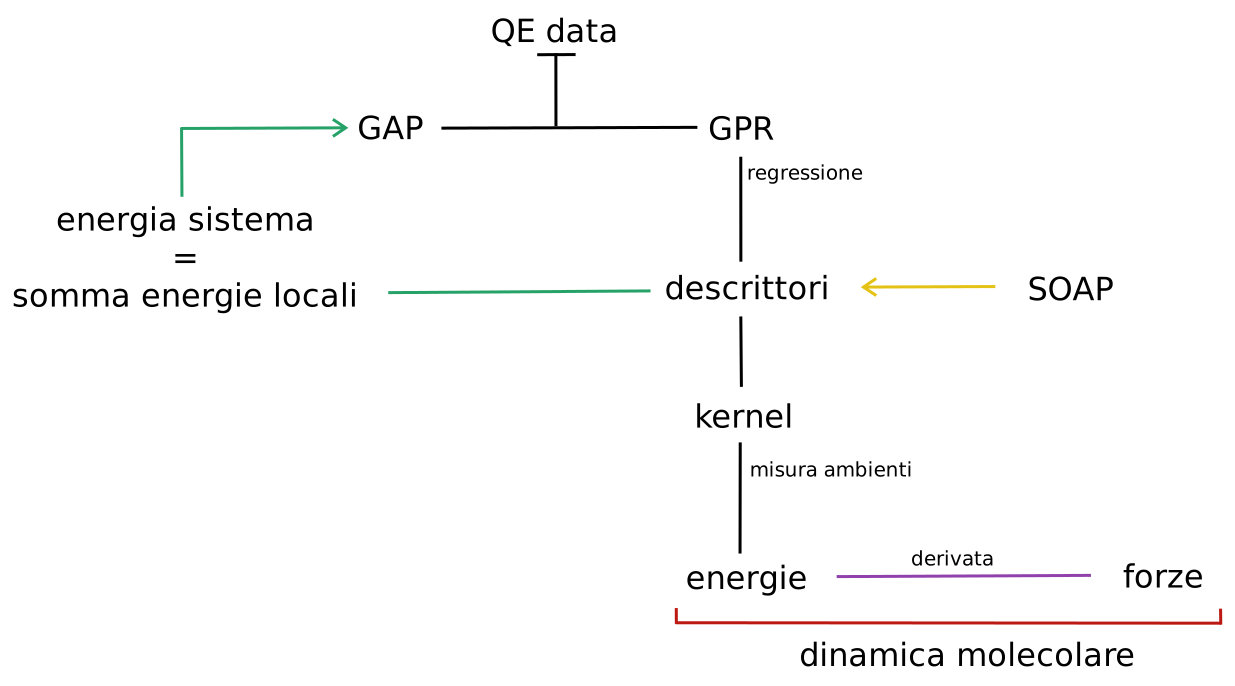
\includegraphics[scale=0.35]{./img/gap-schema.png}
    \captionof{schema}{Struttura schematica del framework GAP}
    \label{sch:schema-gap}
\end{figure}

Lo schema (\ref{sch:schema-gap}) descrive l'insieme di elementi che costituiscono il framework di un potenziale GAP.

Il processo matematico su cui si basa un potenziale GAP è la GPR (Gaussian Process Regression). 
Essendo questo un argomento vasto, anche per le innumerevoli applicazioni, nel seguito diamo una breve spiegazione del suo funzionamento senza soffermarci su particolari dettagli.

Il GPR è un metodo di regressione non parametrico, questo significa che non assumiamo che la relazione tra i dati abbia una specifica forma funzionale.
Questo ci permette di modellizzare sia relazioni non note che relazioni complesse.

Il processo ci permette di utilizzare la coppia di dati $(x, f(x))$ per generare una previsione del valore di $f$ in un punto che non appartiene al set di dati.

Per fare questa previsione utilizziamo un kernel (indicato spesso con $K$), ovvero una funzione che ci permette di definire la somiglianza tra due punti di input, esempio $(x_1, x_2)$, questo ci permette di imporre che punti tra loro vicini diano risultati non dissimili.
Inoltre possiamo utilizzare i parametri del kernel per definire le interazioni tra i punti, infatti in base alla distribuzione dei dati potrebbe essere necessario far parlare tra loro punti lontani, come nel caso di periodicità, oppure limitare l'interazione solo ai prossimi vicini.


Volendo dare alcuni dettagli aggiuntivi, quello che andiamo a fare è considerare l'insieme di tutte le funzioni $f$ che passando per l'insieme di punti $D$, il quale rappresenta i dati osservati.
Si costruisce una distribuzione di probabilità associata a queste funzioni, questa è una distribuzione gaussiana multivariata.
La funzione che cerchiamo è il valore di aspettazione di questa distribuzione e il kernel svolge il ruolo di matrice di covarianza.

Usiamo una spiegazione geometrica, nel caso più semplice possibile, per descrivere l'idea del processo, assumiamo di avere i dati $(x, f(x))$, possiamo assumere che $x$ segua una distribuzione gaussiana la cui media sia proprio il valore $f(x)$.

Possiamo vedere una rappresentazione della distribuzione gaussiana nella seguente immagine (\ref{fig:curva-gaussiana}).


Supponiamo adesso di voler prevedere il valore in un punto diverso che chiamiamo $x^*$. 
Consideriamo anche di aver precedentemente definito una funzione di kernel $K$, ricordiamo che questa dipende solo dai valori in input e non dai valori assunti dalla funzione.
Inoltre il valor medio di $f(x^*) = f^*$, lo conosciamo in quanto si assume un valore a priori, non entrando nei particolari, diciamo soltanto che si può assumere un valore sensato.
Abbiamo così costruito una distribuzione gaussiana bivariata.
Ricordando che sappiamo il valore di $f(x)$ possiamo "tagliare" la funzione bivariata in corrispondenza del noto $x$ e ottenere la distribuzione di $f^*$ dopo aver considerato i dati, da questa nuova distribuzione estraiamo il valor medio, esso è la nostra previsione.

La rappresentazione di questo concetto è data dall'immagine (\ref{fig:bi-gaussiana_e}), dove è evidenziato il taglio rispetto a uno specifico valore di $x$


{
	\begin{figure}[ht]
		\centering
		\begin{subfigure}{0.45\textwidth}
    		\centering
			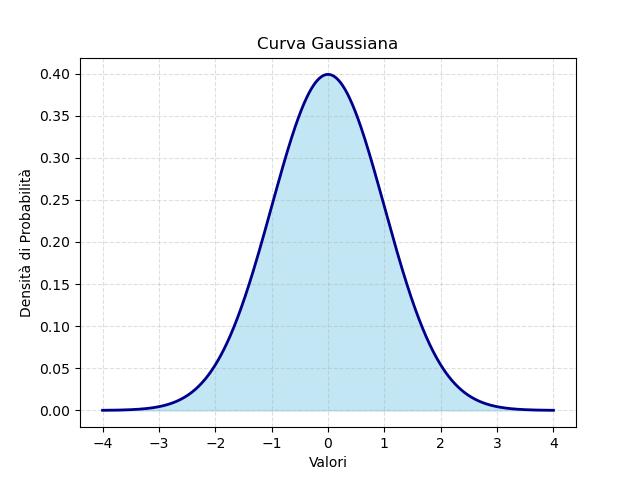
\includegraphics[scale=0.45]{./img/curva-gaussiana.png}
			\caption{Rappresentazione di una curva gaussiana}
			\label{fig:curva-gaussiana}
		\end{subfigure}
		\hfill
		\begin{subfigure}{0.45\textwidth}
    		\centering
			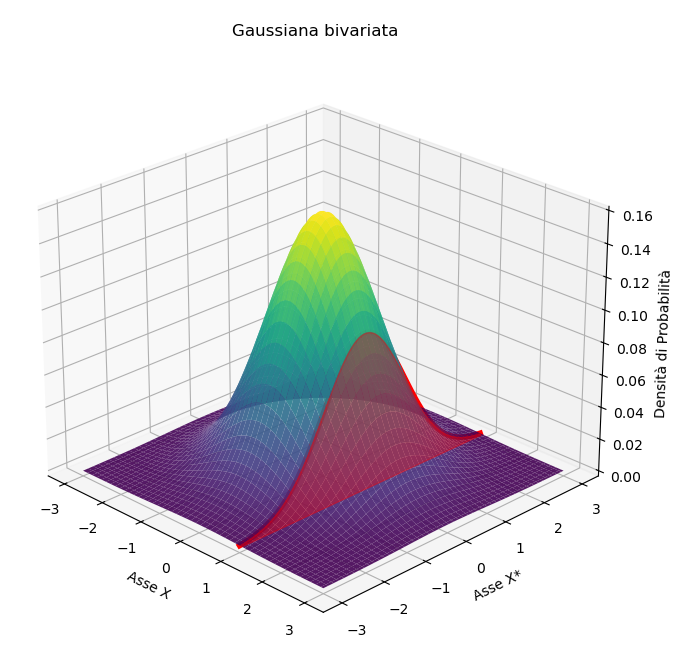
\includegraphics[scale=0.42]{./img/bi-gaussiana_e.png}
			\caption{Rappresentazione di una curva gaussiana bivariata}
			\label{fig:bi-gaussiana_e}
		\end{subfigure}
		\label{fig:gaussiane-sec-gap}
		\caption{}
	\end{figure}
}

Si generalizza, anche se con un pizzico di difficoltà, questo processo a un numero arbitrario di valori di input.

Vogliamo notare come qui non abbiamo trattato la stima delle incertezze sulle previsioni e di come incorporare l'incertezza di misura (come noise) sui dati osservati.


\section{Addestramento}

Per la fase di training usiamo dati generati da Quantum Espresso e un potenziale GAP. Partiamo esponendo in breve la struttura del processo che andremo a utilizzare.

La funzione svolta dal potenziale GAP è quella di associare determinate energie e forze, fornite come detto da QE, a una specifica configurazione geometrica, questa descritta tramite SOAP. 

Questa associazione viene poi utilizzata per indovinare il valore di energia di un atomo dato il suo intorno geometrico, in particolare, preso un atomo X ne viene calcolato il SOAP, questo, tramite una funzione di kernel, viene confrontato con gli ambienti della fase di training ed infine viene estratto un valore probabile per l'energia.
Data la struttura del metodo, un punto che vogliamo sottolineare è che l'accuratezza decresce velocemente fuori da scenari compatibili con i dati di training, è ovviamente possibile arginare se non risolvere il problema addizionando diverse tecnologie al metodo, queste non sono però esaminate in questa trattazione.

\section{Simulazione}

La parte di simulazione è stata divisa in tre diverse tipologie, ognuna di queste tentava di risolvere i problemi sorti durante la fase di analisi.

Di seguito vengono descritte, senza entrare troppo nei dettagli, le diverse procedure adottate.

\subsection{Simulazione NVE}

Per prima cosa abbiamo provato a svolgere una semplice simulazione di tipo NVE, questa prende il nome dalle quantità che si pone di conservare, ovvero il numero di particelle, il volume e l'energia totale.

Per questa si è usato come potenziale il GAP addestrato e per realizzarla la libreria ASE (si veda \autoref{subsec:simulazione-nve-ase}).

\subsection{Simulazione NVE con ZBL}

Questa simulazione prevede di utilizzare la stessa struttura vista alla sezione precedente, a cui viene addizionato un potenziale ZBL. Questo può essere inserito sia in fase di training del potenziale che come correzione successiva e in questo caso abbiamo deciso di adottare la seconda opzione. 

Lo ZBL (Ziegler-Biersack-Littmark) è un potenziale repulsivo che utilizza una repulsione coulombiana schermata, più precisamente esso ha la seguente formula:

\begin{equation}
    V(r_{ij}) = \frac{1}{4\pi\epsilon_0}\frac{Z_iZ_j}{r_{ij}} \phi\left(\frac{r_{ij}}{a_{ij}}\right)
\end{equation}

dove si riconosce nella prima parte, il potenziale di Coulomb, la funzione $\phi$ è detta \textit{funzione di schermatura universale}, questa permette di tenere in considerazione la schermatura prodotta dalla nuvola elettronica. La forma di questa funzione è stata ricavata tramite un fit su un grande numero di coppie di atomi e assume la forma seguente, data dalla somma di quattro esponenziali:

\begin{equation}
    \phi\left(\frac{r_{ij}}{a_{ij}}\right) = \phi(x) = 0.1818e^{-3.2x} + 0.5099e^{-0.9423x} + 0.2802e^{-0.4029x} + 0.02817e^{-0.2016x}
\end{equation}

dove con $a_{ij}$, detto \textit{lunghezza di schermatura universale}, la schermatura viene adattata alla dimensione degli atomi coinvolti. In particolare:

\begin{equation}
    a_{ij} = \frac{0.8854\, a_0}{Z_i^{0.23} + Z_j^{0.23}}
\end{equation}

dove $a_0$ è il raggio di Bohr.

L'implementazione nel nostro caso ha un termine aggiuntivo, una funzione di smoothing: 

\begin{equation}
    S(u) = -6u^5 + 15u^4 - 10u^3 +1
\end{equation}

\begin{equation}
    u = \frac{r-r_{inner}}{r_{outer}-r_{inner}}
\end{equation}

questo permette di eliminare le discontinuità quando vengono calcolate le forze, infatti agli estremi la derivata di questa funzione si annulla.

I parametri $r_{inner}$ e $r_{outer}$ rappresentano rispettivamente la distanza a cui il potenziale assume il valore massimo, ovvero la funzione di smoothing assume valore 1, e la distanza a cui il potenziale repulsivo si annulla. Possiamo immaginare che questi valori rappresentino delle sfere di influenza.

\subsection{Simulazione Monte Carlo con algoritmo di Metropolis}
\label{subsec:simulazione-metropolis-teoria}

Questo tipo di simulazione prevede un cambio di paradigma rispetto a quello che abbiamo visto precedentemente.
Per prima cosa partiamo considerando il nostro sistema composto da $126$ atomi, tra \ce{Ta} e \ce{O}, a questo possiamo associare uno \textit{spazio delle configurazioni} ($3N$), ovvero uno spazio nel quale ogni punto rappresenta in modo univoco una configurazione del nostro sistema. 

Questa simulazione abbandona la dinamica molecolare e ci fa invece esplorare questo spazio, che contiene anche tutte le possibili configurazioni ottenute tramite dinamica molecolare una volta fissate le condizioni al contorno.

Ogni configurazione spaziale ha un'energia potenziale associata, utilizzando questa energia e la temperatura di riferimento a cui vogliamo studiare il sistema, possiamo calcolare la probabilità che il sistema si trovi in questa particolare configurazione, questo si ottiene tramite la \textit{distribuzione di Boltzmann}:

\begin{equation}
    P(A) \propto \mathrm{exp}\left(-\frac{E_{pot}(A)}{k_b\,T}\right)
\end{equation}

nel seguito ci riferiremo all'energia potenziale solo con il termine di energia e con il simbolo $E$, in quanto questa è l'unica che consideriamo.

Dati questi elementi, vogliamo determinare un metodo che ci permetta di decidere quali stati sono accettabili per il sistema e, per prima cosa, determiniamo la differenza di energia tra due stati "consecutivi"

\begin{equation}
    \Delta E = E_{new} - E_{old}
\end{equation}

dove con stati "consecutivi" intendiamo due stati, la cui differenza nello spazio delle configurazioni è data da una perturbazione che abbiamo introdotto noi.

Possiamo distinguere tra due scenari:

\begin{itemize}
    \item $\Delta E \leq 0$ lo stato \texttt{new} ha energia minore del precedente
    \item $\Delta E > 0$ lo stato \texttt{new} ha energia maggiore del precedente
\end{itemize}

da cui calcoliamo la probabilità di accettare la transizione a questo nuovo stato come:

\begin{equation}
    P_{acc} = \mathrm{exp}\left(-\frac{\Delta E}{k_bT} \right)
\end{equation}

In ultimo, per determinare se lo stato viene accettato oppure rifiutato, generiamo un numero casuale compreso tra zero e uno e nel caso in cui il numero sia minore di $P_{acc}$ allora lo stato viene accettato e la configurazione \texttt{new} diventa il nuovo punto di partenza, altrimenti manteniamo la configurazione \texttt{old}.

Rappresentiamo questo processo con lo schema (\ref{sch:markov-chain-schema}) dove, senza dare ulteriori dettagli, è possibile riconoscere la struttura di una Markov chain.

\begin{figure}[h!]
    \centering
    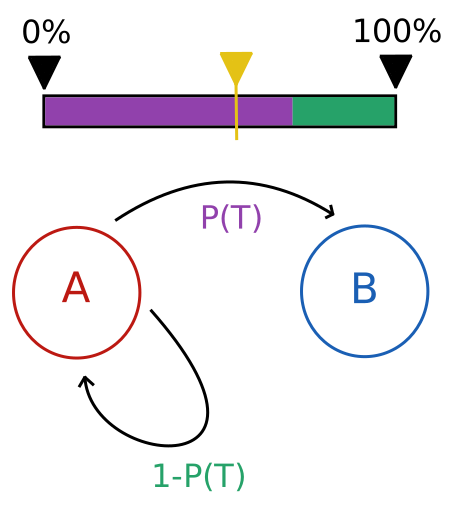
\includegraphics[scale=0.37]{./img/markov-chain-schema.png}
    \captionof{schema}{Struttura schematica dell'algoritmo di Metropolis}
    \label{sch:markov-chain-schema}
\end{figure}

Con $P(T)$ intendiamo la probabilità di accettazione, che in questo contesto abbiamo definito come probabilità di transizione, lo slider giallo rappresenta invece il valore in cui è caduto il numero casuale estratto, così nello schema visualizzato la transizione è accettata e si passa dalla configurazione A alla configurazione B. Questo stesso identico schema si ripete per ogni singolo stato proposto.

    \chapter[Python]{Discussione sulle librerie e sul codice python utilizzato}


\section{ASE} %----------------------------------------------------------------------------------------------------------------------------------------------------------------------------------------------------
La libreria \cite{ase-doc} ci permette di analizzare le simulazioni di dinamica molecolare prodotte tramite QE. Essenzialmente possiamo dire che essa svolge il ruolo di ponte tra una struttura fatta di coordinate e una che sia computazionalmente utilizzabile. Questo ci permette di trasportare le informazioni che QE utilizza per svolgere i calcoli, come le condizioni di periodicità, in un formato poi accessibile anche da altre librerie.
Inoltre questa libreria rende possibile svolgere semplici simulazioni di dinamica molecolare.
\\

\subsection{Lettura dei file di Quantum Espresso}

In particolare per QE abbiamo utilizzato i seguenti:

\begin{lstlisting}[caption={Snippet usato per il dataset A}, label={code:ase-dataset-a}, language=Python]
    frame = ase.io.read(file_name, index=":", format="espresso-out")
\end{lstlisting}

dove \texttt{index=":"} viene utilizzato per leggere tutti i frame presenti nel file di input e \texttt{format="espresso-out"} serve per impostare la tipologia di file da leggere.
\footnote{
La specifica sezione della documentazione è reperibile al seguente link: \url{https://ase-lib.org/ase/io/io.html}
}

La funzione \texttt{read} ci restituisce un oggetto di tipo \texttt{atoms}
\footnote{
La specifica sezione della documentazione è reperibile al seguente link: \url{https://ase-lib.org/ase/atoms.html}
}, che costituisce l'oggetto python che contiene le informazioni che definiscono il materiale da simulare, estratte dai file di output di QE.


\subsection{Simulazione con un potenziale ML}

I potenziali generati tramite ML vengono utilizzati come dei \textit{calculator} \footnote{Si veda la documentazione: \url{https://docs.ase-lib.org/ase/calculators/calculators.html}} per la dinamica molecolare.
Questo oggetto può essere descritto come una calcolatrice che data una configurazione restituisce i valori delle energie e delle forze.

Lo step successivo è utilizzare un motore di dinamica molecolare \footnote{Si veda la documentazione: \url{https://docs.ase-lib.org/ase/md.html}}
per muovere gli atomi e ottenere il frame successivo.

Diamo adesso una descrizione del codice utilizzato per svolgere questo processo, notiamo che il potenziale addestrato tramite QUIP (si veda \autoref{sec:quippy}), deve essere caricato tramite la libreria quippy, essendo necessario per la discussione sulla dinamica molecolare, lo riportiamo in questa sezione.

\begin{lstlisting}[caption={Loading del potenziale addestrato}, label={code:potential-loading-ase-md}, language=Python]
    from quippy.potential import Potential
    
    calc = Potential(param_filename=file_potenziale)
    calc.name_ = "GAP" 
\end{lstlisting}

Sarà poi possibile associare il calcolatore \texttt{calc} a un oggetto \texttt{atoms} di ASE tramite \verb|atomi.calc = calc|.

\subsubsection{Simulazione NVE}
\label{subsec:simulazione-nve-ase}

La simulazione NVE impone la conservazione dell'energia totale del sistema, oltre al volume e al numero di particelle.

Abbiamo impostato la simulazione al modo seguente, la versione riportata è una semplificazione del codice effettivamente utilizzato:

\begin{lstlisting}[caption={Simulazione NVE}, label={code:simulation-nve-ase-md}, language=Python]
    from ase.io import read
    from ase.md.verlet import VelocityVerlet
    from ase.md.velocitydistribution import MaxwellBoltzmannDistribution
    from ase import units

    #Lettura della configurazione iniziale da file di QE
    atomi = read(PATH_CONFIG_INIZIALE, index=0)

    #Setting del calcolatore
    atomi.calc = calc

    #Setting delle velocità iniziali
    MaxwellBoltzmannDistribution(atomi, temperature_K=3000)

    #Setting della dinamica molecolare
    dyn = VelocityVerlet(
          atomi, 
          timestep=TIMESTEP, 
          trajectory=PATH_TRAJ_OUTPUT,
          logfile=PATH_LOG_OUTPUT,
          loginterval=1 )     
          
    #Avvio della simulazione
    dyn.run(passi_totali)
\end{lstlisting}

per le velocità iniziali, si è provato a reperirle dal file di QE, ma questo non le riportava, sono quindi state estratte dalla distribuzione di Maxwell-Boltzmann.


\section{DScribe} %------------------------------------------------------------------------------------------------------------------------------------------------------------------
DScribe è la libreria \cite{dscribe-doc} che si occupa di trasformare la struttura atomica, definita tramite ASE, in un qualcosa di comprensibile dai modelli di ML. Lo scopo principale di questa procedura è quello di rendere il training di un modello il più semplice possibile. L'idea è quella di creare un oggetto che identifichi in modo univoco una determinata struttura atomica e che sia invariante per modifiche "matematiche" della struttura stessa, come possono esserlo le rotazioni; se così non fosse, il modello dipenderebbe da un sistema di coordinate e andrebbe sottoposto a training anche per le diverse rotazioni. Questo processo porta alla produzione di un descriptor, o vettore di feature, che contiene l'informazione sulle invarianze delle leggi fisiche che descrivono il sistema. La prima cosa che facciamo notare è che separando il descriptor dalla fase di training è possibile riutilizzarlo con un diverso modello, diminuendo così il tempo necessario per l'addestramento. Abbiamo deciso di utilizzare il descriptor SOAP, per la rappresentazione locale della struttura atomica in analisi. \cite{dscribe-intro,dscribe2}
\\

Riportiamo adesso l'uso che abbiamo fatto di questo pacchetto:

\begin{lstlisting}[caption={Snippet usato per la creazione delle feature tramite SOAP}, label={code:soap-dscribe}, language=Python]
    soap_obj = SOAP(
        species= ,  # tutti gli atomi nella struttura in esame
        periodic= , # condizione di periodicità    
        r_cut= ,    # raggio di cutoff
        n_max= ,    # numero funzioni radiali     
        l_max=      # grado massimo armoniche sferiche )
    features = soap_obj.create(QE_data, n_jobs=-1)
\end{lstlisting}

dove \texttt{soap\_obj} è una configurazione per SOAP, \texttt{species} definisce tutti gli atomi che saranno incontrati nella struttura in esame, \texttt{periodic} serve per impostare l'uso della struttura periodica (precedentemente definita in ASE), \texttt{r\_cut} definisce un cutoff per la rappresentazione locale (espresso in \r{A}), \texttt{n\_max} è il numero di funzioni radiali di base, \texttt{l\_max} il massimo grado delle armoniche sferiche \footnote{La documentazione è reperibile al seguente: \url{https://singroup.github.io/dscribe/latest/tutorials/descriptors/soap.html}}. Il parametro $\sigma$ discusso in equazione \eqref{eq:density-map-formula} assume come valore predefinito 1.

In particolare, l'accuratezza della rappresentazione, come il numero delle feature, cresce proporzionalmente al valore di \texttt{n\_max} e \texttt{l\_max}.

La funzione \texttt{create} si occupa poi di creare il vero e proprio SOAP, in input viene passato \texttt{QE\_data}, ovvero la struttura atomica in analisi definita tramite la libreria ASE.

Il risultato di questi calcoli è un complesso oggetto, indicizzato come segue:

{\centering \verb|[num frame, num atomi, feature vector]|}

Vogliamo far notare che questa libreria è stata utilizzata solo inizialmente per verificare la possibilità di utilizzare SOAP sui dati a nostra disposizione, successivamente l'intero processo è stato svolto da QUIP.


\subsubsection{Note sulla struttura matematica} 

DScribe, in particolare, per le armoniche sferiche usa la loro versione puramente reale, in modo da evitare l'utilizzo dell'algebra complessa e come funzioni radiali delle GTO (Gaussian Type Orbitals) tali da rendere il tutto computazionalmente veloce e accurato.


\section{Quippy} %-----------------------------------------------------------------------------------------------------
\label{sec:quippy}

Quippy è la libreria che si occupa della gestione del potenziale GAP \cite{quip-doc, quip-gap-doc}.

In particolare andremo a utilizzare la funzione \texttt{gap\_fit} 
\footnote{La documentazione è reperibile al seguente: \url{https://libatoms.github.io/GAP/gap_fit.html} }


\begin{lstlisting}[caption={Snippet per il calcolo del GAP}, label={code:gap-libatom}, language=bash]

    gap_fit 
    at_file=               #nome file.extxyz con i dati di training 
    default_sigma={        #definisce le incertezze sui dati:
                   -       #incertezza sull'energia
                   -       #incertezza sulle forze 
                   -       #non presente nei dati
                   -       #non presente nei dati }
                    
    gap={soap                #tipologia di descrittore, nel 
                             # nostro caso SOAP
        l_max=               #numero funzioni radiali
        n_max=               #grado massimo armoniche sferiche  
        atom_sigma=          #"zoom" della mappa di densità  
        zeta=                #esponente per il kernel
        cutoff=              #raggio di cutoff
        covariance_type=     #tipologia di kernel per il 
                             # confronto degli ambienti
        n_sparse=            #numero punti per lo sparse method
        sparse_method=       #tipologia di sparse method
        delta=               # } 
    e0=                           #energia di atomo libero
    energy_parameter_name=energy  #config name per file input
    force_parameter_name=forces   #config name per file input
    gp_file=                      #nome file.xml di output 

\end{lstlisting}

dopo aver generato il file del potenziale, esso può essere utilizzato come \texttt{calculator} per la dinamica molecolare tramite ASE.


\section{Potenziale ZBL} %----------------------------------------------------------------------------------------------------------------------------------------------------

Il potenziale ZBL è stato implementato tramite una classe, in questo modo è possibile ereditare da ASE la struttura di un \texttt{calculator}. Di seguito diamo solo una breve parte del codice utilizzato.

\begin{lstlisting}[caption={Snippet per la classe che implementa il potenziale ZBL}, label={code:zbl-class-implementation}, language=python]

class class_zbl(Calculator):

    implemented_properties = ["energy", "free_energy", "forces"]

    def __init__(self, **kwargs): #----------
        super().__init__(**kwargs)

        self.coefficients = np.array([0.1818, 
                                      0.5099, 
                                      0.2802, 
                                      0.02817], dtype=float)
        self.exponents = np.array([3.2, 
                                   0.9423, 
                                   0.4029, 
                                   0.2016], dtype=float)

        self.raggio_inner = 0.0
        self.raggio_outer = 0.0

        self.checkandsetParameters()
    
    #setting dei parametri
    def checkandsetParameters(self): #------------

    #implementa la funzione di switch per il potenziale e la derivata della funzione di switch
    def switch(self, distances): #----------
        . . .
        return switch, dswitch_dr

    #implementa il vero e proprio calcolatore
    def calculate(self, atoms=None, properties=("energy",), system_changes=all_changes):
        super().calculate(atoms, properties, system_changes)
        . . .
        # Salvataggio nel dizionario interno di ASE
        self.results = {
            "energy": energy, 
            "free_energy": energy, 
            "forces": forces }
        
\end{lstlisting}

\section{Algoritmo di Metropolis}

Mostriamo in questa sezione una breve e schematica descrizione del codice utilizzato per implementare l'algoritmo di Metropolis come descritto in \autoref{subsec:simulazione-metropolis-teoria}.

\begin{lstlisting}[caption={Snippet per la classe che implementa l'algoritmo di Metropolis}, label={code:zbl-class-implementation}, language=python]

class class_makeMontecarlo:

    #facciamo un setting dei parametri generali che servono per ogni motore di simulazione
    def __init__(self): #----------

        #Data la struttura del codice di lettura dei parametri
        #il potenziale GAP deve essere caricato dentro questa funzione
        self.calc_gap = Potential(param_filename=setConfig.PATH_POTENZIALE)
        self.calc_gap.name_ = "GAP"

        #estrazione della configurazione di partenza
        self.atomi_md = read(setConfig.PATH_CONFIG_INIZIALE, index=0)
        #assegna il calcolare determinato sopra
        self.atomi_md.calc = self.calc_totale
        
        self.MCsteps = setConfig.PASSI_TOTALI * len(self.atomi_md) 
        #self.MCsteps: Numero totale di tentativi Monte Carlo
        
    #Esegue una simulazione Monte Carlo di Metropolis nell'insieme NVT.
    def runMetropolisMC(self):

        # Costante di Boltzmann in eV/K (da ase.units.kB)
        kbT = kB * setConfig.TEMPERATURE

        for step in range(1, self.MCsteps + 1):
            pos_proposte = pos_old.copy()

            if setConfig.MOVE_TYPE == 'single':
                # Scegliamo un singolo atomo casuale
                idx = np.random.randint(0, len(self.atomi_md))
                # Spostamento gaussiano o uniforme centrato in 0
                delta = np.random.uniform(-setConfig.MCSTEP_SIZE, 
                                          setConfig.MCSTEP_SIZE, 
                                          size=3)
                pos_proposte[idx] += delta

            # Applichiamo la configurazione proposta
            self.atomi_md.set_positions(pos_proposte)
            e_new = self.atomi_md.get_potential_energy()

            # Calcolo della differenza di energia
            delta_E = e_new - e_old

            # CRITERIO DI METROPOLIS ------------
            if delta_E <= 0:
                accettata = True
            else:
                p_acc = np.exp(-delta_E / kbT)
                accettata = (np.random.rand() < p_acc)

            # AGGIORNAMENTO DELLO STATO ---------
            if accettata:
                e_old = e_new
                pos_old = pos_proposte.copy()
                f_old = self.atomi_md.get_forces()
                stato = "ACCETTATA"
            else:
                # Ripristiniamo la geometria precedente
                self.atomi_md.set_positions(pos_old)
                stato = "RIFIUTATA"                
                dump = self.atomi_md.get_potential_energy()
                dump = self.atomi_md.get_forces()
                dump = None

\end{lstlisting}

il codice qui inserito non rappresenta fedelmente quello utilizzato in fase di simulazione, in quanto abbiamo presentato una versione semplificata al solo scopo di fornire un metodo di implementazione. In questo contesto abbiamo mostrato un codice che seleziona un atomo casualmente e muove solo esso per proporre una nuova configurazione. Con tale codice è anche possibile muovere simultaneamente tutti gli atomi del sistema.

Il ciclo \texttt{for} qui presentato è l'implementazione della Markov chain descritta nello schema \ref{sch:markov-chain-schema}.

    \chapter{Test: dataset A}


Il dataset A consiste dei risultati di una simulazione di MD eseguita con QE per una struttura amorfa costituita da \ce{Ta2O5}, pentossido di ditantalio (a cui ci riferiamo anche come tantala). 


Esso è composto da una serie di file di QE che costituiscono la dinamica molecolare di una struttura di tantala a circa $3'000$ K.

Usando la libreria ASE abbiamo generato una rappresentazione della cella atomica dai dati di QE analizzati, essendo questa una simulazione di dinamica molecolare, riportiamo solo uno degli step a cui diamo il nome di frame. L'immagine di seguito (\ref{fig:cristallo-from-ase-frame-0-dataset-a}) è stata generata tramite matplotlib.

\begin{figure}[h]
    \centering
    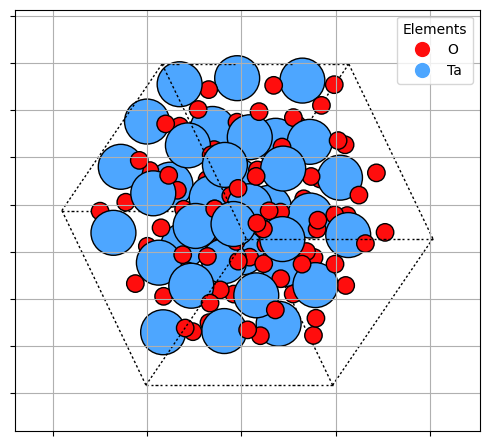
\includegraphics[scale=0.50]{./img/cristallo-from-ase-frame-0-dataset-a.png}
    \caption{Rappresentazione generata tramite ASE della struttura atomica del dataset A}
    \label{fig:cristallo-from-ase-frame-0-dataset-a}
\end{figure}


\section{SOAP con DScribe}

Considerando la discussione svolta per spiegare SOAP, unita alla spiegazione riguardante DScribe, vogliamo dare un esempio pratico di utilizzo del metodo considerando un contesto sul quale conosciamo già il risultato.

Dove abbiamo utilizzato il \autoref{code:soap-dscribe} nel seguente modo:

\begin{lstlisting}[caption={Snippet usato per il dataset A}, label={code:soap-dataset-a}, language=Python]
    soap_obj = SOAP(
        species=["Ta", "O"],
        periodic=True,       
        r_cut=5.0,      
        n_max=8,         
        l_max=6 )
    features = soap_obj.create(QE_data, n_jobs=-1)
\end{lstlisting}


\begin{tcolorbox}[
    center,
    fontupper=\footnotesize,
    colback=white,
    boxrule=0.8pt,
    colframe=gray!60,
    width=0.90\linewidth,
    arc=3mm
]
\textbf{Nota sui parametri}

Dato che ci stiamo ponendo come scopo quello di verificare che il metodo sia utilizzabile, i parametri riportati sopra non sono stati in alcun modo ottimizzati, essi sono stati reperiti negli esempi della documentazione. 
%Un test che si potrebbe svolgere per la loro ottimizzazione è un tradeoff tra velocità di calcolo e accuratezza dei risultati rispetto a quelli prodotti da Quantum Espresso.
\end{tcolorbox}


Consideriamo l'atomo 42 e calcoliamo un \textit{kernel} tra i frame successivi, questo significa che seguiamo un singolo atomo lungo tutta la dinamica molecolare.

Un kernel è una funzione che ci permette di misurare quanto due descrittori SOAP (il power spectrum) siano simili, e conseguentemente gli ambienti da cui derivano. Nel nostro caso usiamo il kernel più semplice possibile:

\begin{equation}
    \mathrm{Kernel}(\vec{p_1},\vec{p_2}) = \frac{\vec{p_1}\cdot\vec{p_2}}{|\vec{p_1}|\,|\vec{p_2}|}
    \label{eq:kernel-lineare}
\end{equation}

Il risultato che ci aspettiamo è che lungo tutti i frame il valore di questa funzione sia circa uno, data la struttura dei dati, infatti ogni frame rappresenta un piccolo scostamento temporale di una dinamica molecolare continua.

Se produciamo un grafico dove lungo l'asse x poniamo un indice (1 rappresenta il confronto tra il frame 1 e 2, e così per tutti gli altri indici) e sull'asse delle y mettiamo il valore del kernel otteniamo:

\begin{figure}[h]
    \centering
    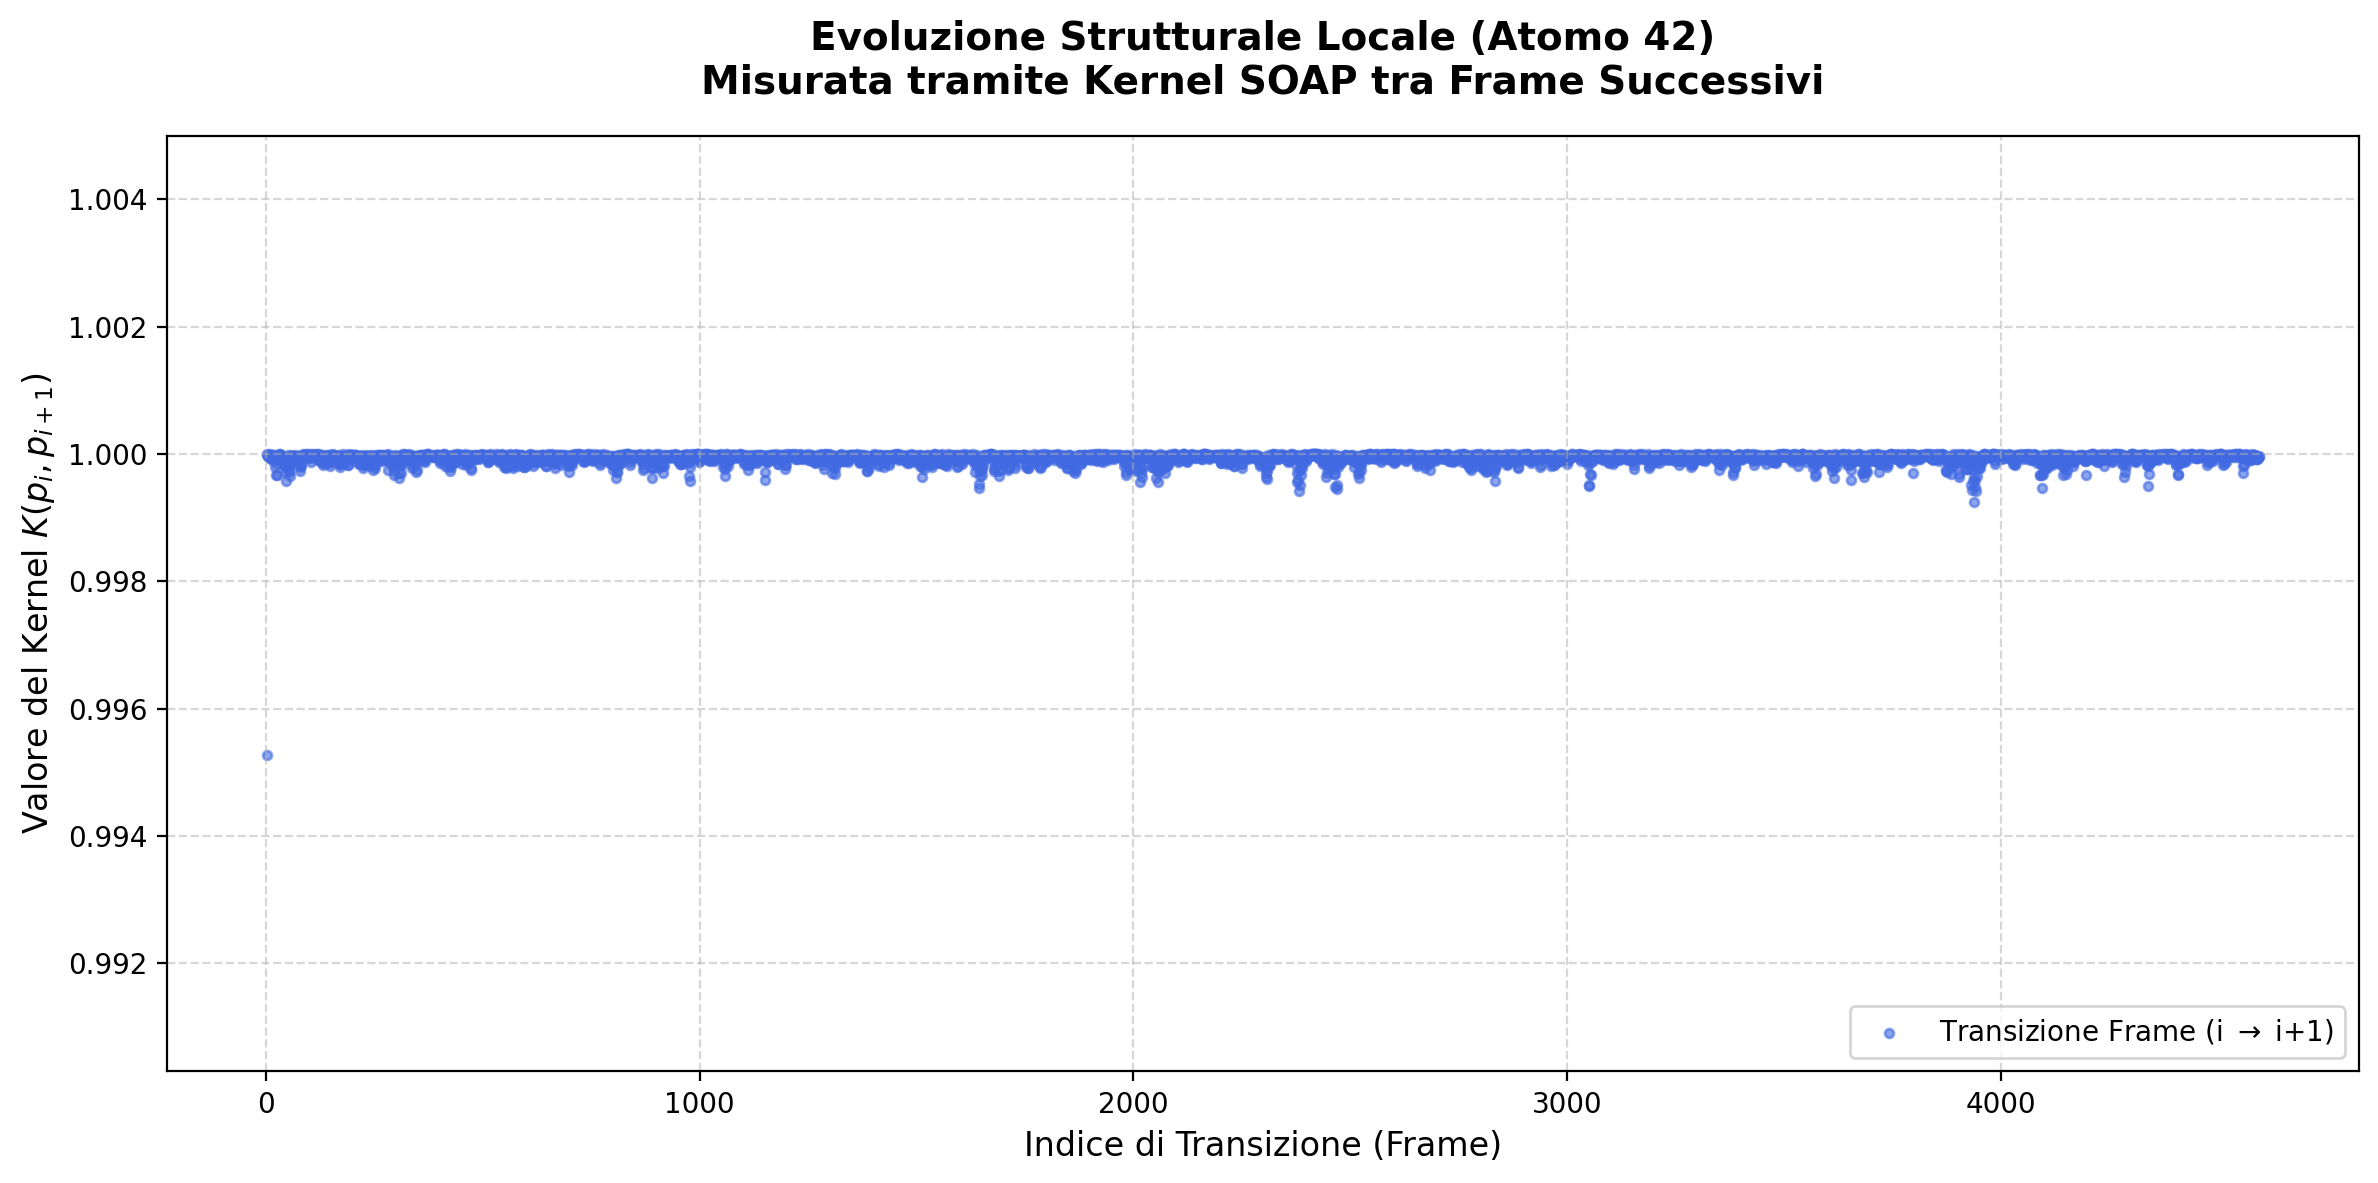
\includegraphics[scale=0.50]{./img/kernel.png}
    \caption{Rappresentazione del kernel per i frame del dataset A}
    \label{fig:kernel-dataset-a}
\end{figure}

Osservando la \autoref{fig:kernel-dataset-a}, il risultato è esattamente quello atteso, l'unico punto che si discosta è il primo ma non riteniamo questo punto particolarmente problematico.
\\

\clearpage

\section{Sessione di testing}
In questa sezione spiegheremo come è stato utilizzato il dataset A per sperimentare il funzionamento del workflow descritto nello schema \ref{sch:schema-gap}.

\subsection{Addestramento potenziale con Quippy}

\begin{lstlisting}[caption={Snippet usato per il calcolo del GAP per il dataset A}, label={code:gap-dataset-a}, language=bash]
    gap_fit 
    at_file=train_data.extxyz 
    default_sigma={0.0002 0.1 0.0 0.0} 
    gap={soap 
        l_max=2 
        n_max=2 
        atom_sigma=0.5 
        zeta=4 
        cutoff=5.0 
        covariance_type=dot_product 
        n_sparse=500 
        sparse_method=cur_points
        delta=1 } 
    e0={Ta:-9884.889316093:O:-561.82449957} 
    energy_parameter_name=energy 
    force_parameter_name=forces 
    gp_file=out_potenziale_gap-500-n2-l2.xml
    > potenziale_quippy-500-n2-l2.log

\end{lstlisting}

\begin{tcolorbox}[
    center,
    fontupper=\footnotesize,
    colback=white,
    boxrule=0.8pt,
    colframe=gray!60,
    width=0.90\linewidth,
    arc=3mm
]
\textbf{Nota sui parametri}

Dato che ci stiamo ponendo come scopo quello di verificare che il metodo sia utilizzabile, i parametri riportati sopra non sono stati in alcun modo ottimizzati, essi sono stati reperiti negli esempi della documentazione. 
%Un test che si potrebbe svolgere per la loro ottimizzazione è un tradeoff tra velocità di calcolo e accuratezza dei risultati rispetto a quelli prodotti da Quantum Espresso.
\end{tcolorbox}


Per l'errore relativo alle energie, abbiamo usato lo stesso ordine di grandezza che QE utilizzava per decretare la convergenza della simulazione.
Le energie per gli atomi isolati \texttt{e0} sono state determinate tramite una simulazione di QE.
Il grado in \texttt{n} e \texttt{l} per le armoniche sferiche è stato impostato come tale per la limitatezza della RAM disponibile sul sistema usato per il training. I problemi relativi all'accuratezza dei dati, come si può vedere nella seguente discussione, in prima analisi possono essere imputabili a questa brusca approssimazione.


La nomenclatura dei parametri è standard e deriva dall'aver prodotto il file con ASE.

Gli altri parametri, come detto, sono stati forniti dalla documentazione e andrebbero ottimizzati. Non escludiamo che possano esserci problemi di accuratezza dovuti alla scelta di questi valori.


\subsection{Verifica delle energie}

Per verificare se il potenziale così addestrato sia in grado di predire in modo corretto le energie, abbiamo estratto le configurazioni geometriche prodotte da QE e utilizzato il potenziale addestrato per predire l'energia, successivamente, abbiamo confrontato i valori predetti con quelli calcolati da QE.

\subsubsection{Training set}

Per prima cosa verifichiamo se utilizzando come dati di input quelli usati durante la fase di addestramento otteniamo il risultato atteso, se così non fosse, potremmo velocemente concludere che l'addestramento non sia andato a buon fine.

%\begin{figure}[h]
%    \centering
%    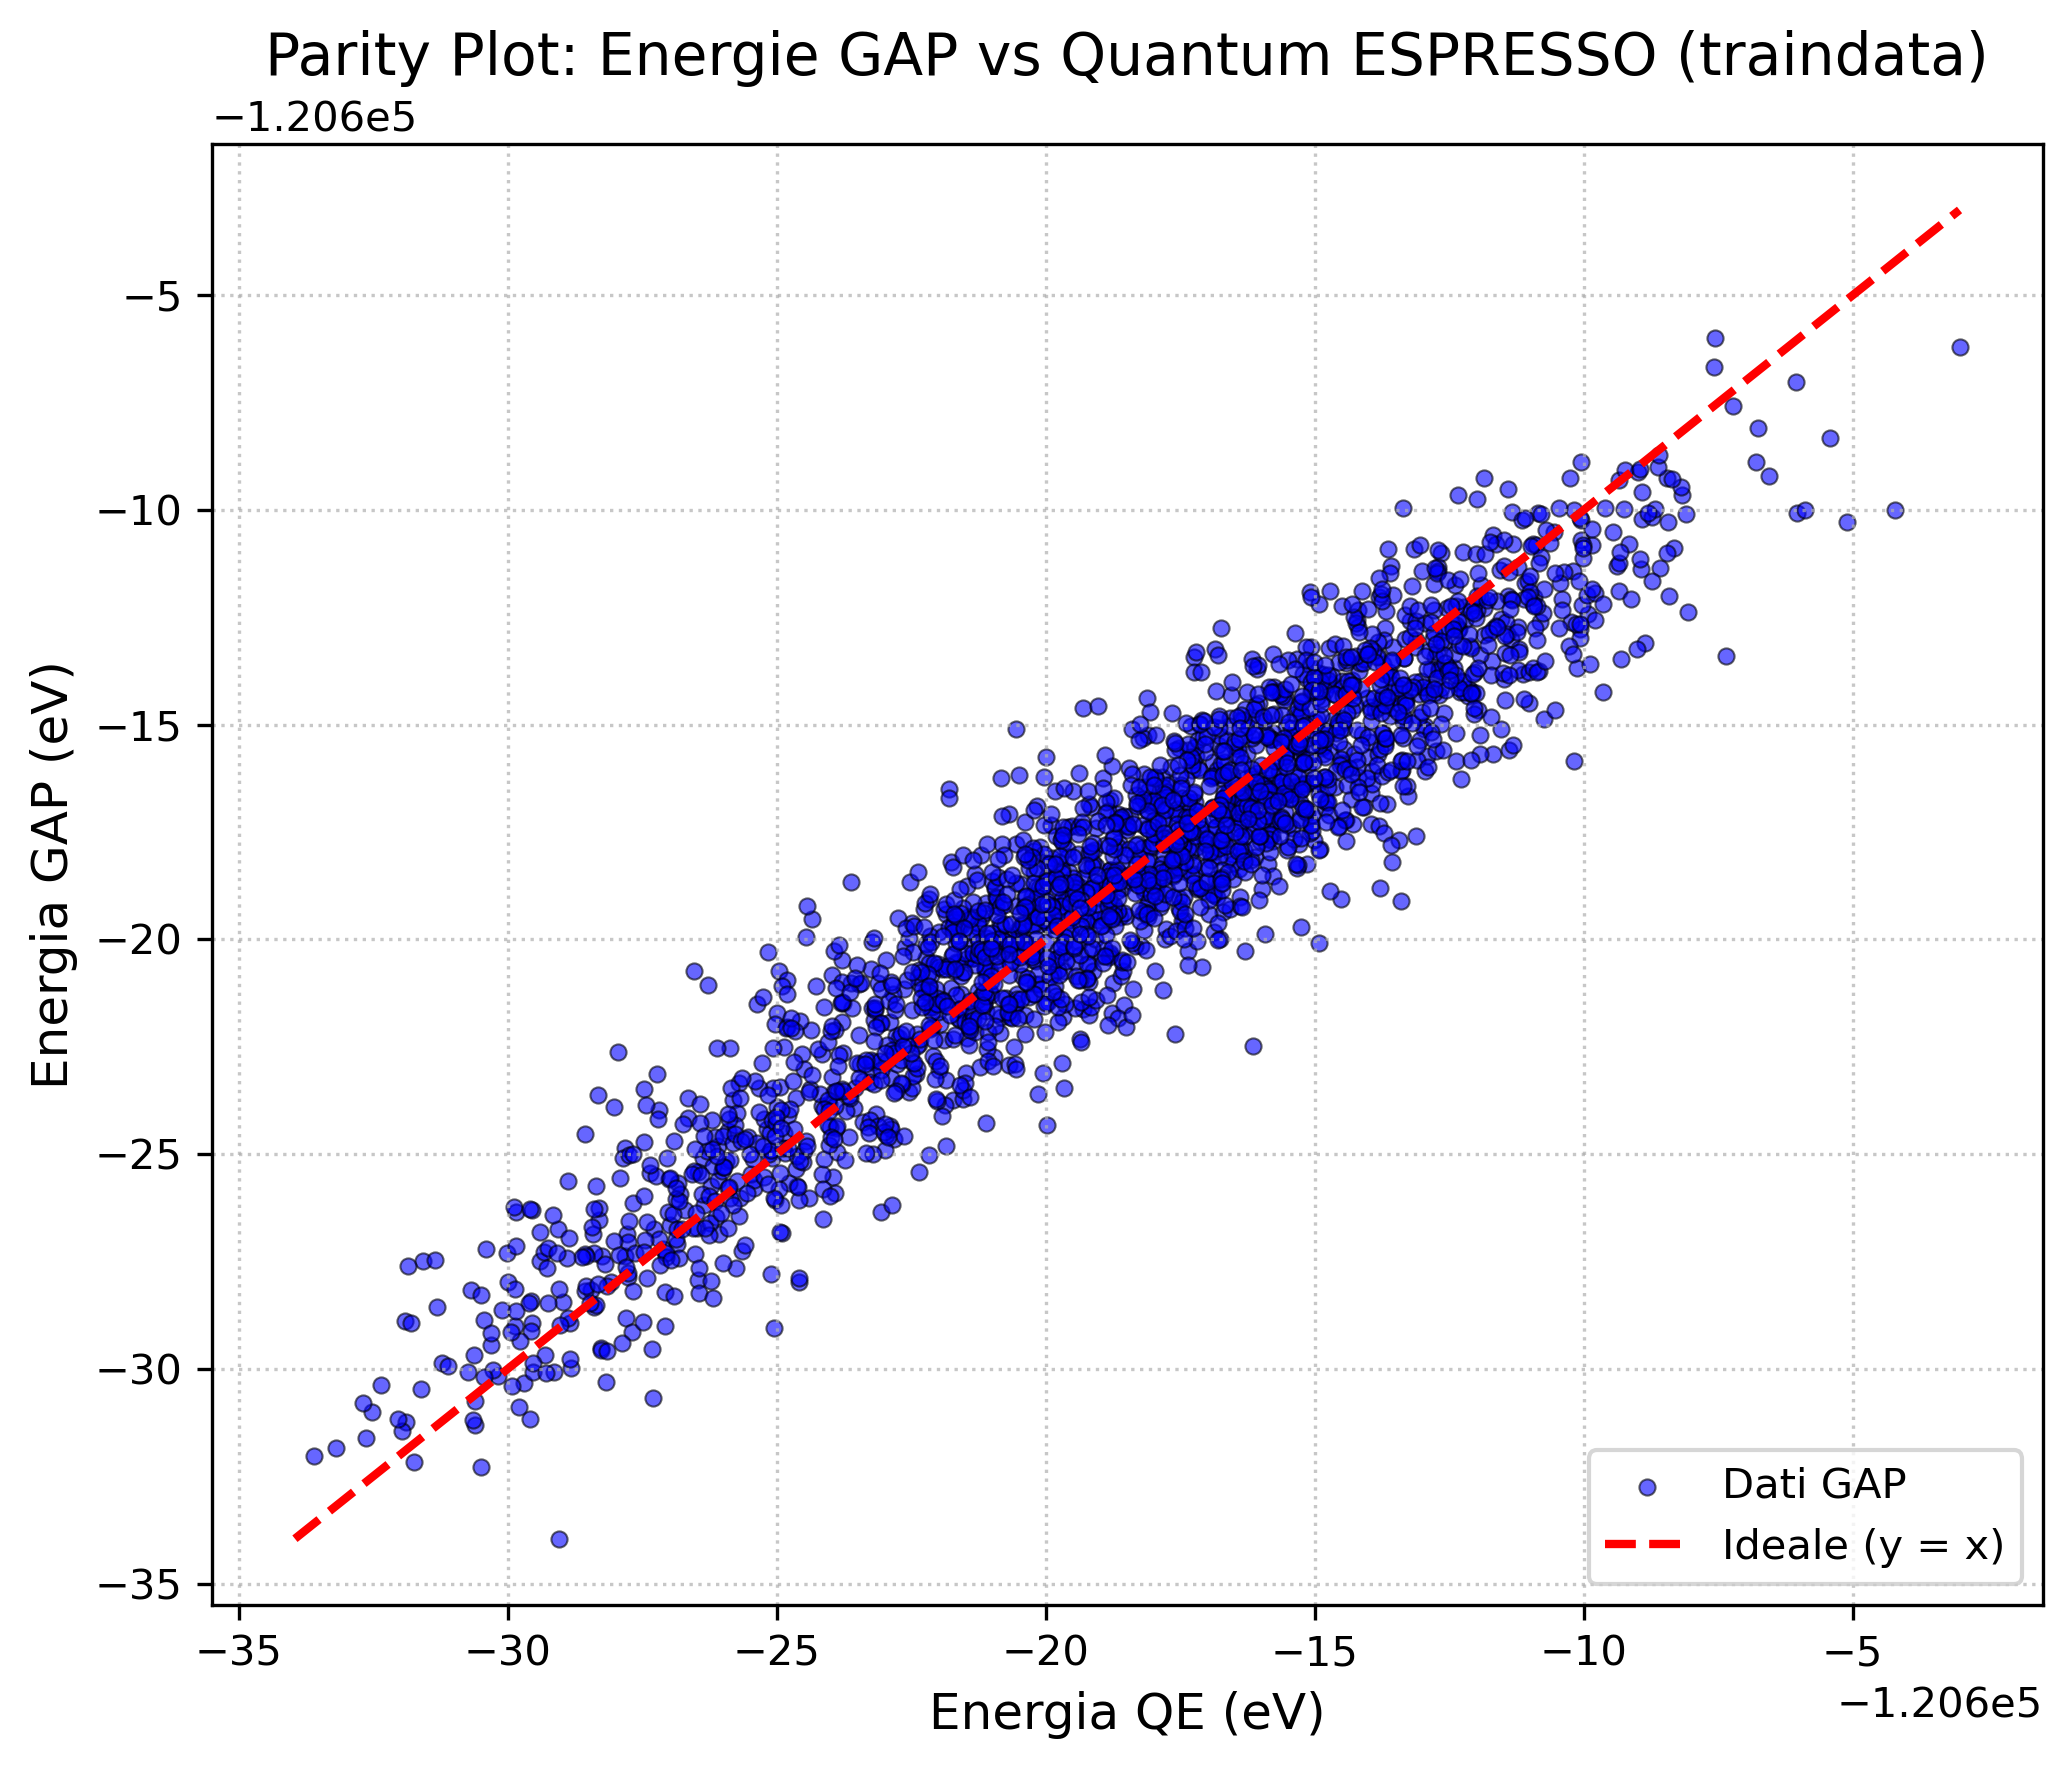
\includegraphics[scale=0.4]{./img/parity_plot_gap_vs_qe-traindata.png}
%    \caption{Confronto tra i valori di energia potenziale predetti dal potenziale GAP e quelli calcolati tramite Quantum Espresso}
%    \label{fig:parity_plot_gap_vs_qe-traindata}
%\end{figure}

Dal grafico (\ref{fig:parity_plot_gap_vs_qe-traindata}) possiamo osservare che il risultato è compatibile con le aspettative e le energie predette assomigliano a quelle calcolate da QE.


\subsubsection{Test set}

In questa fase, invece vogliamo verificare come si comporta il potenziale nel caso di dati su cui non è stato addestrato. Ricordiamo che questo set è composto dalla seconda metà della dinamica totale descritta dal dataset A.

%\begin{figure}[h]
%    \centering
%    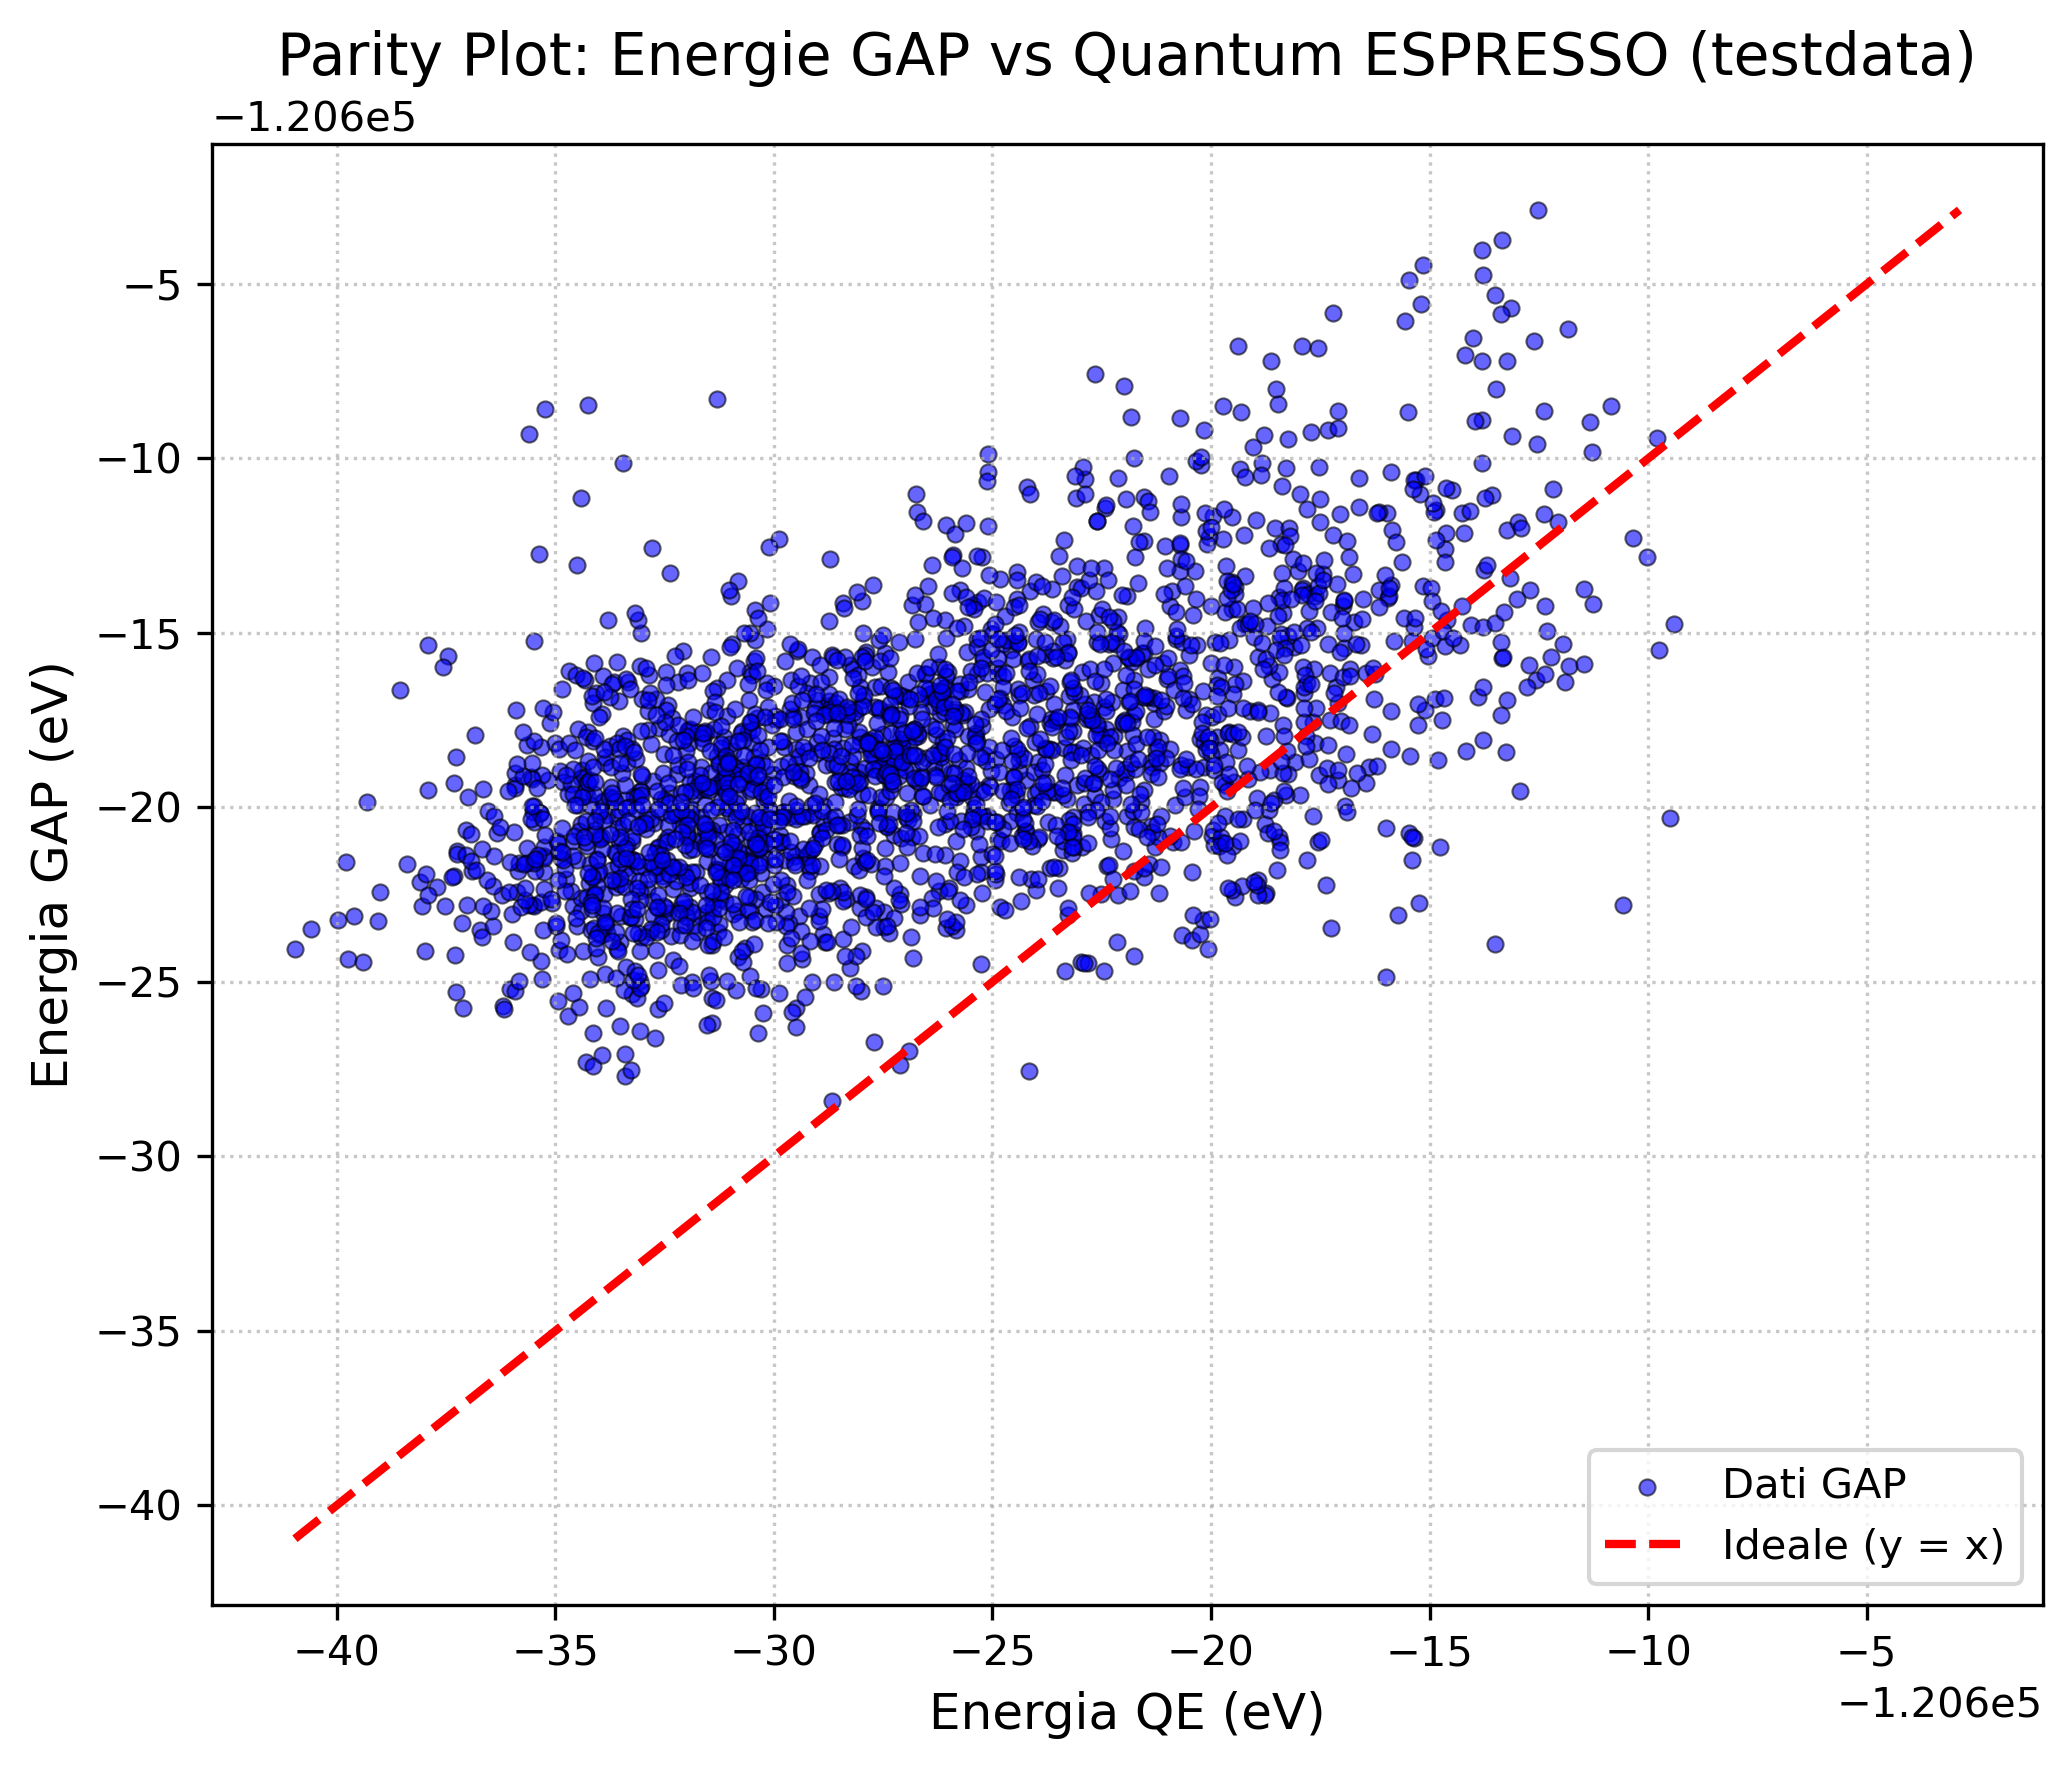
\includegraphics[scale=0.4]{./img/parity_plot_gap_vs_qe-testdata.png}
%    \caption{Confronto tra i valori di energia potenziale predetti dal potenziale GAP e quelli calcolati tramite Quantum Espresso}
%    \label{fig:parity_plot_gap_vs_qe-testdata}
%\end{figure}

Possiamo notare che i risultati in \autoref{fig:parity_plot_gap_vs_qe-testdata} non si allineano perfettamente con le aspettative, ma date le limitazioni dei parametri di addestramento del potenziale e dalla rapidità di calcolo ottenuta, possiamo considerare questo un buon risultato iniziale.


{
	\begin{figure}[ht]
		\centering
		\begin{subfigure}{0.45\textwidth}
		    \centering
    		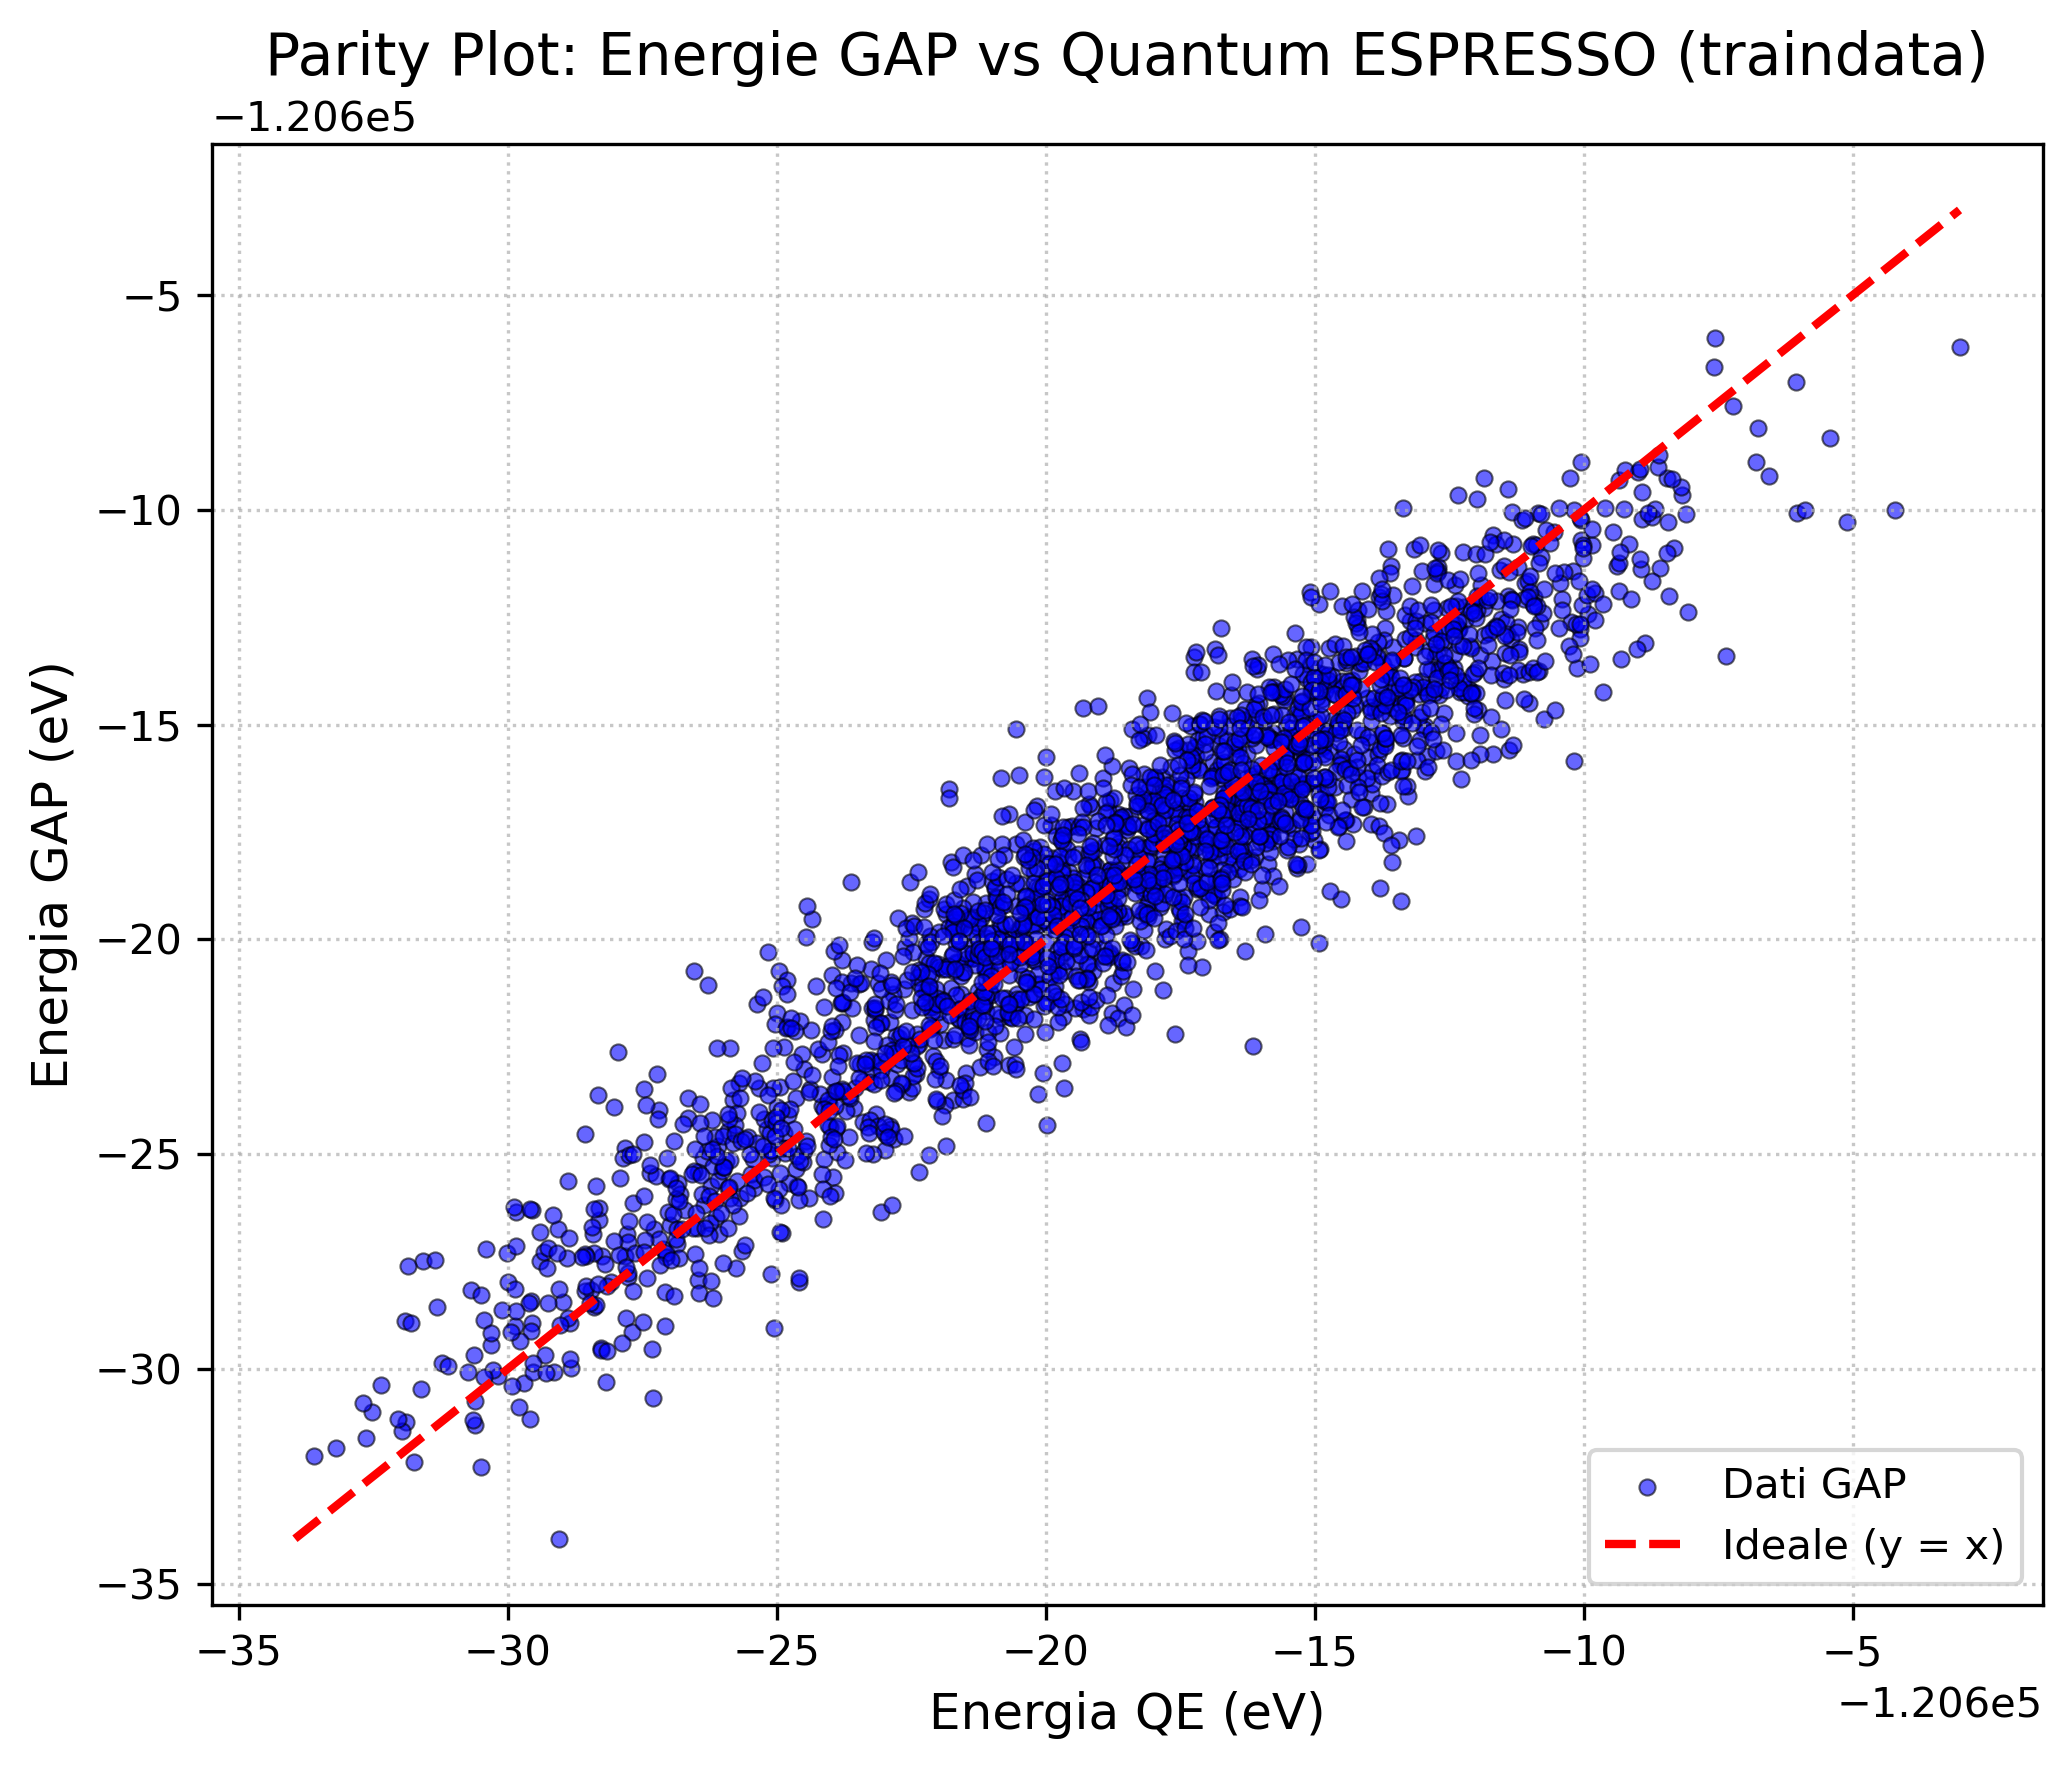
\includegraphics[scale=0.40]{./img/parity_plot_gap_vs_qe-traindata.png}
    		\caption{Confronto tra i valori di energia potenziale predetti dal potenziale GAP e quelli calcolati tramite Quantum Espresso}
    		\label{fig:parity_plot_gap_vs_qe-traindata}
		\end{subfigure}
		\hfill
		\begin{subfigure}{0.45\textwidth}
		    \centering
		    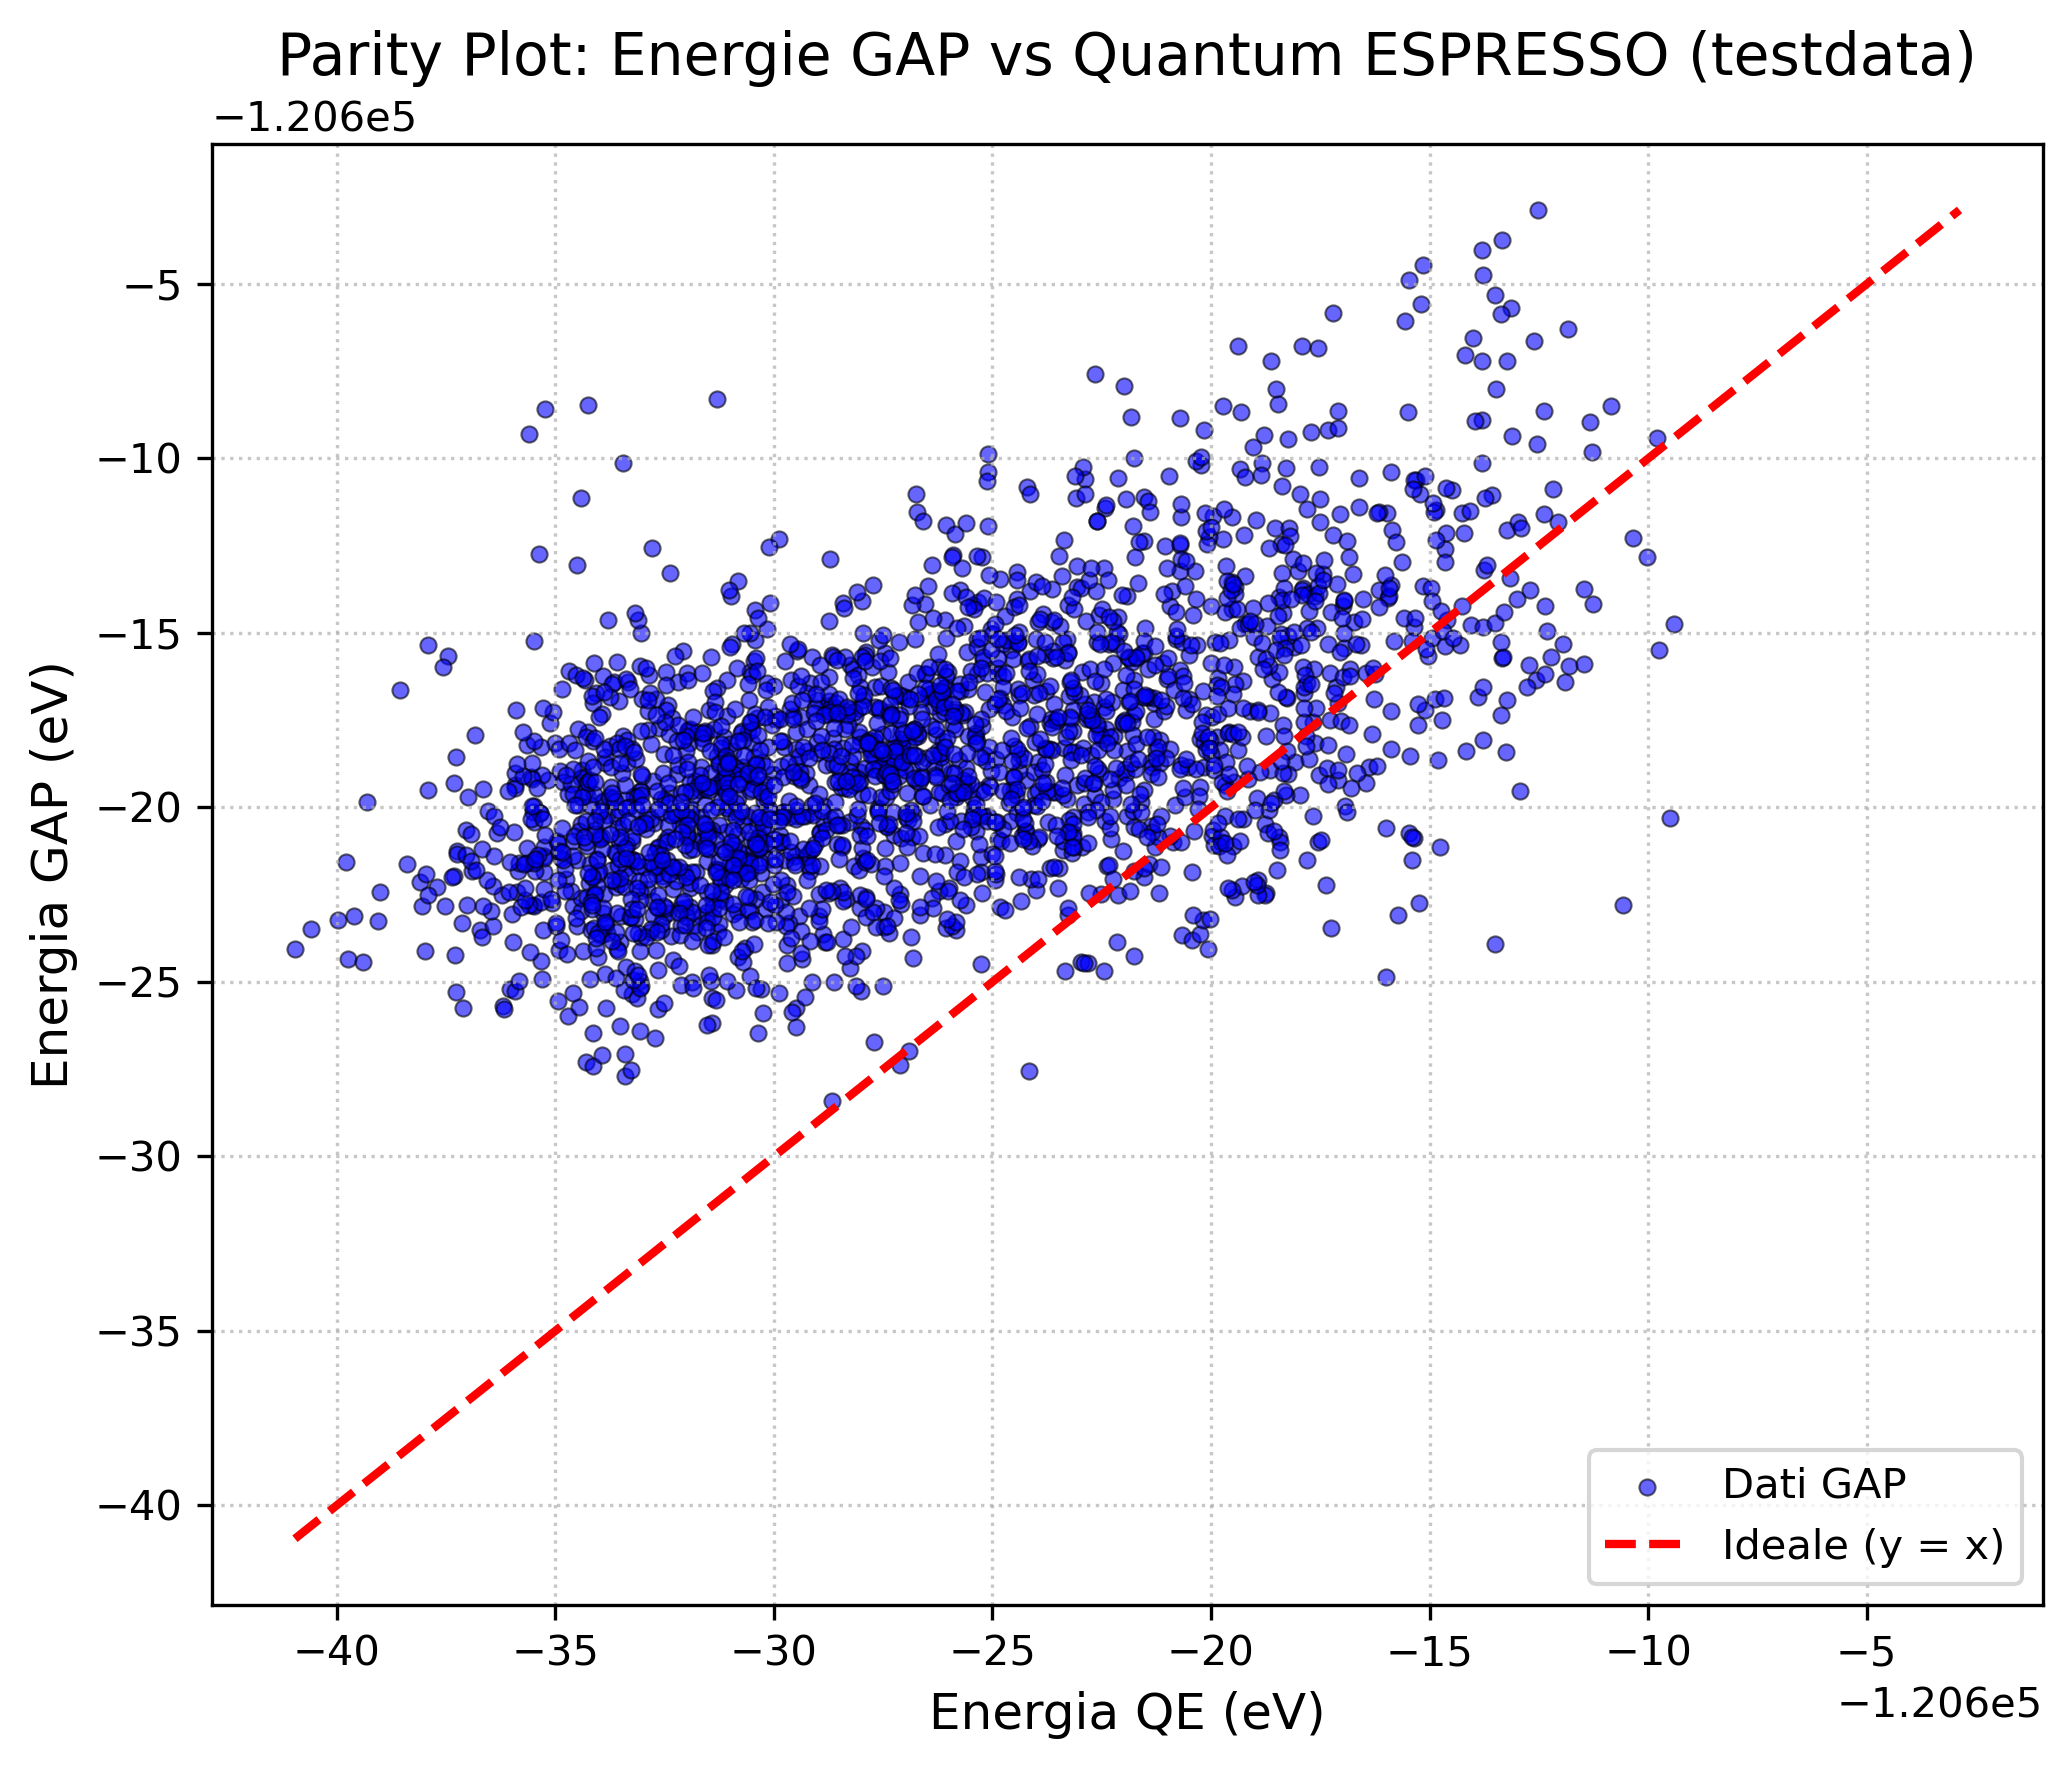
\includegraphics[scale=0.40]{./img/parity_plot_gap_vs_qe-testdata.png}
		    \caption{Confronto tra i valori di energia potenziale predetti dal potenziale GAP e quelli calcolati tramite Quantum Espresso}
    		\label{fig:parity_plot_gap_vs_qe-testdata}
		\end{subfigure}
		\label{fig:energie-test+train-set}
		\caption{Parity plot}
	\end{figure}
}



\subsection{Verifica delle forze}

Oltre a verificare le energie, abbiamo deciso di verificare anche le forze. Una volta estratte le forze da QE da usare come reference, abbiamo potuto determinare il valore delle forze usando il potenziale addestrato a partire dalle configurazioni usate da QE.

\subsubsection{Training set}

Il seguente grafico mostra il confronto tra le forze calcolate da QE e quelle predette dal potenziale, essendo queste le configurazioni usate nel training ci aspettiamo un buon accordo.

\begin{figure}[h]
    \centering
    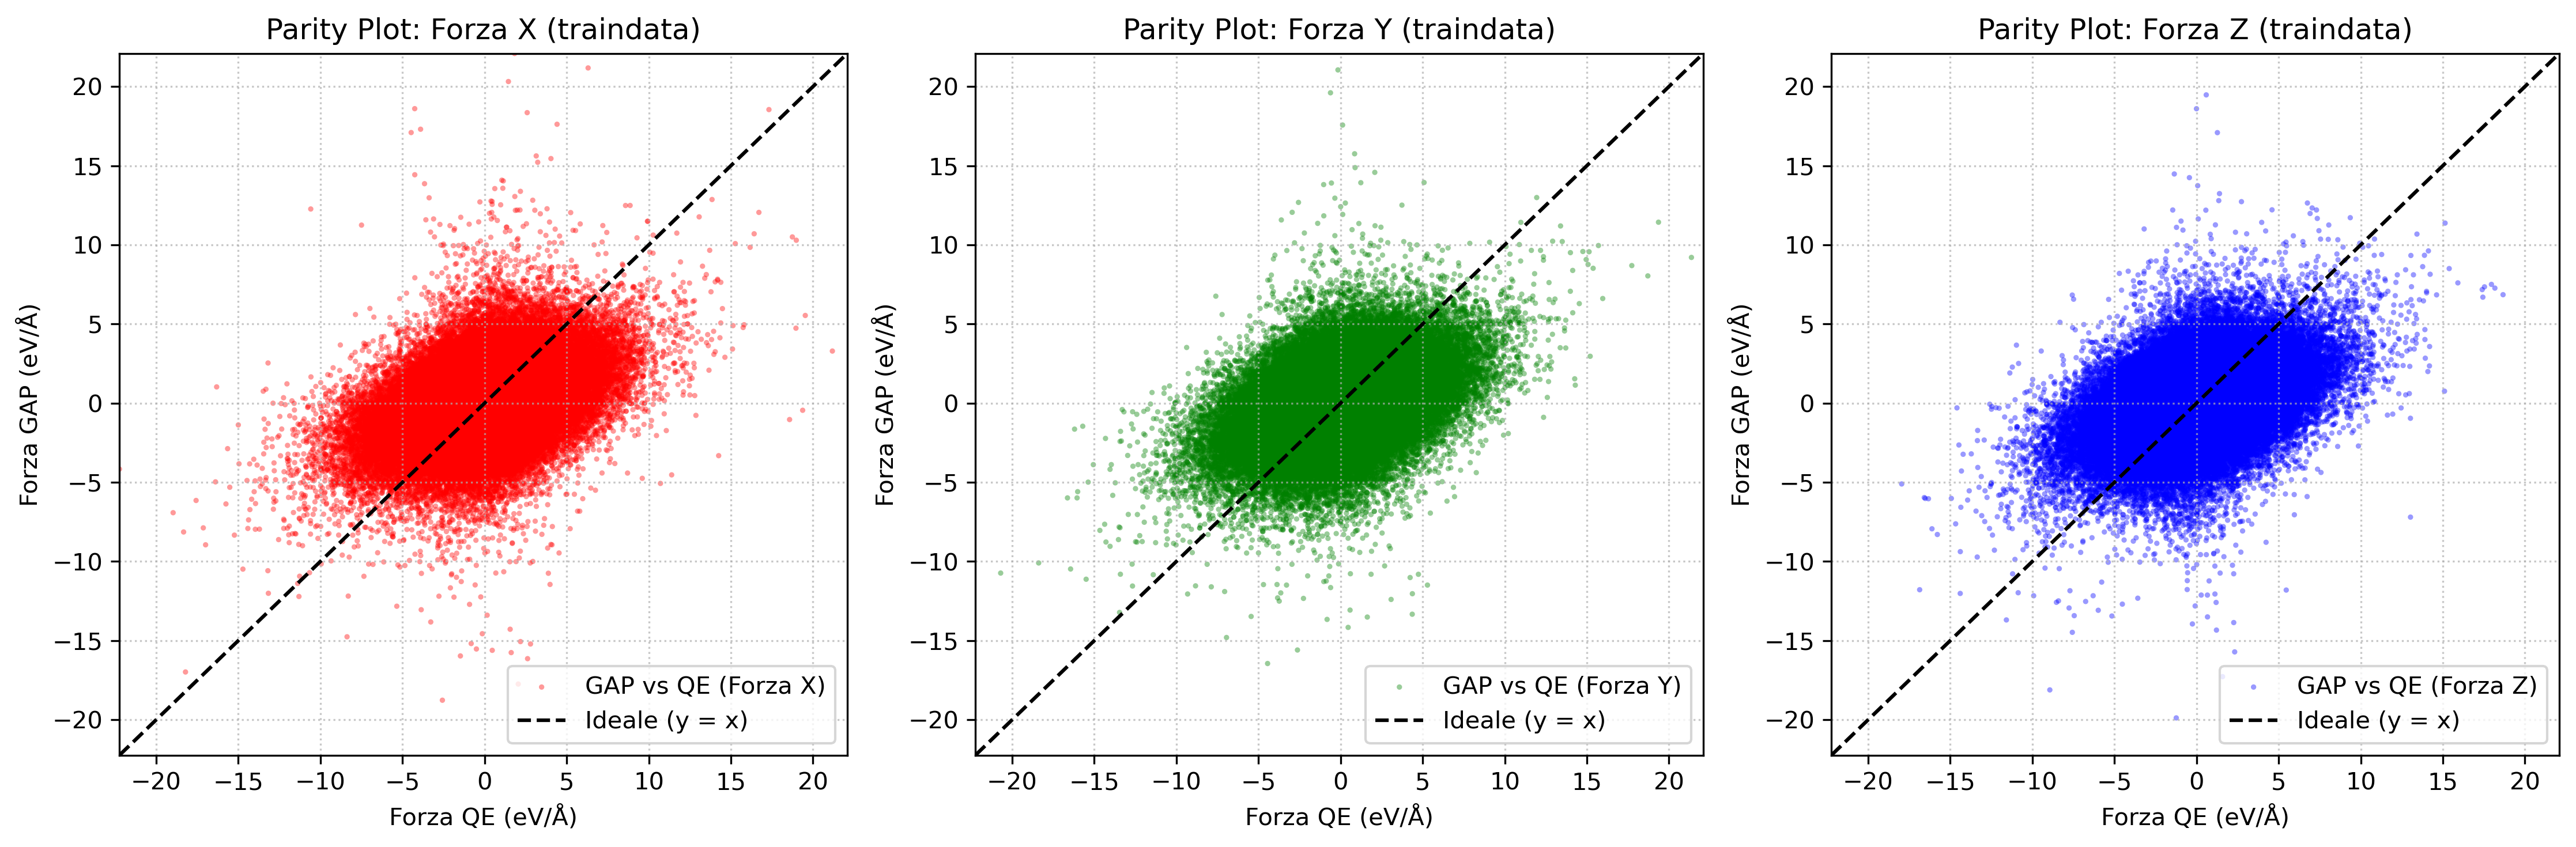
\includegraphics[scale=0.40]{./img/parity_plot_forze-traindata.png}
    \caption{Confronto, suddiviso per asse di riferimento, tra i valori di forza calcolati a partire da QE e dal potenziale addestrato.}
    \label{fig:parity_plot_forze-traindata}
\end{figure}


\subsubsection{Test set}

Procediamo adesso come sopra a utilizzare l'altra parte del dataset per verificare la compatibilità tra calcolo e predizioni.

\begin{figure}[h]
    \centering
    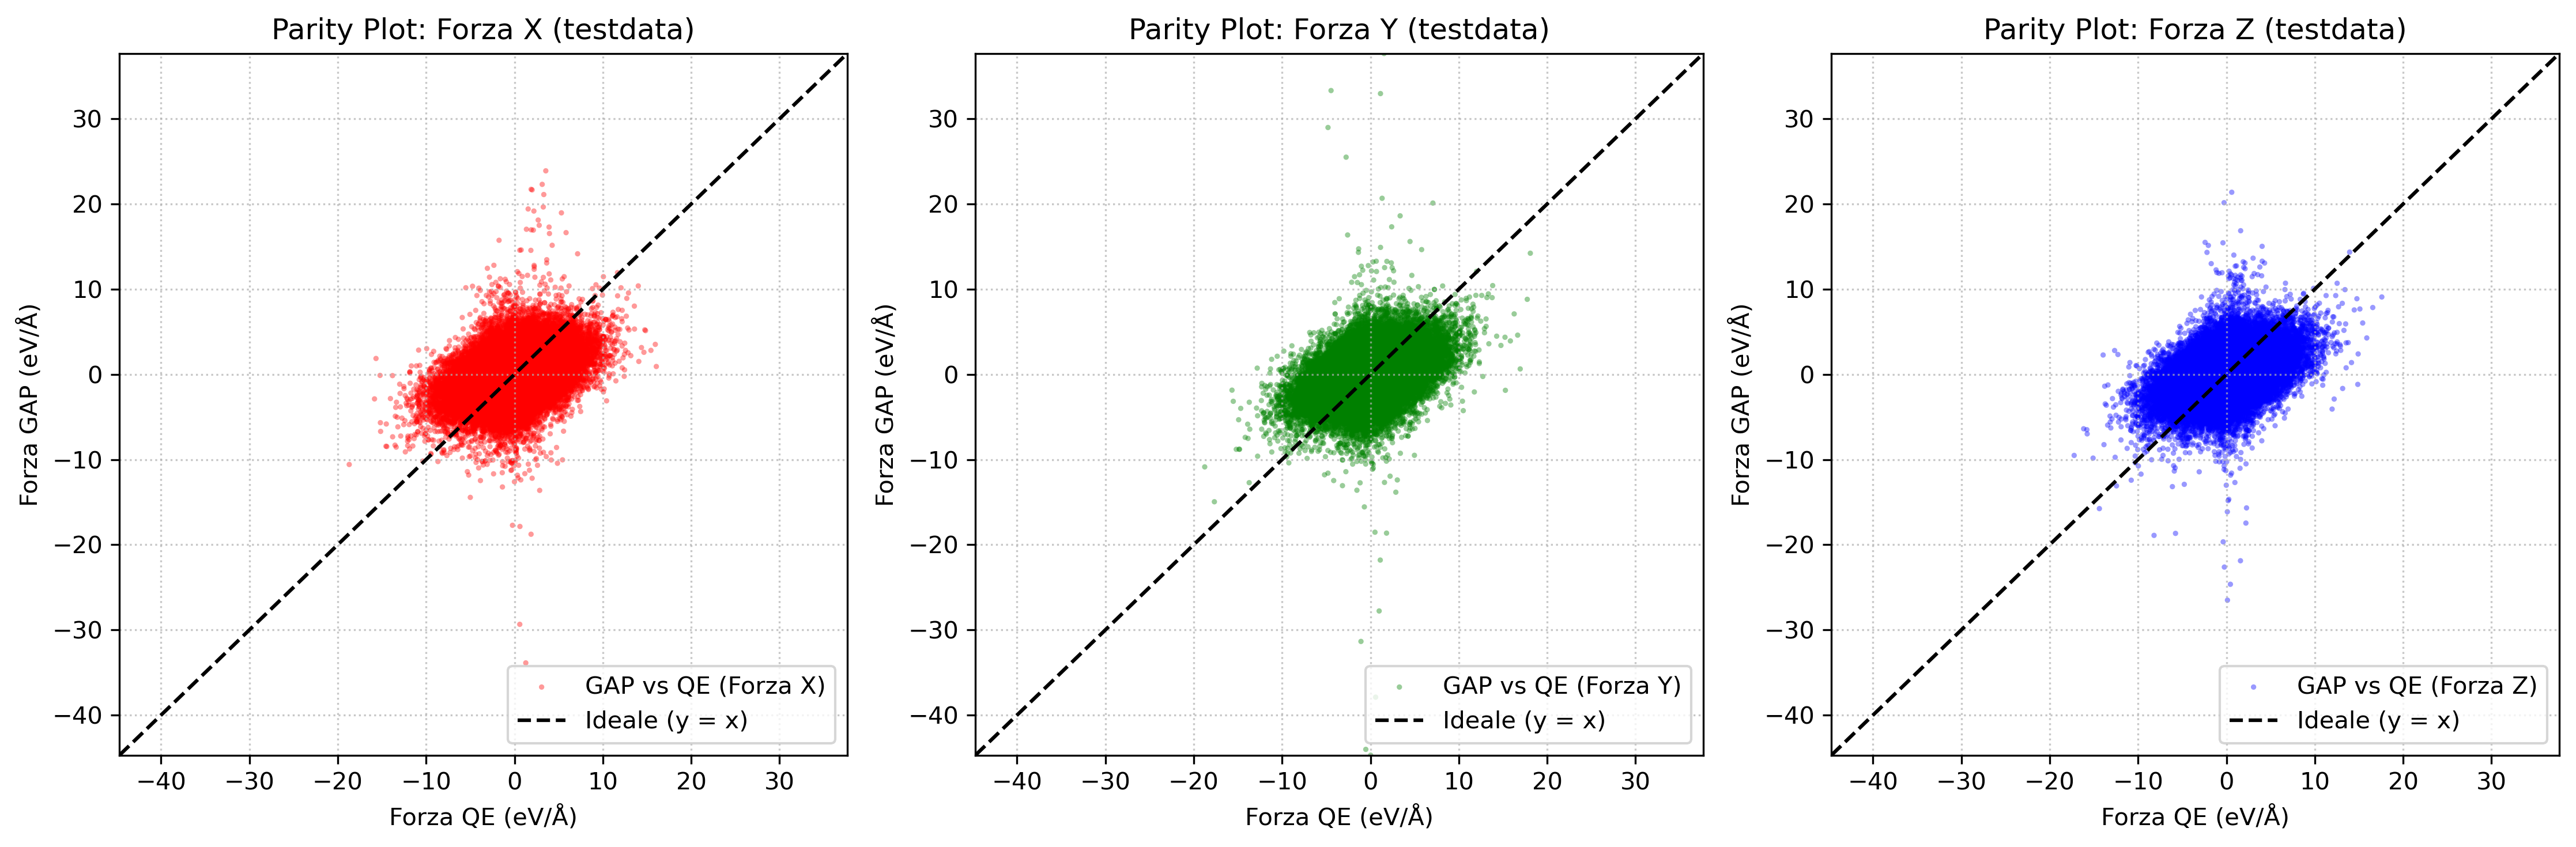
\includegraphics[scale=0.40]{./img/parity_plot_forze-testdata.png}
    \caption{Confronto, suddiviso per asse di riferimento, tra i valori di forza calcolati a partire da QE e dal potenziale addestrato}
    \label{fig:parity_plot_forze-testdata}
\end{figure}

Anche in questo caso i risultati mostrano un buon accordo.

Possiamo dunque ipotizzare che questo grado di accordo superiore rispetto alle energie, sia almeno in parte dovuto al fatto che l'errore stimato per le energie e inserito nei parametri di addestramento del potenziale, è di tre ordini di grandezza superiore.

    
    \chapter{Simulazione}
In questo capitolo ci occupiamo di utilizzare il potenziale ottenuto precedentemente per simulare il materiale in analisi.


\section{Simulazione NVE}

Abbiamo provato a effettuare una simulazione di tipo NVE, costruita nel seguente modo. Dai file di QE, per il set di test, abbiamo estratto la configurazione spaziale iniziale degli atomi.
Questa struttura è stata utilizzata come punto di partenza per il calcolo di energie e forze: la sua evoluzione darà poi configurazioni diverse rispetto a quelle prodotte da QE.
Seguendo la struttura descritta precedentemente è stata impostata la simulazione con i seguenti parametri: timestep pari a $4.8$ fs (come quello usato in QE) e un totale di $2'000$ step.
Come detto, data la diversa configurazione, i risultati non possono essere confrontati direttamente con quelli prodotti da QE. 
Per verificare la stabilità dei risultati facciamo un grafico della temperatura e dell'energia in funzione dello step temporale.
Si è provato a reperire i valori delle velocità iniziali dal file di output di QE, ma non essendo presenti, le abbiamo estratte da una distribuzione di Maxwell-Boltzmann per una temperatura di $3'000$ K.
\\

I risultati di energia e temperatura che otteniamo sono in \autoref{fig:andamento_nve-testdata}:

\begin{figure}[h]
    \centering
    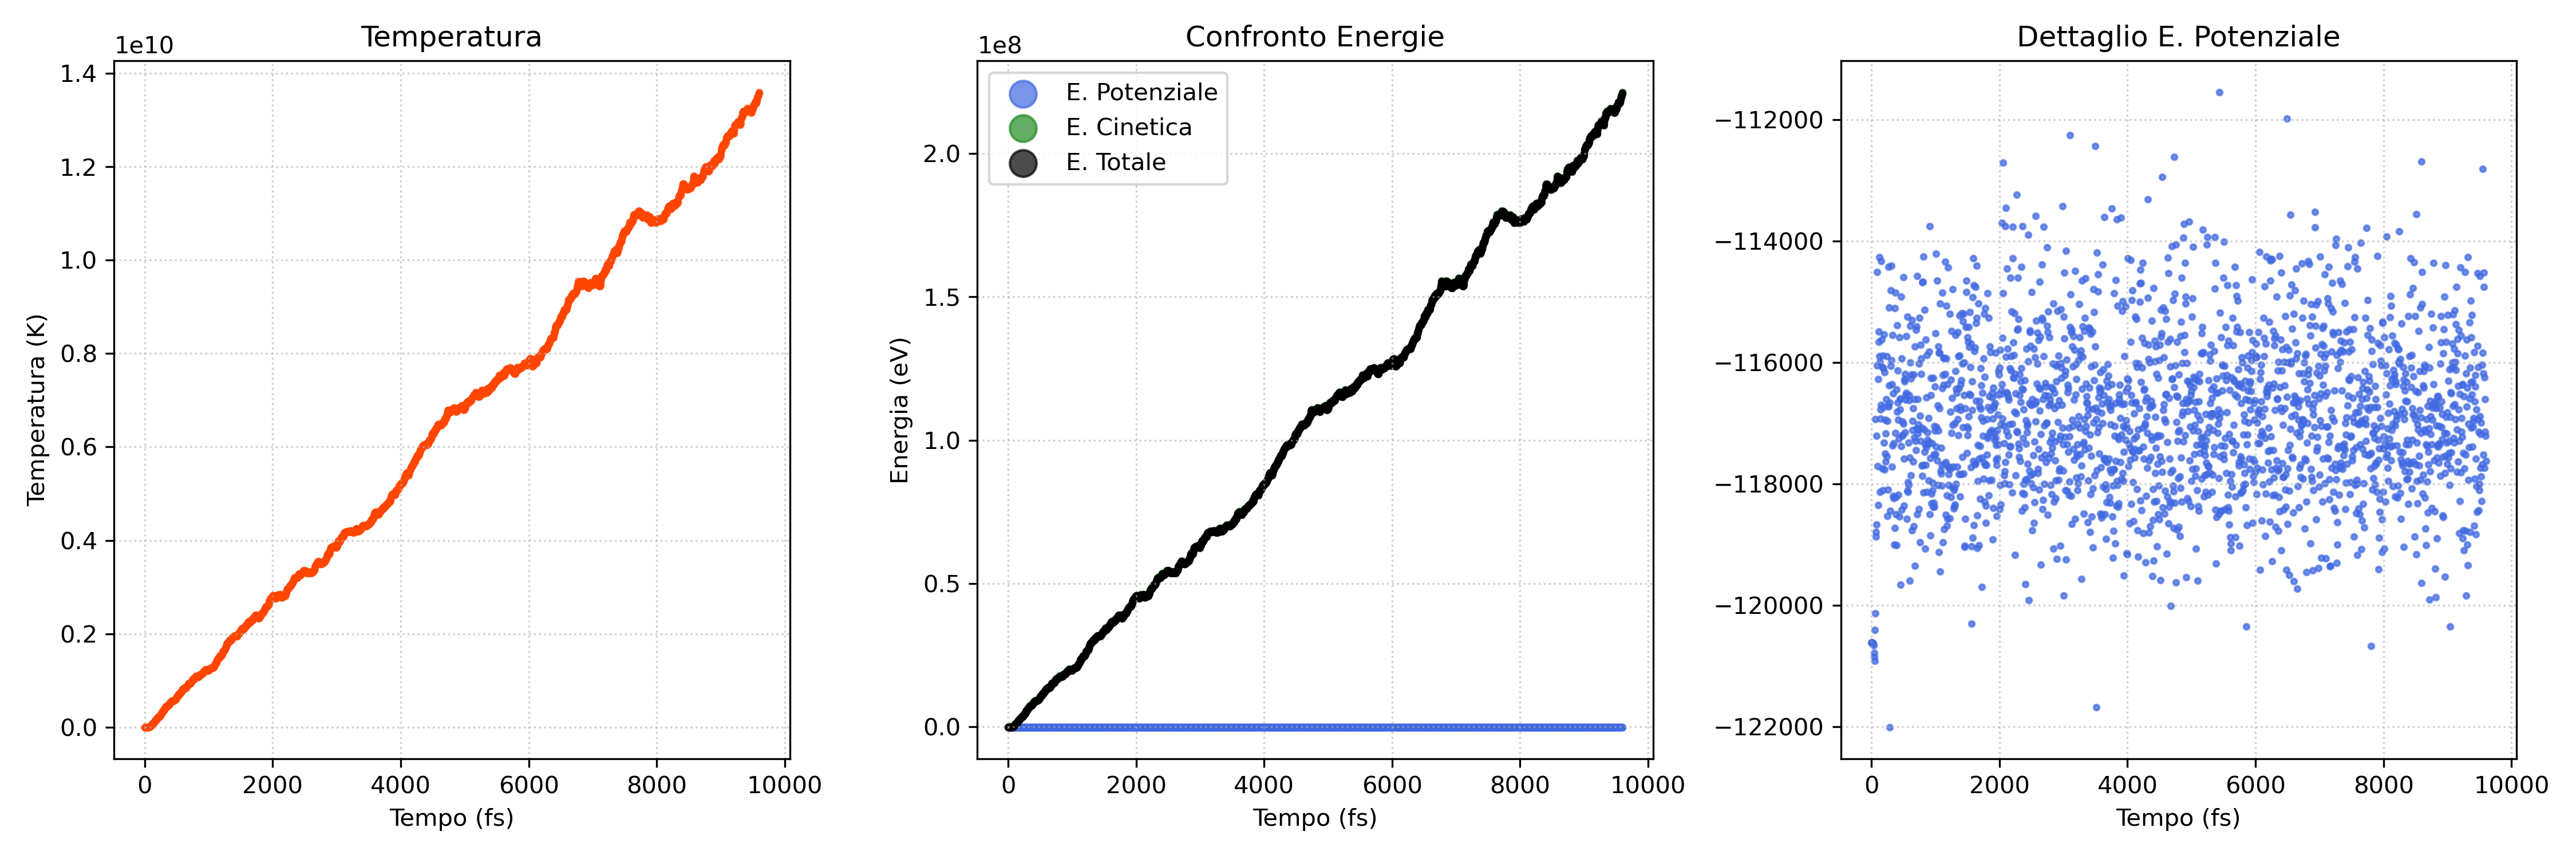
\includegraphics[scale=0.40]{./img/andamento_energia_nve_testdata.png}
    \caption{Grafico dell'andamento temporale per i valori di energia e temperatura.}
    \label{fig:andamento_nve-testdata}
\end{figure}

possiamo notare in \autoref{fig:andamento_nve-testdata} che i valori di energia e temperatura divergono a valori fisicamente insensati.
L'energia potenziale oscilla entro valori limite, osserviamo comunque che l'intervallo di oscillazione è relativamente ampio.

Risulta utile anche guardare ai valori di forza associati a questa dinamica, riportati nel grafico (\ref{fig:andamento_nve_forze-testdata}), dove anche in questo caso possiamo notare che otteniamo valori estremamente elevati.

\begin{figure}[h]
    \centering
    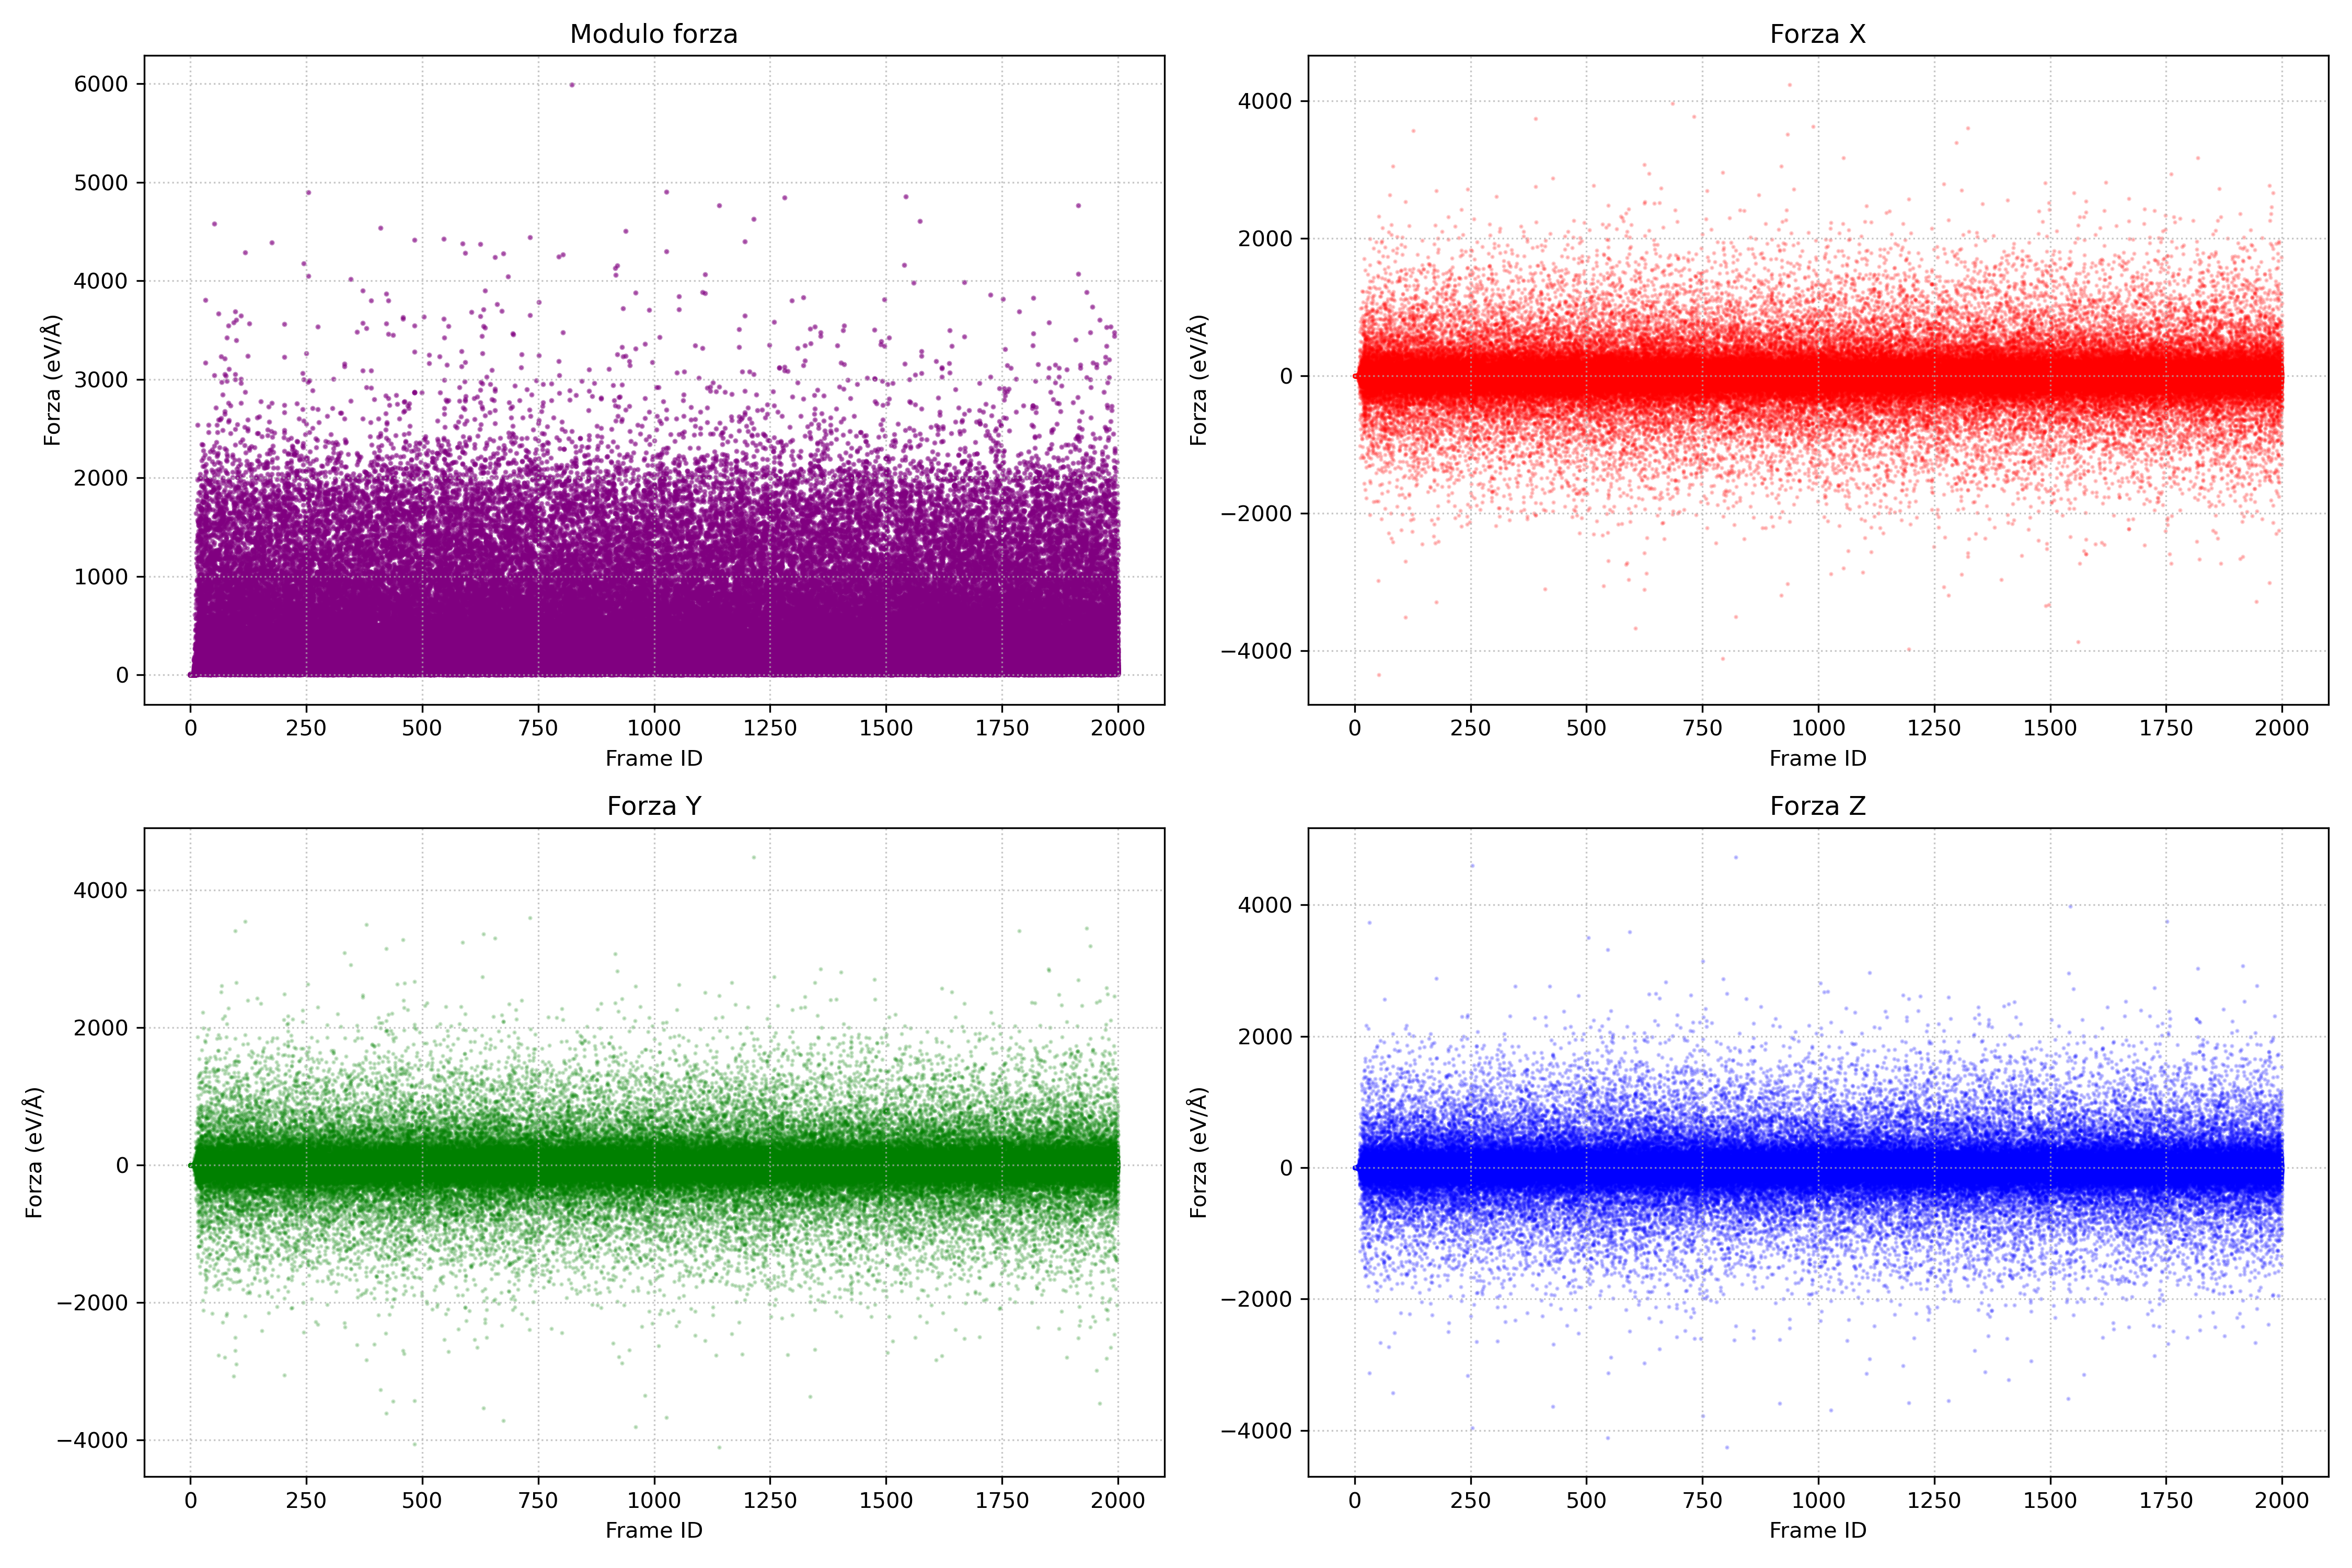
\includegraphics[scale=0.40]{./img/andamento_forze_totali_blocchi_nve_testdata.png}
    \caption{Grafico dell'andamento temporale per i valori di forza, sia in modulo che divise per componenti. }
    \label{fig:andamento_nve_forze-testdata}
\end{figure}


\section{Analisi delle problematiche} %--------------------------------------------------------------------------------------------------------------------------------------------------------------------------------------------------------

In precedenza si è menzionato che il potenziale è stato addestrato con parametri di SOAP non troppo elevati. Poniamo questo come ultimo problema da verificare, in quanto, i risultati sulle configurazioni di test erano discreti.
In questa sezione ci proponiamo di modificare a turno vari parametri, o combinazioni degli stessi, in modo da poter identificare quale sia il problema.


\subsection{Temperatura}

Come primo test abbiamo provato a modificare la temperatura dalla quale venivano estratti i valori di velocità. 
Si è impostato questo valore a $0$ K, mentre gli altri parametri sono rimasti invariati. 
Anche in questo caso diamo sia i risultati per i valori di energia sia di temperatura \autoref{fig:andamento_nve-traindata_0k}:

\begin{figure}[h]
    \centering
    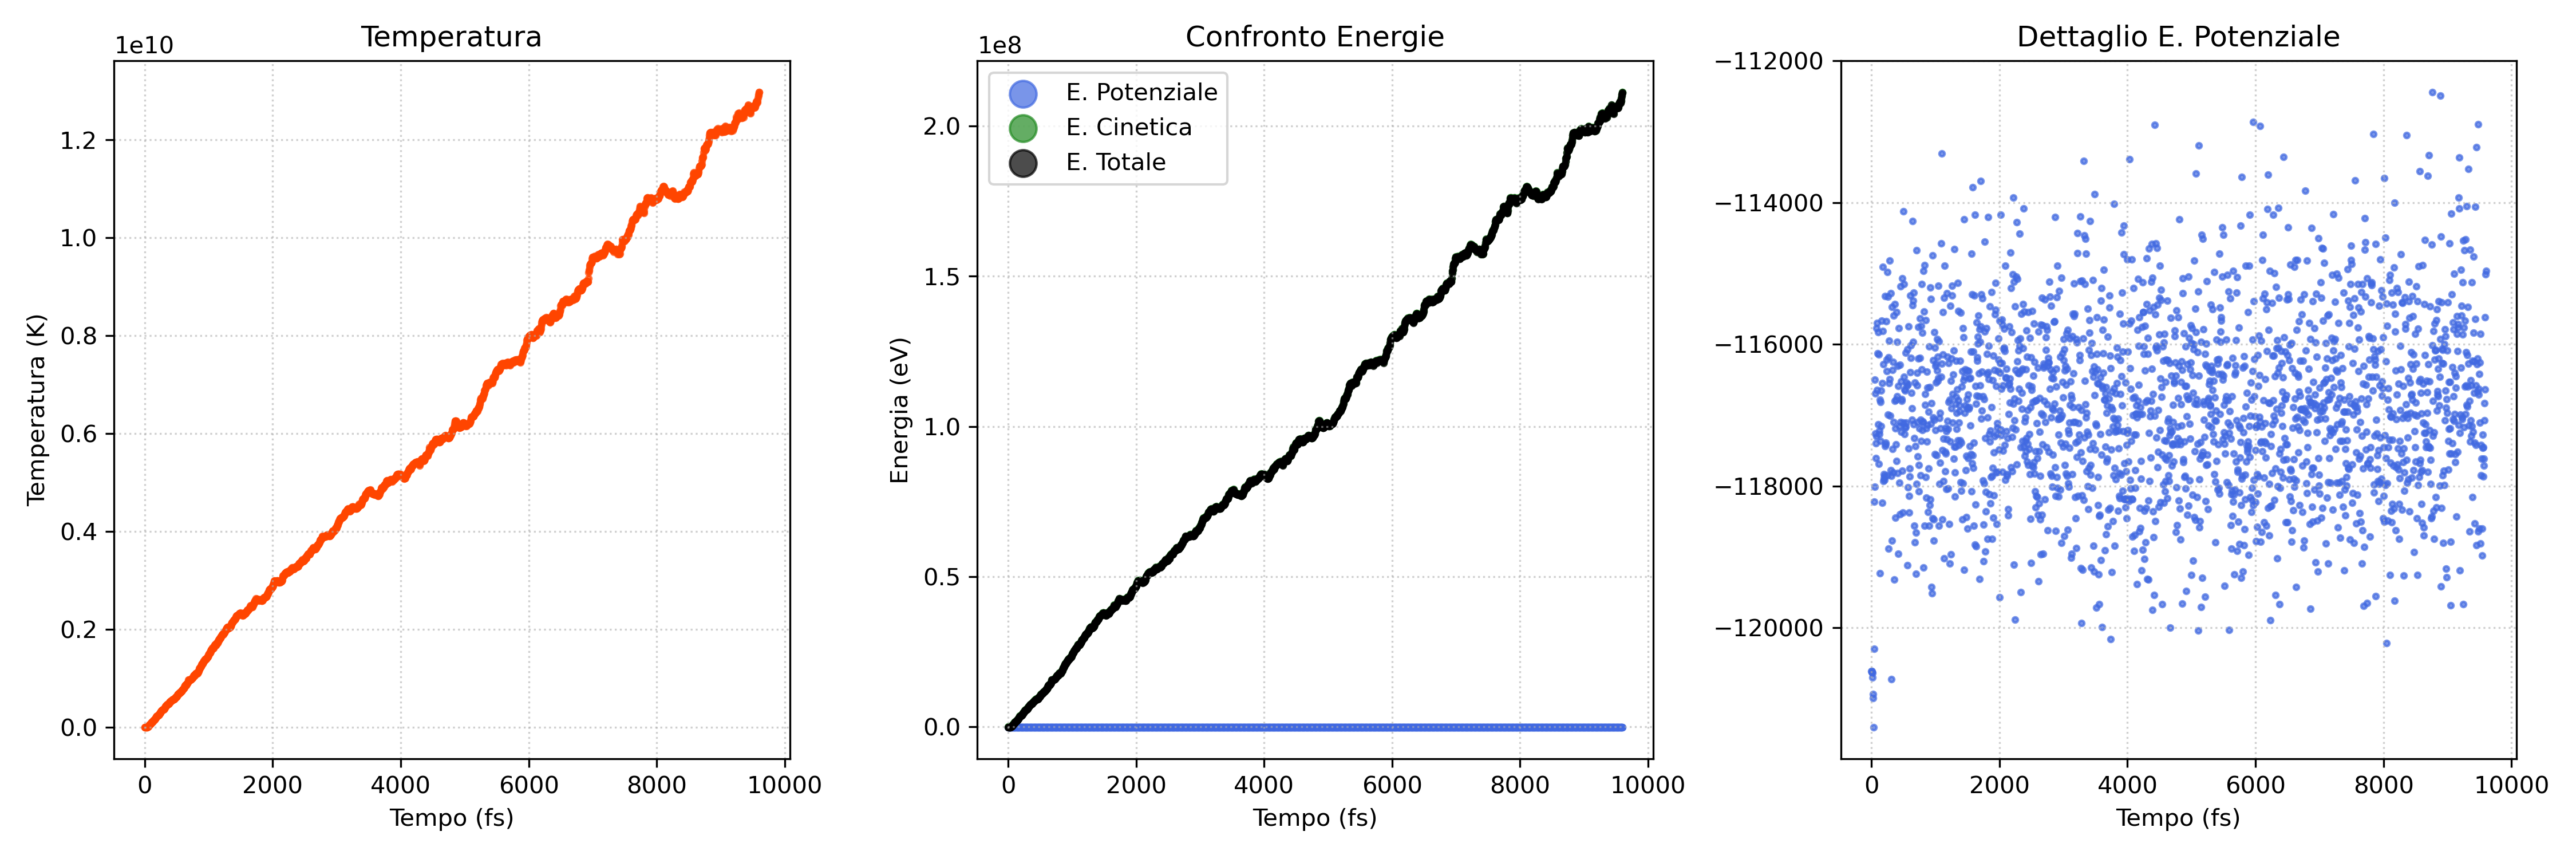
\includegraphics[scale=0.40]{./img/andamento_energia_nve_testdata_0k.png}
    \caption{Grafico dell'andamento temporale per i valori di energia e temperatura}
    \label{fig:andamento_nve-traindata_0k}
\end{figure}


che per i valori delle forze in \autoref{fig:andamento_nve_forze-traindata_0k}.

\begin{figure}[h]
    \centering
    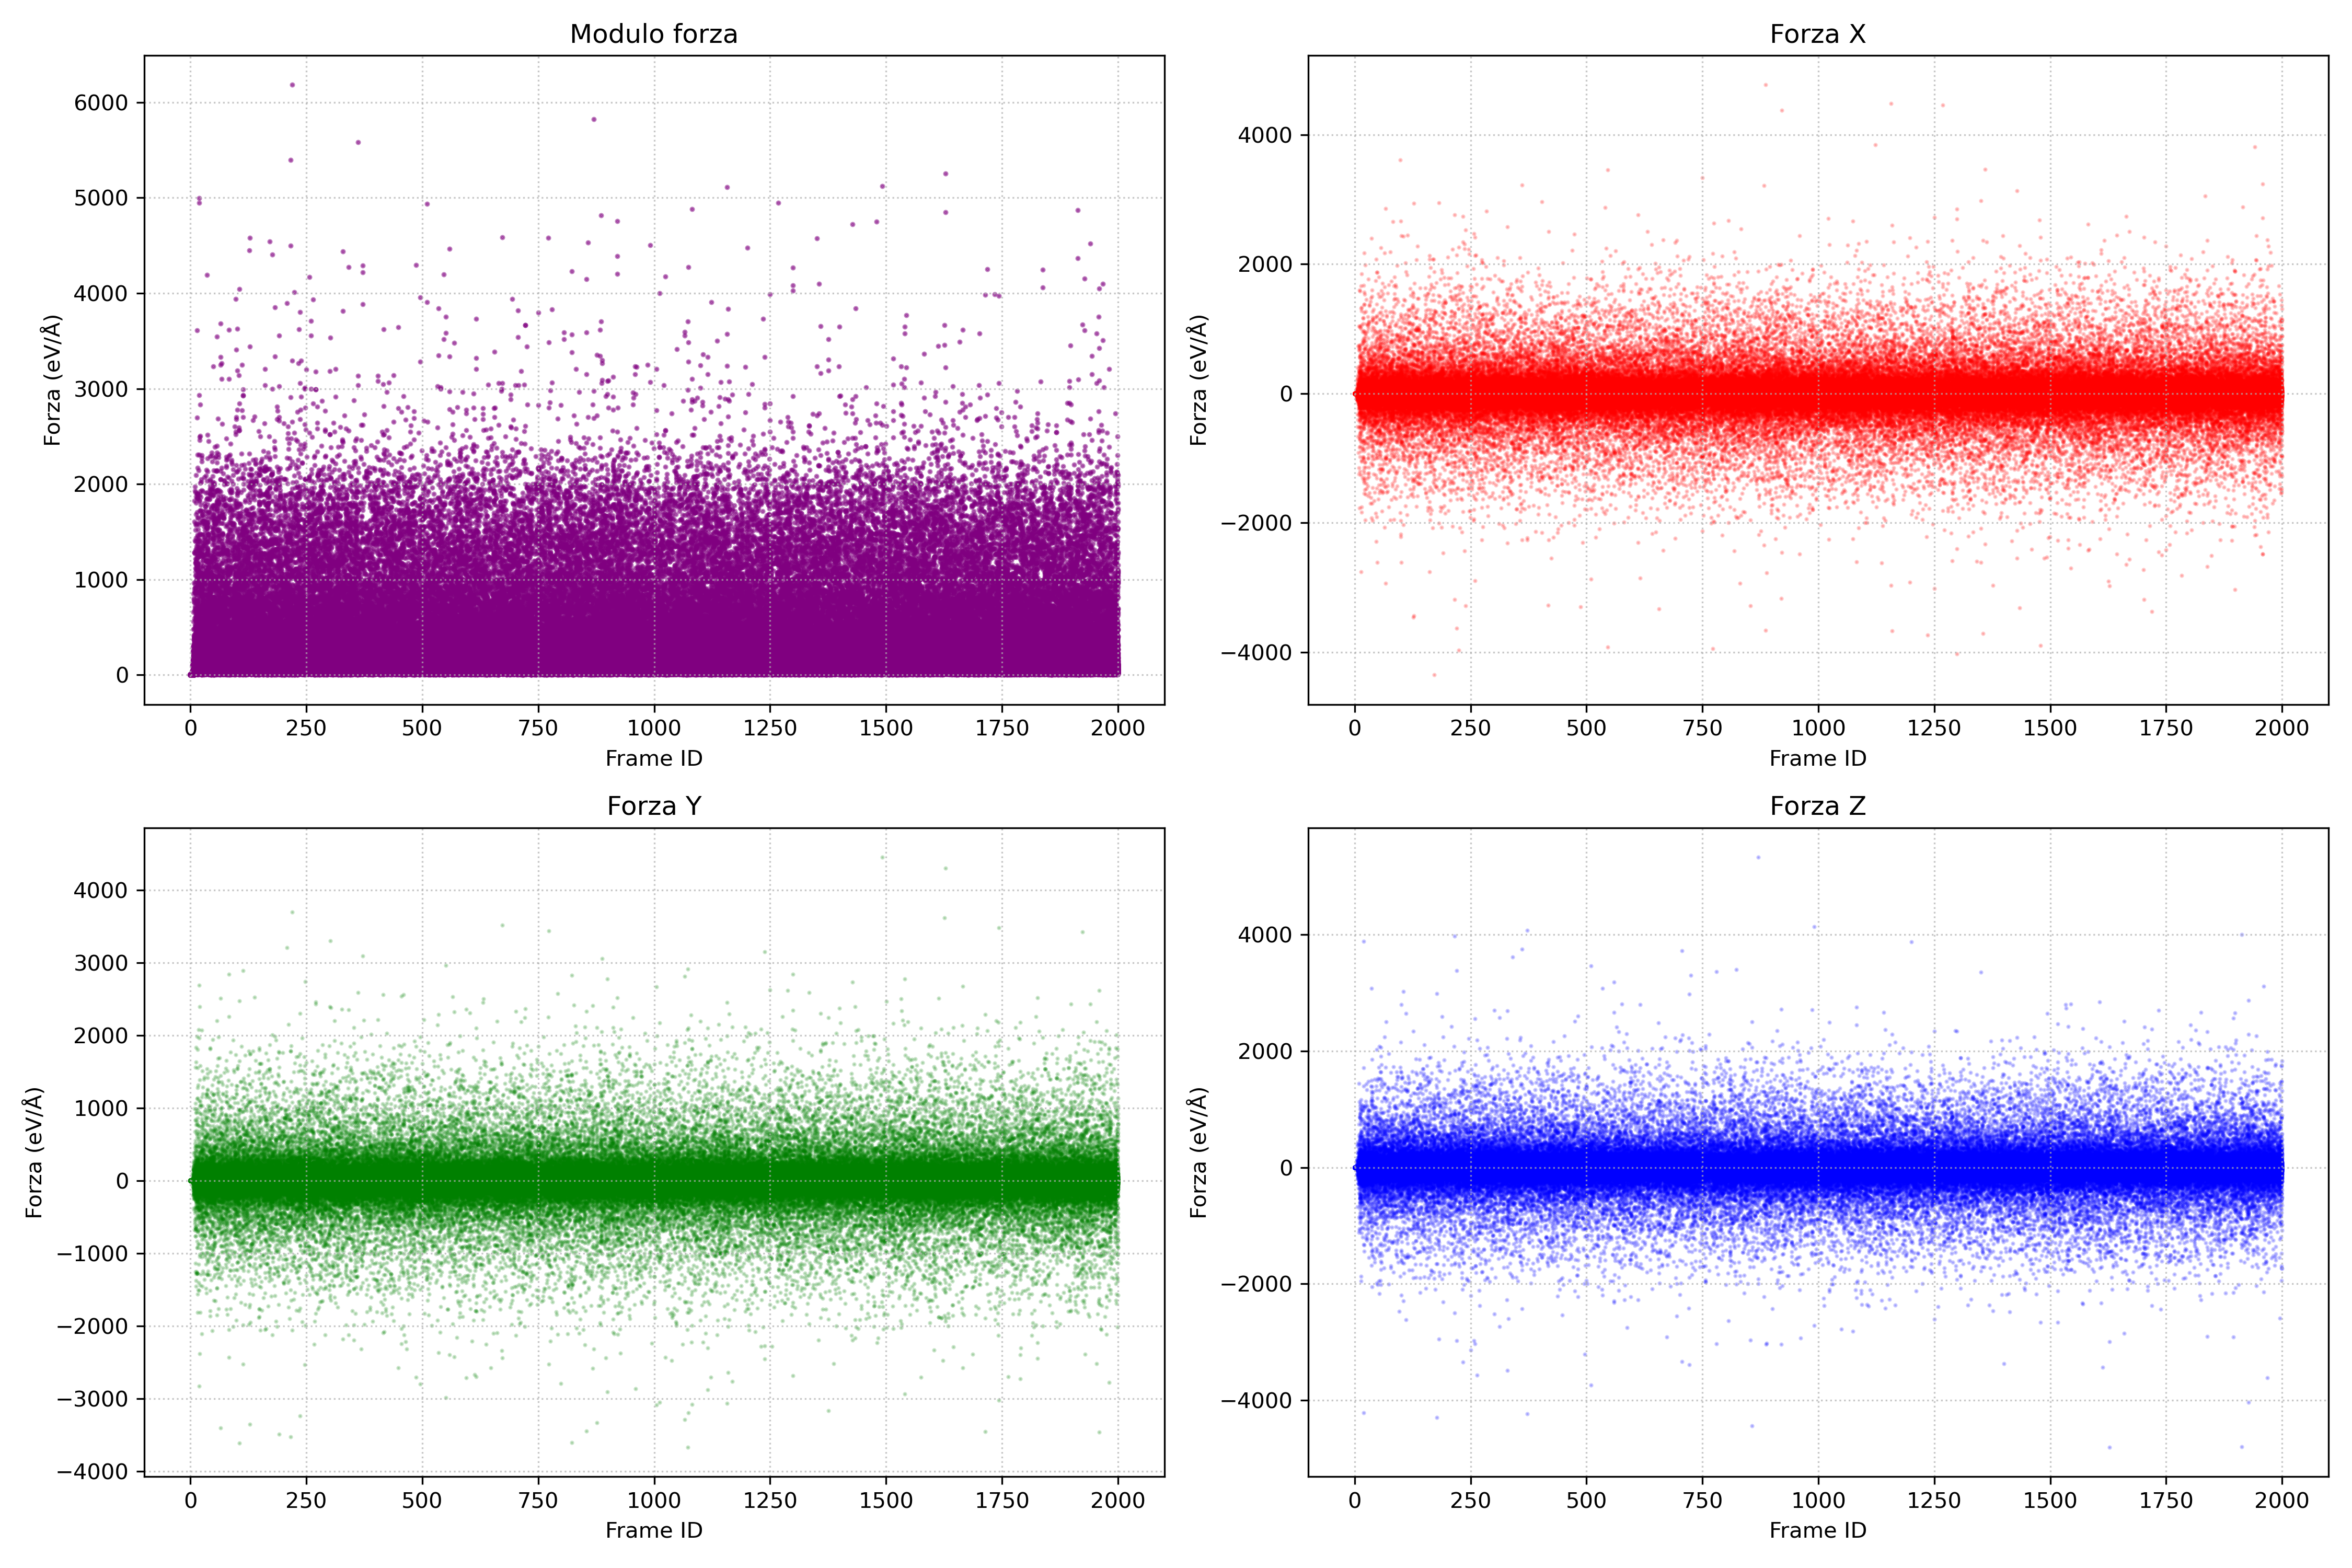
\includegraphics[scale=0.40]{./img/andamento_forze_totali_blocchi_nve_testdata_0k.png}
    \caption{Grafico dell'andamento temporale per i valori di forza, sia in modulo che divise per componenti. }
    \label{fig:andamento_nve_forze-traindata_0k}
\end{figure}

Si nota in \autoref{fig:andamento_nve-traindata_0k} e in \autoref{fig:andamento_nve_forze-traindata_0k}, che il risultato non è dissimile da quello ottenuto in precedenza, possiamo quindi escludere che sia un problema legato al valore di temperatura.



\subsection{Timestep} %----------------------------------------------------------------------------------------------------------------------------------------------------------------------------------------------------------------------

Per questa analisi sono stati provati diversi valori di timestep, riportiamo solo uno di questi.
Come timestep si è impostato un valore di $10^{-5}$ fs, e un totale di $50'000$ iterazioni, in modo da valutare la stabilità sul lungo periodo. Si è mantenuta una temperatura di $3'000$ K.

I valori di energia e temperatura sono rappresentati nel grafico (\ref{fig:andamento_nve_energie_timestep}), mentre per quanto riguarda le forze otteniamo il grafico (\ref{fig:andamento_nve_forze_timestep}).

\begin{figure}[h]
    \centering
    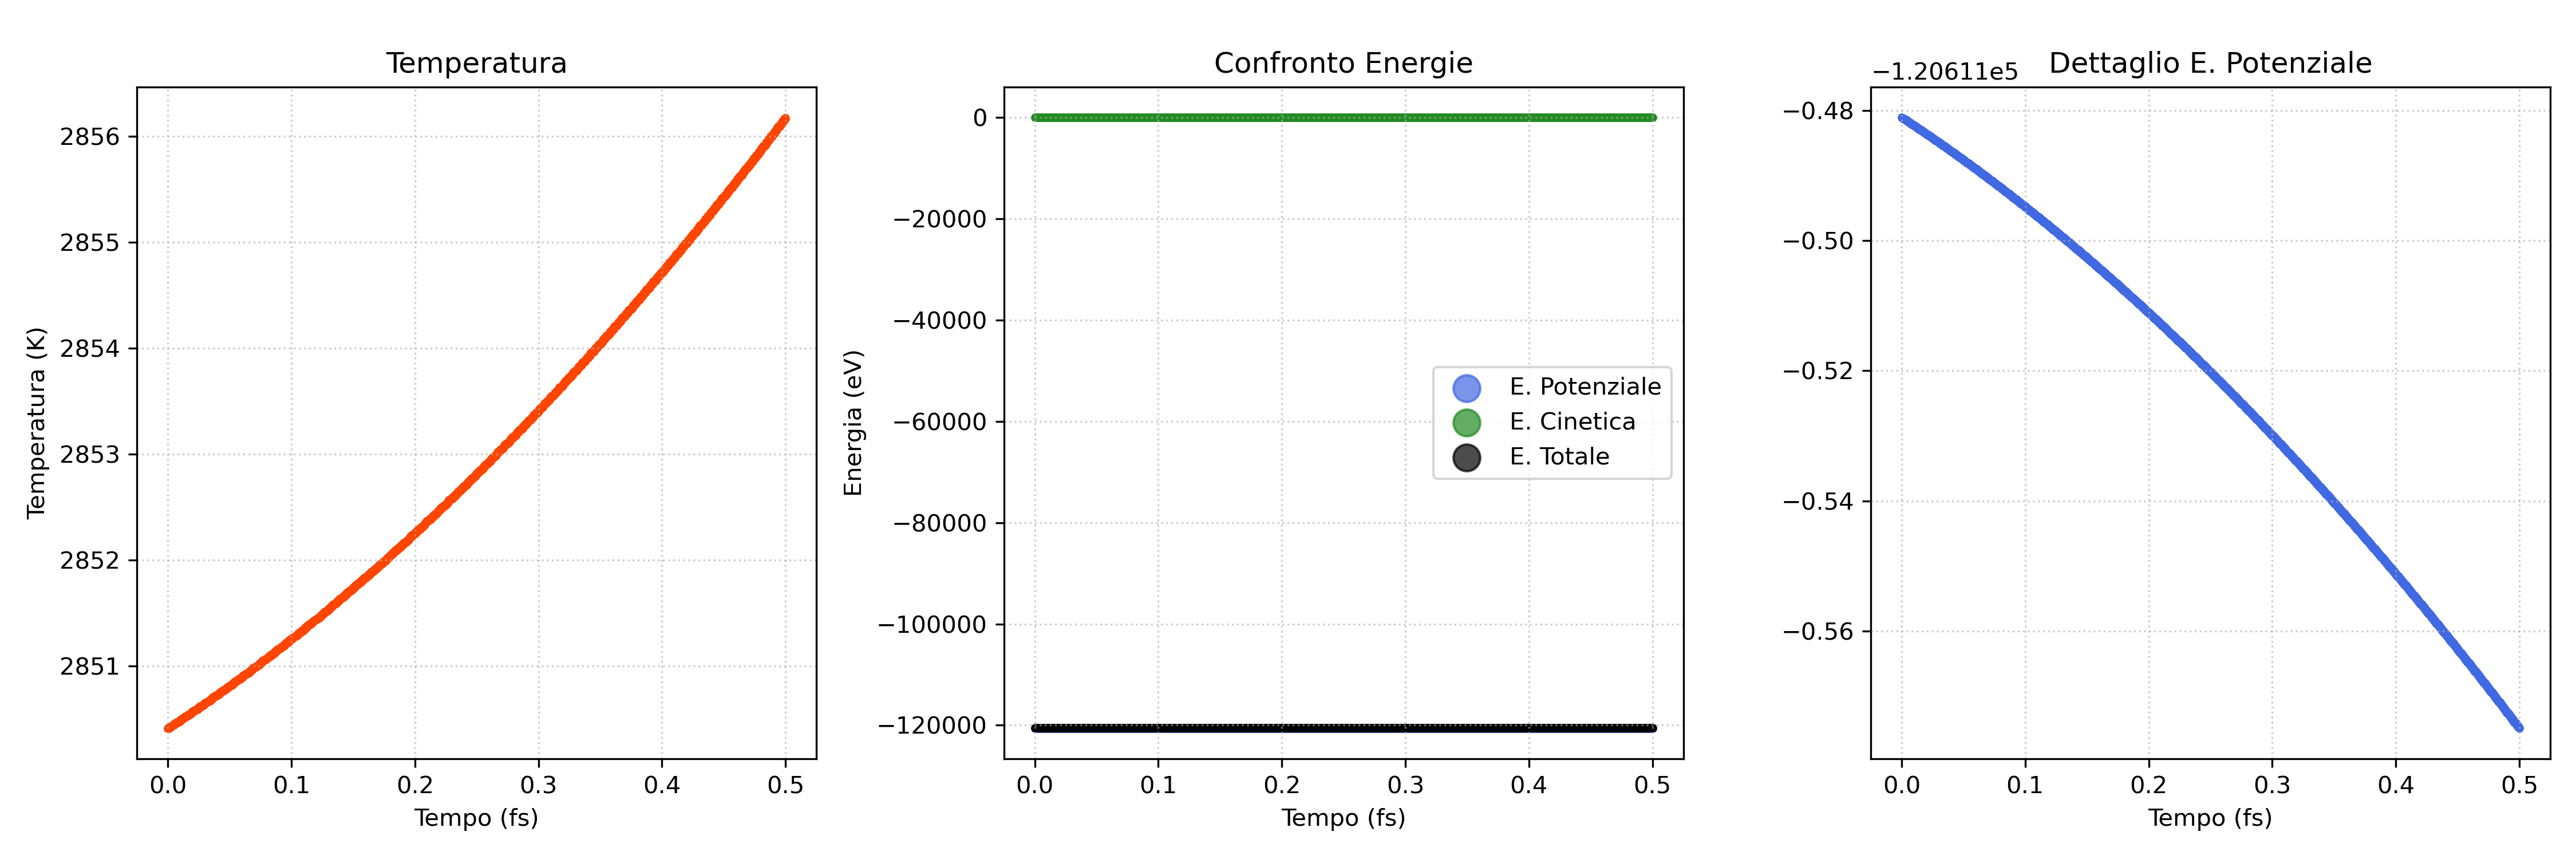
\includegraphics[scale=0.40]{./img/andamento_energia_nve_timestep.png}
    \caption{Grafico dell'andamento temporale per i valori di energia e temperatura}
    \label{fig:andamento_nve_energie_timestep}
\end{figure}


\begin{figure}[h]
    \centering
    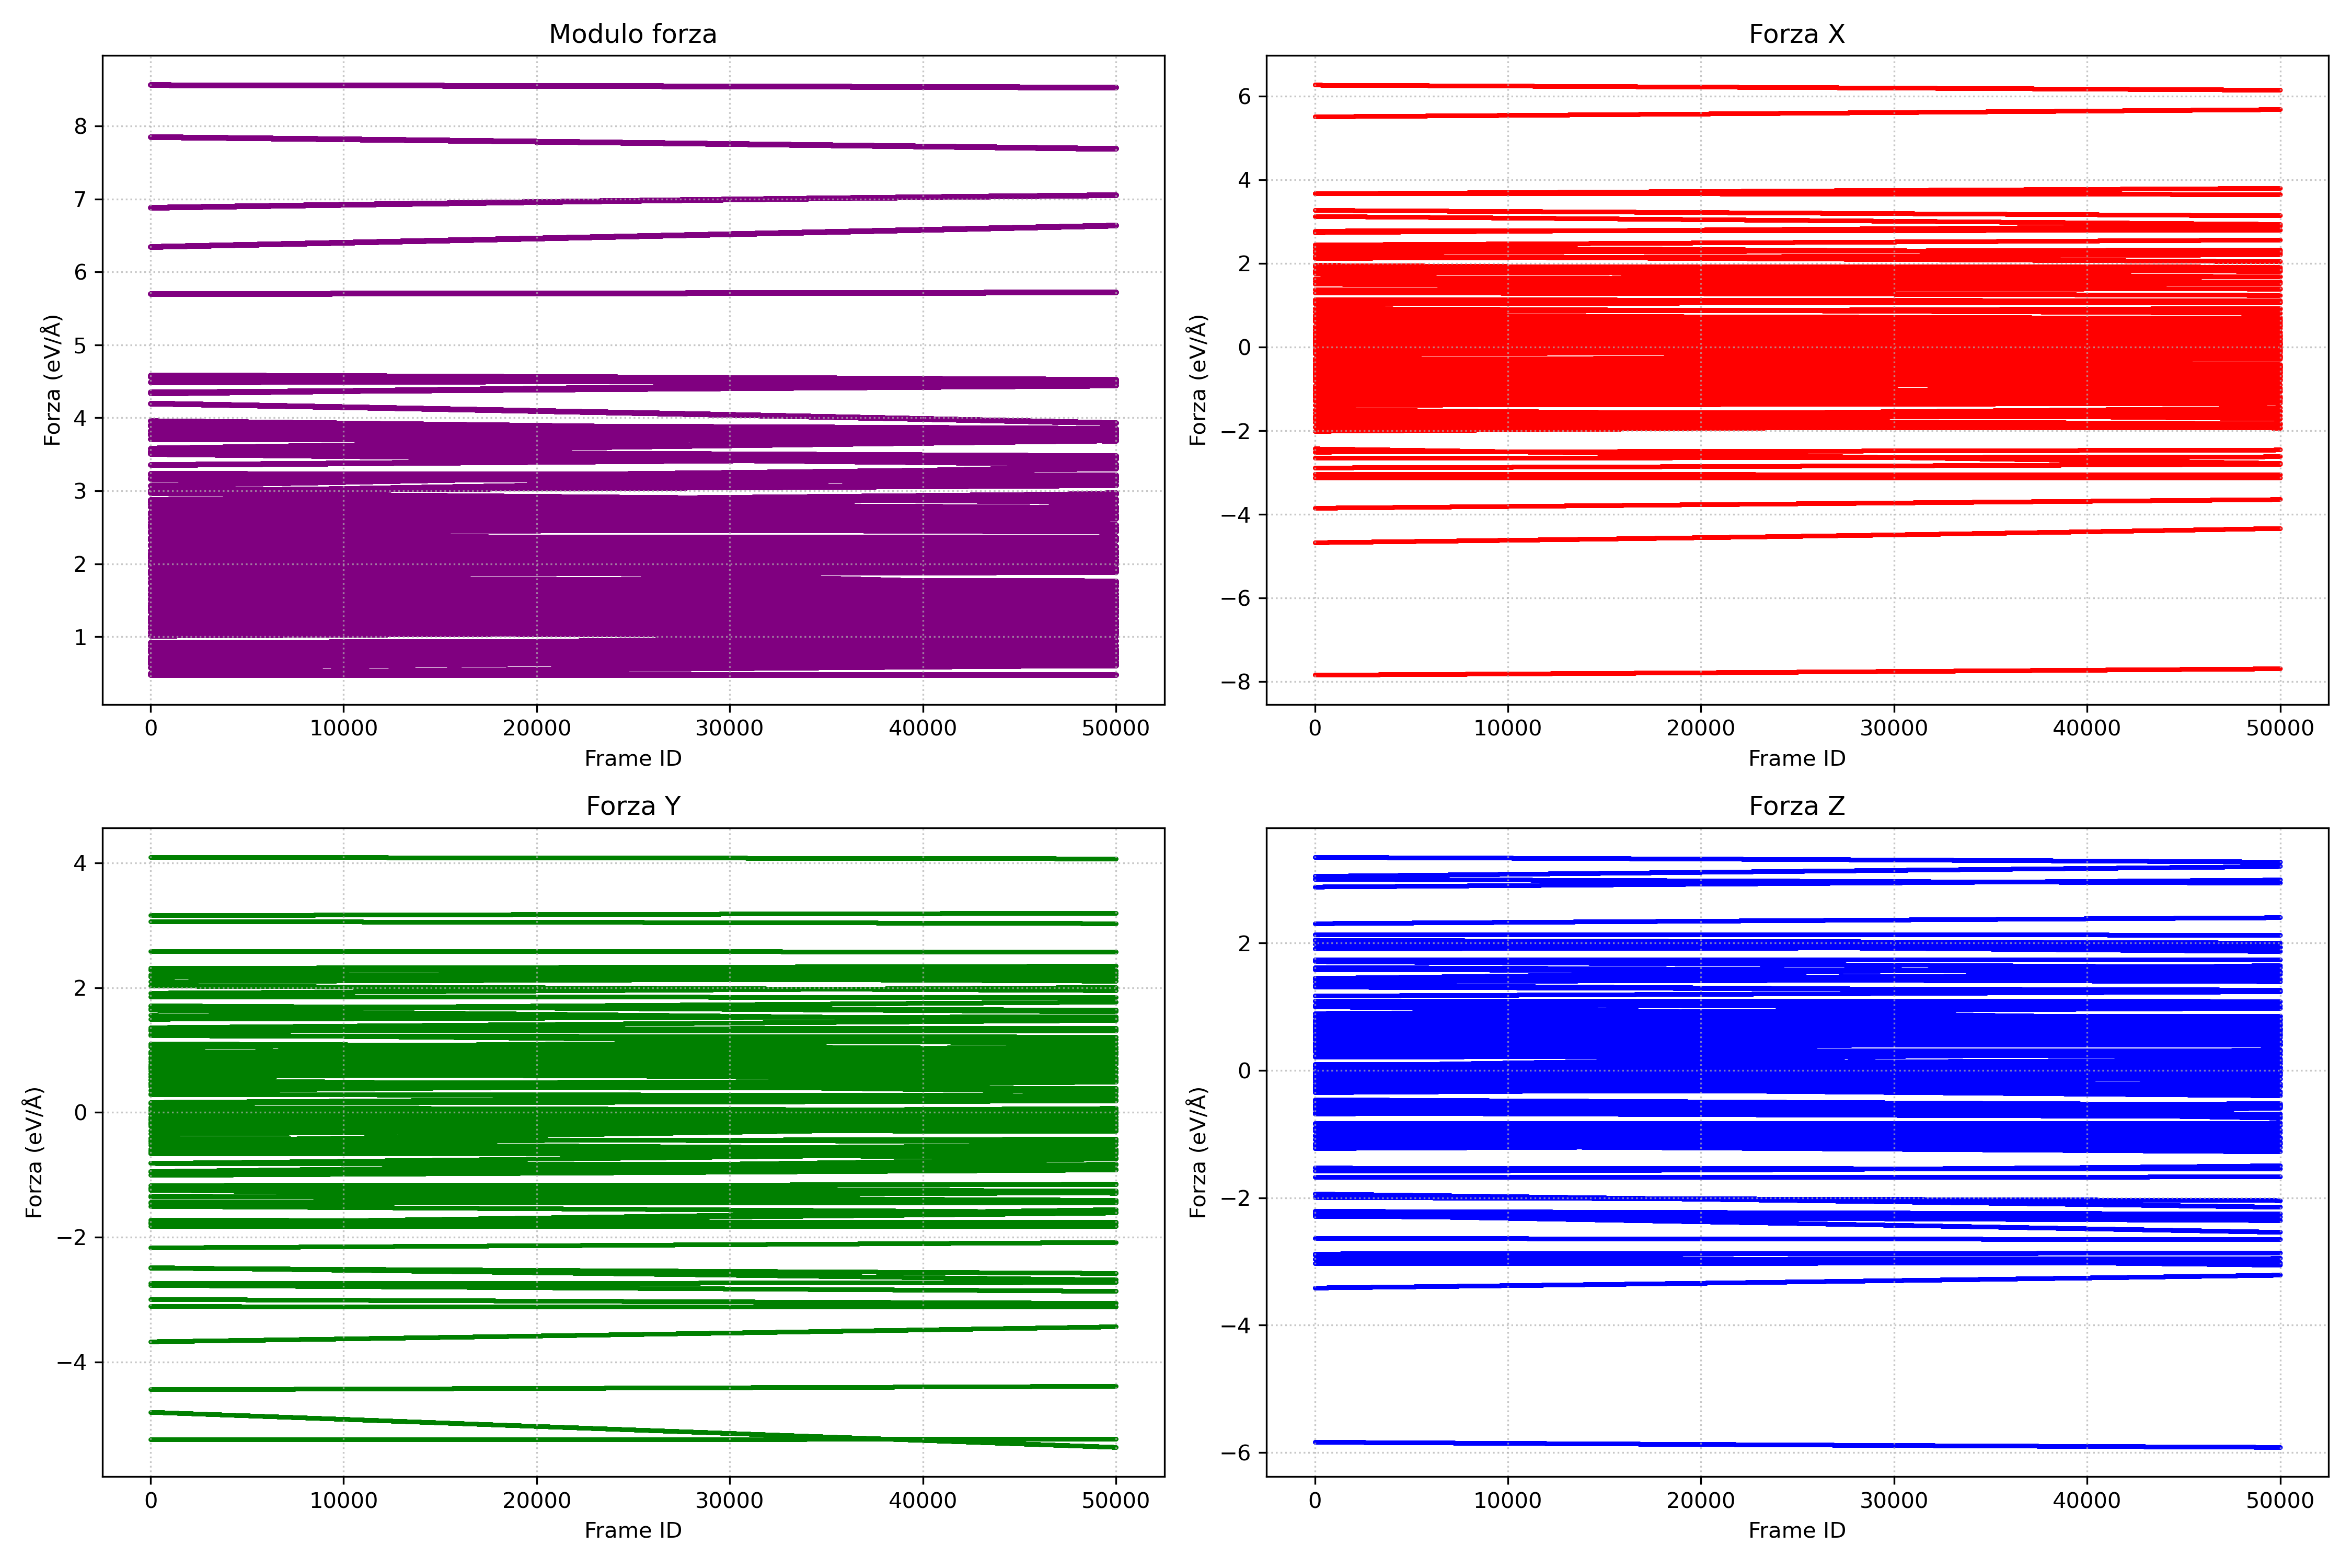
\includegraphics[scale=0.40]{./img/andamento_forze_totali_blocchi_nve_timestep.png}
    \caption{Grafico dell'andamento temporale per i valori di forza, sia in modulo che divise per componenti.}
    \label{fig:andamento_nve_forze_timestep}
\end{figure}


Considerando questo risultato (\autoref{fig:andamento_nve_energie_timestep}) la prima cosa che si vede è una diminuzione del range in cui i valori di temperatura e di energia variano.
A ogni modo possiamo notare che entrambe mantengono la medesima forma vista in precedenza, possiamo quindi presumere che stiano comunque divergendo, ma a un rate estremamente basso.
Anche i valori delle forze sono contenuti.
Considerando la tipologia di integratore numerico utilizzato in questa simulazione, questo risultato era prevedibile.


\subsection{Distanze e forze}

Risulta utile andare a guardare la distribuzione dei valori delle distanze tra i primi vicini, per ogni frame si prende come atomo il $j$-esimo e se ne calcola la distanza con i restanti 125, se ne prende poi il minimo, questo per ogni atomo presente nel frame. Successivamente guardiamo la relazione tra i valori di distanza e i valori di forza.
Nel grafico a due pannelli successivo vogliamo evidenziare queste relazioni.
\\

Per il caso del semplice potenziale GAP, come notiamo nella \autoref{fig:confronto_forze_distanze_gap_testdata}, la maggior parte dei valori di distanza si trova al di sotto del valore di $1.5$ \AA. Si vede facilmente dove le forze assumono il loro valore maggiore.

{
\begin{figure}[ht]
    \centering

    \begin{subfigure}{0.48\textwidth}
        \centering
        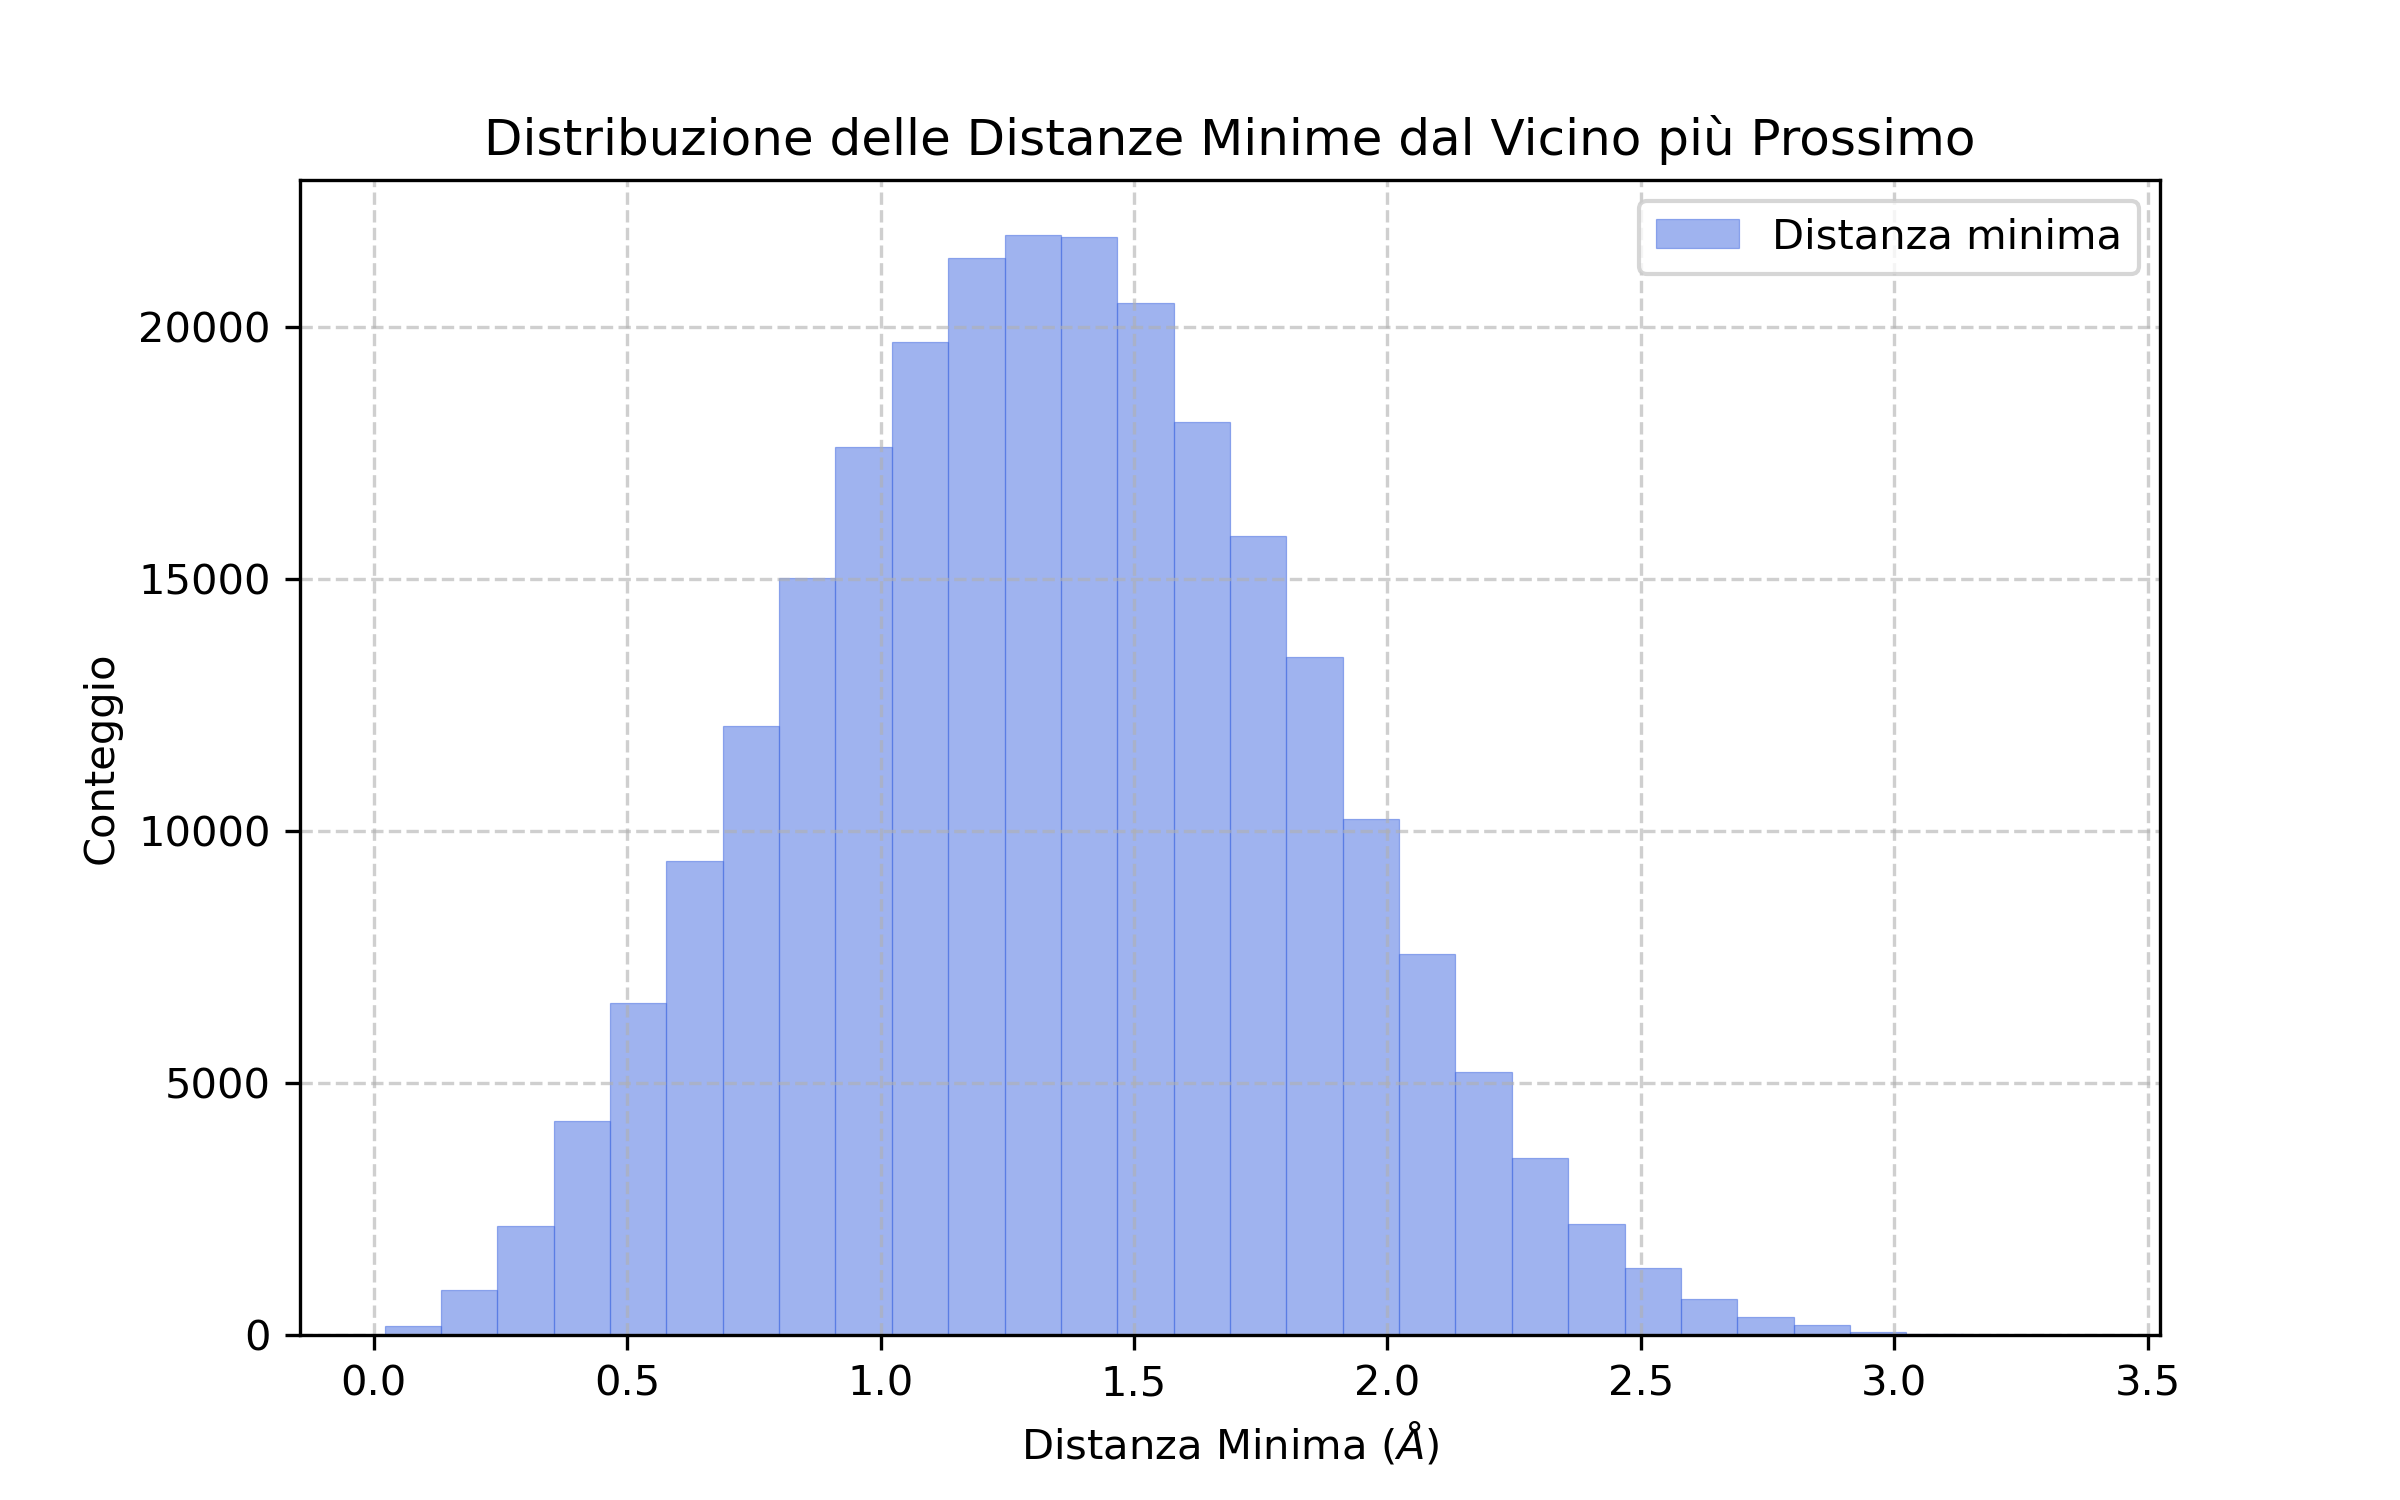
\includegraphics[scale=0.45]{./img/histo_distanze_nve_testdata.png}
        \caption{Istogramma dei valori di distanza tra i primi vicini per il solo potenziale GAP}
    \end{subfigure}
    \hfill
    \begin{subfigure}{0.48\textwidth}
        \centering
        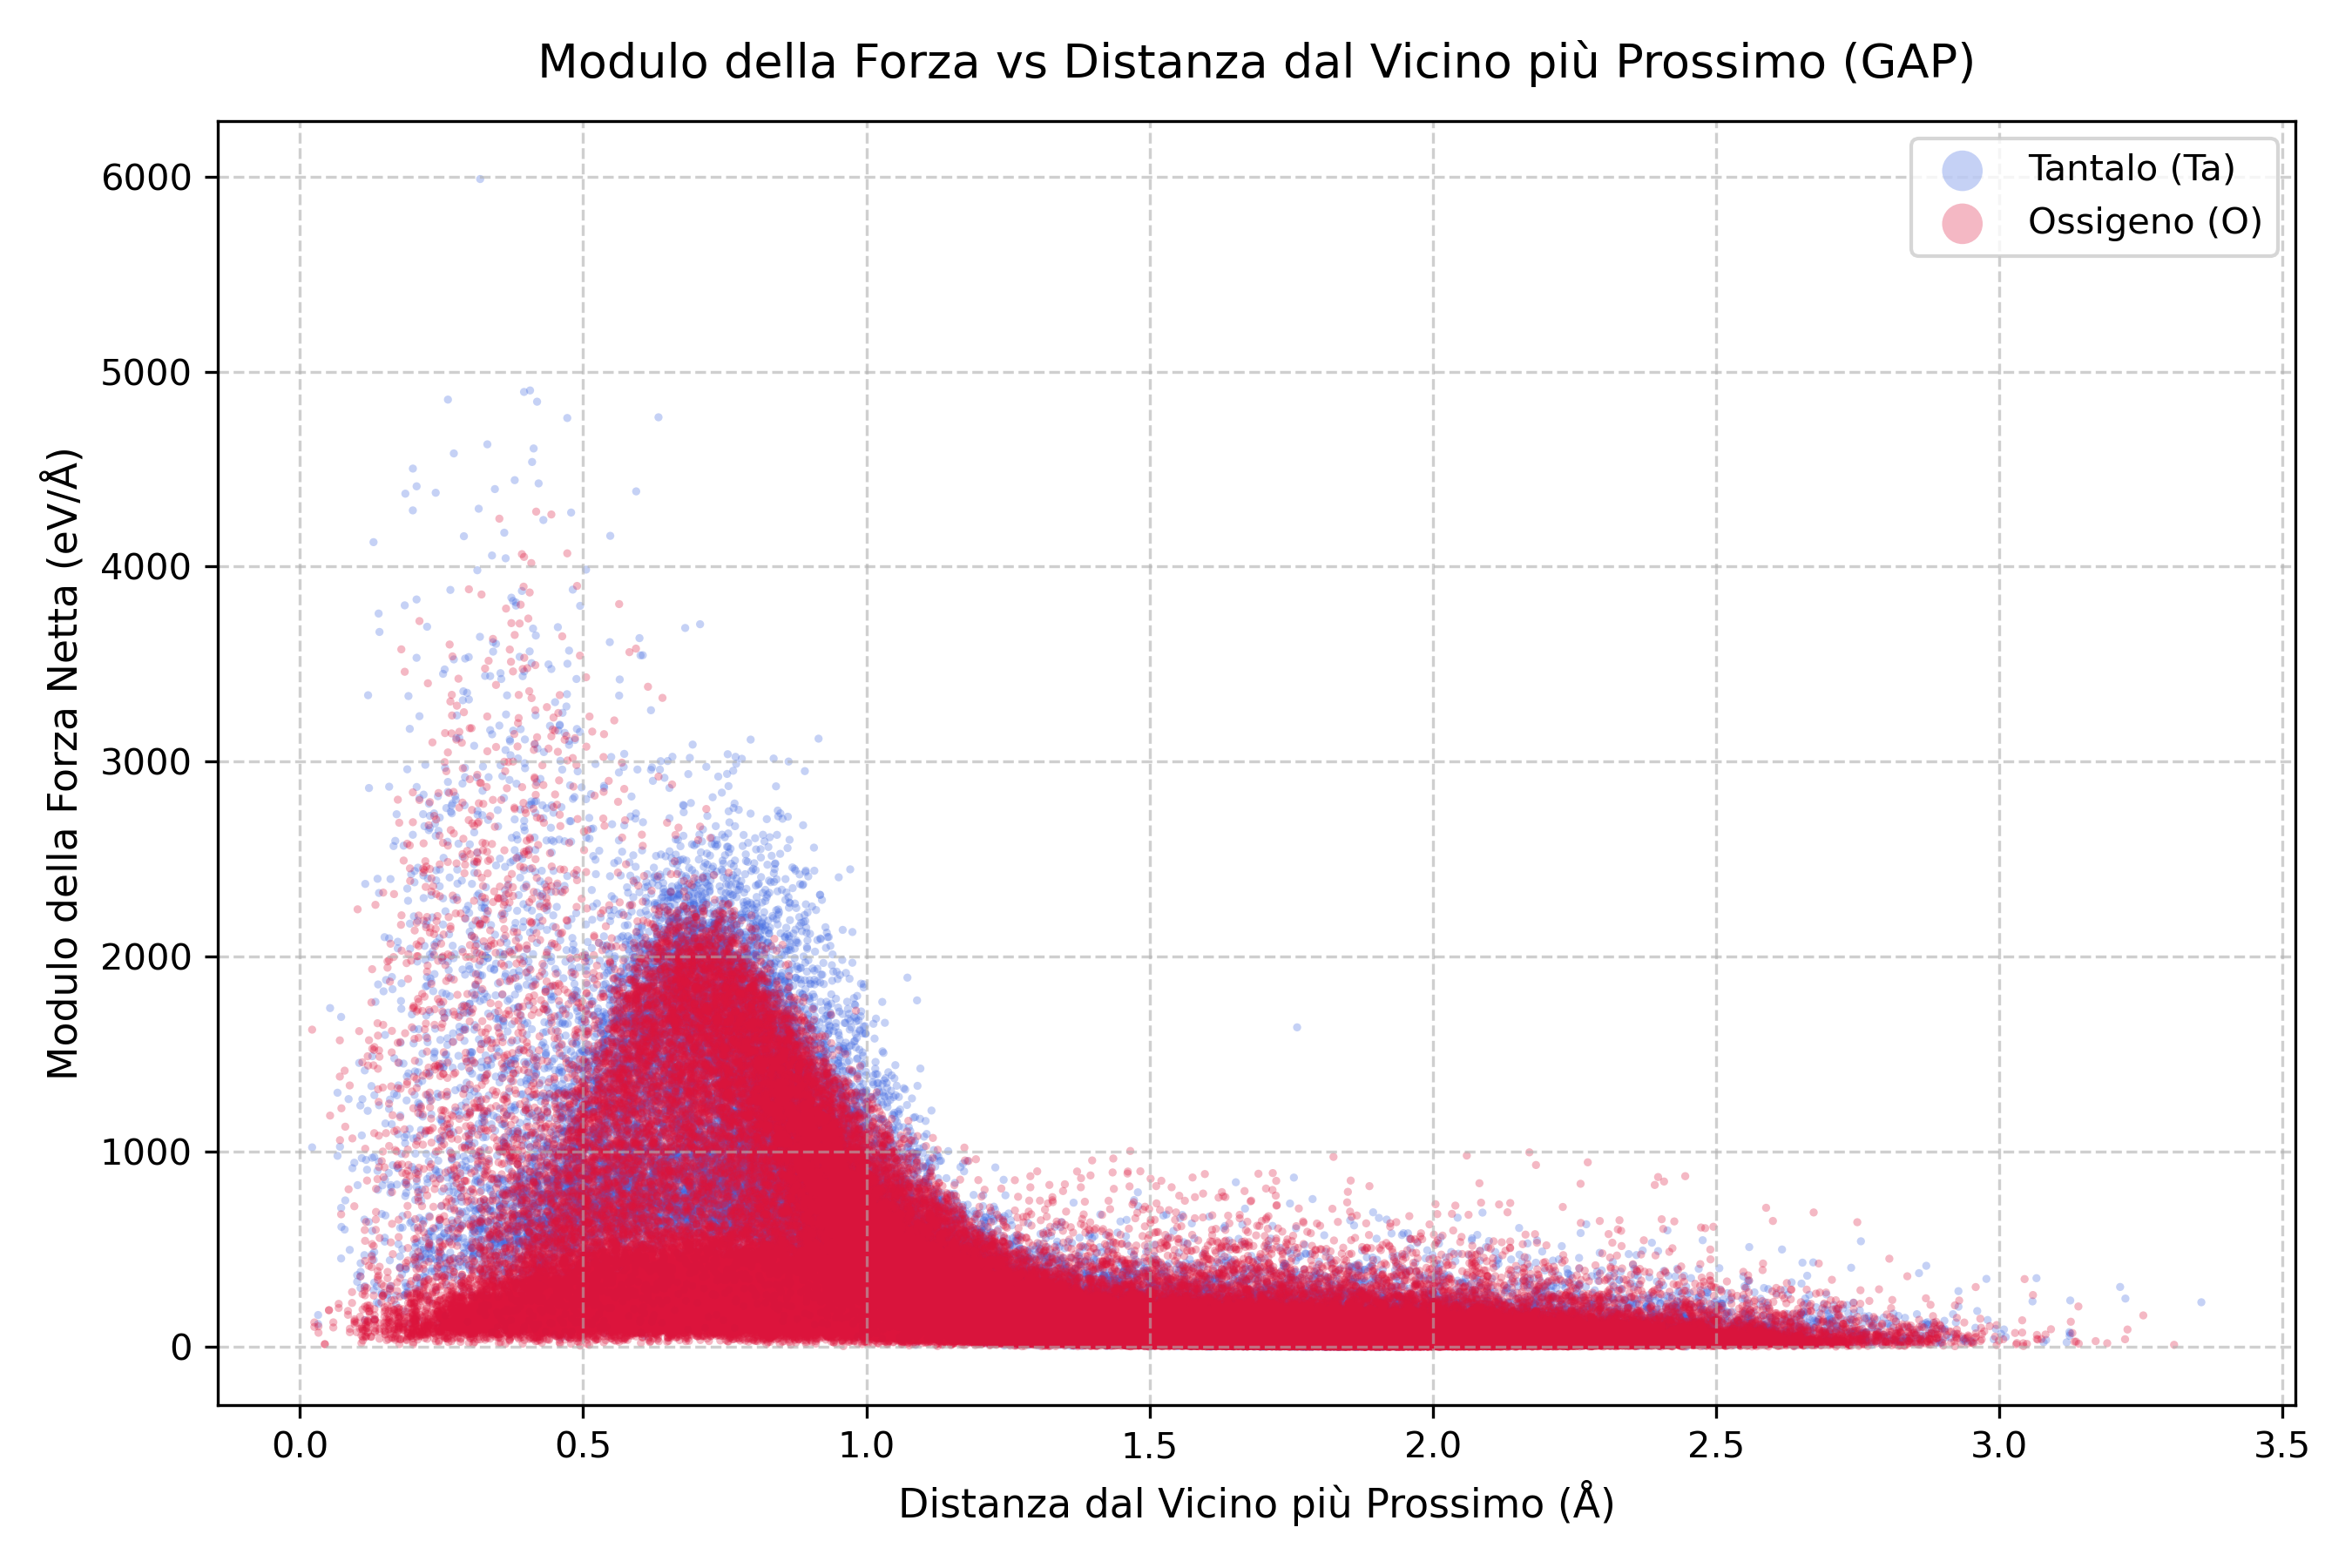
\includegraphics[scale=0.37]{./img/andamento_forze_totali_distanza_nve_testdata.png}
        \caption{Relazione tra i valori di forza e distanza tra i primi vicini}
    \end{subfigure}

    \caption{Distanze e relazione forze-distanze per il caso del solo potenziale GAP}
    \label{fig:confronto_forze_distanze_gap_testdata}
\end{figure}
}

Questo diventa rilevante nel momento in cui andiamo ad analizzare i valori di distanza tra i primi vicini e le relative forze, calcolati nel medesimo modo, presenti nelle configurazioni utilizzate nella fase di training, queste sono riportate in \autoref{fig:confronto_forze_distanze_qe_traindata}, quello che notiamo immediatamente, dopo la limitatezza dei valori delle forze, è come la distanza tra i primi vicini assume valori tutti superiori agli $1.5$\AA, inoltre vediamo, che come ci si aspetterebbe, i valori delle forze aumentano alla diminuzione della distanza.

{
\begin{figure}[ht]
    \centering

    \begin{subfigure}{0.48\textwidth}
        \centering
        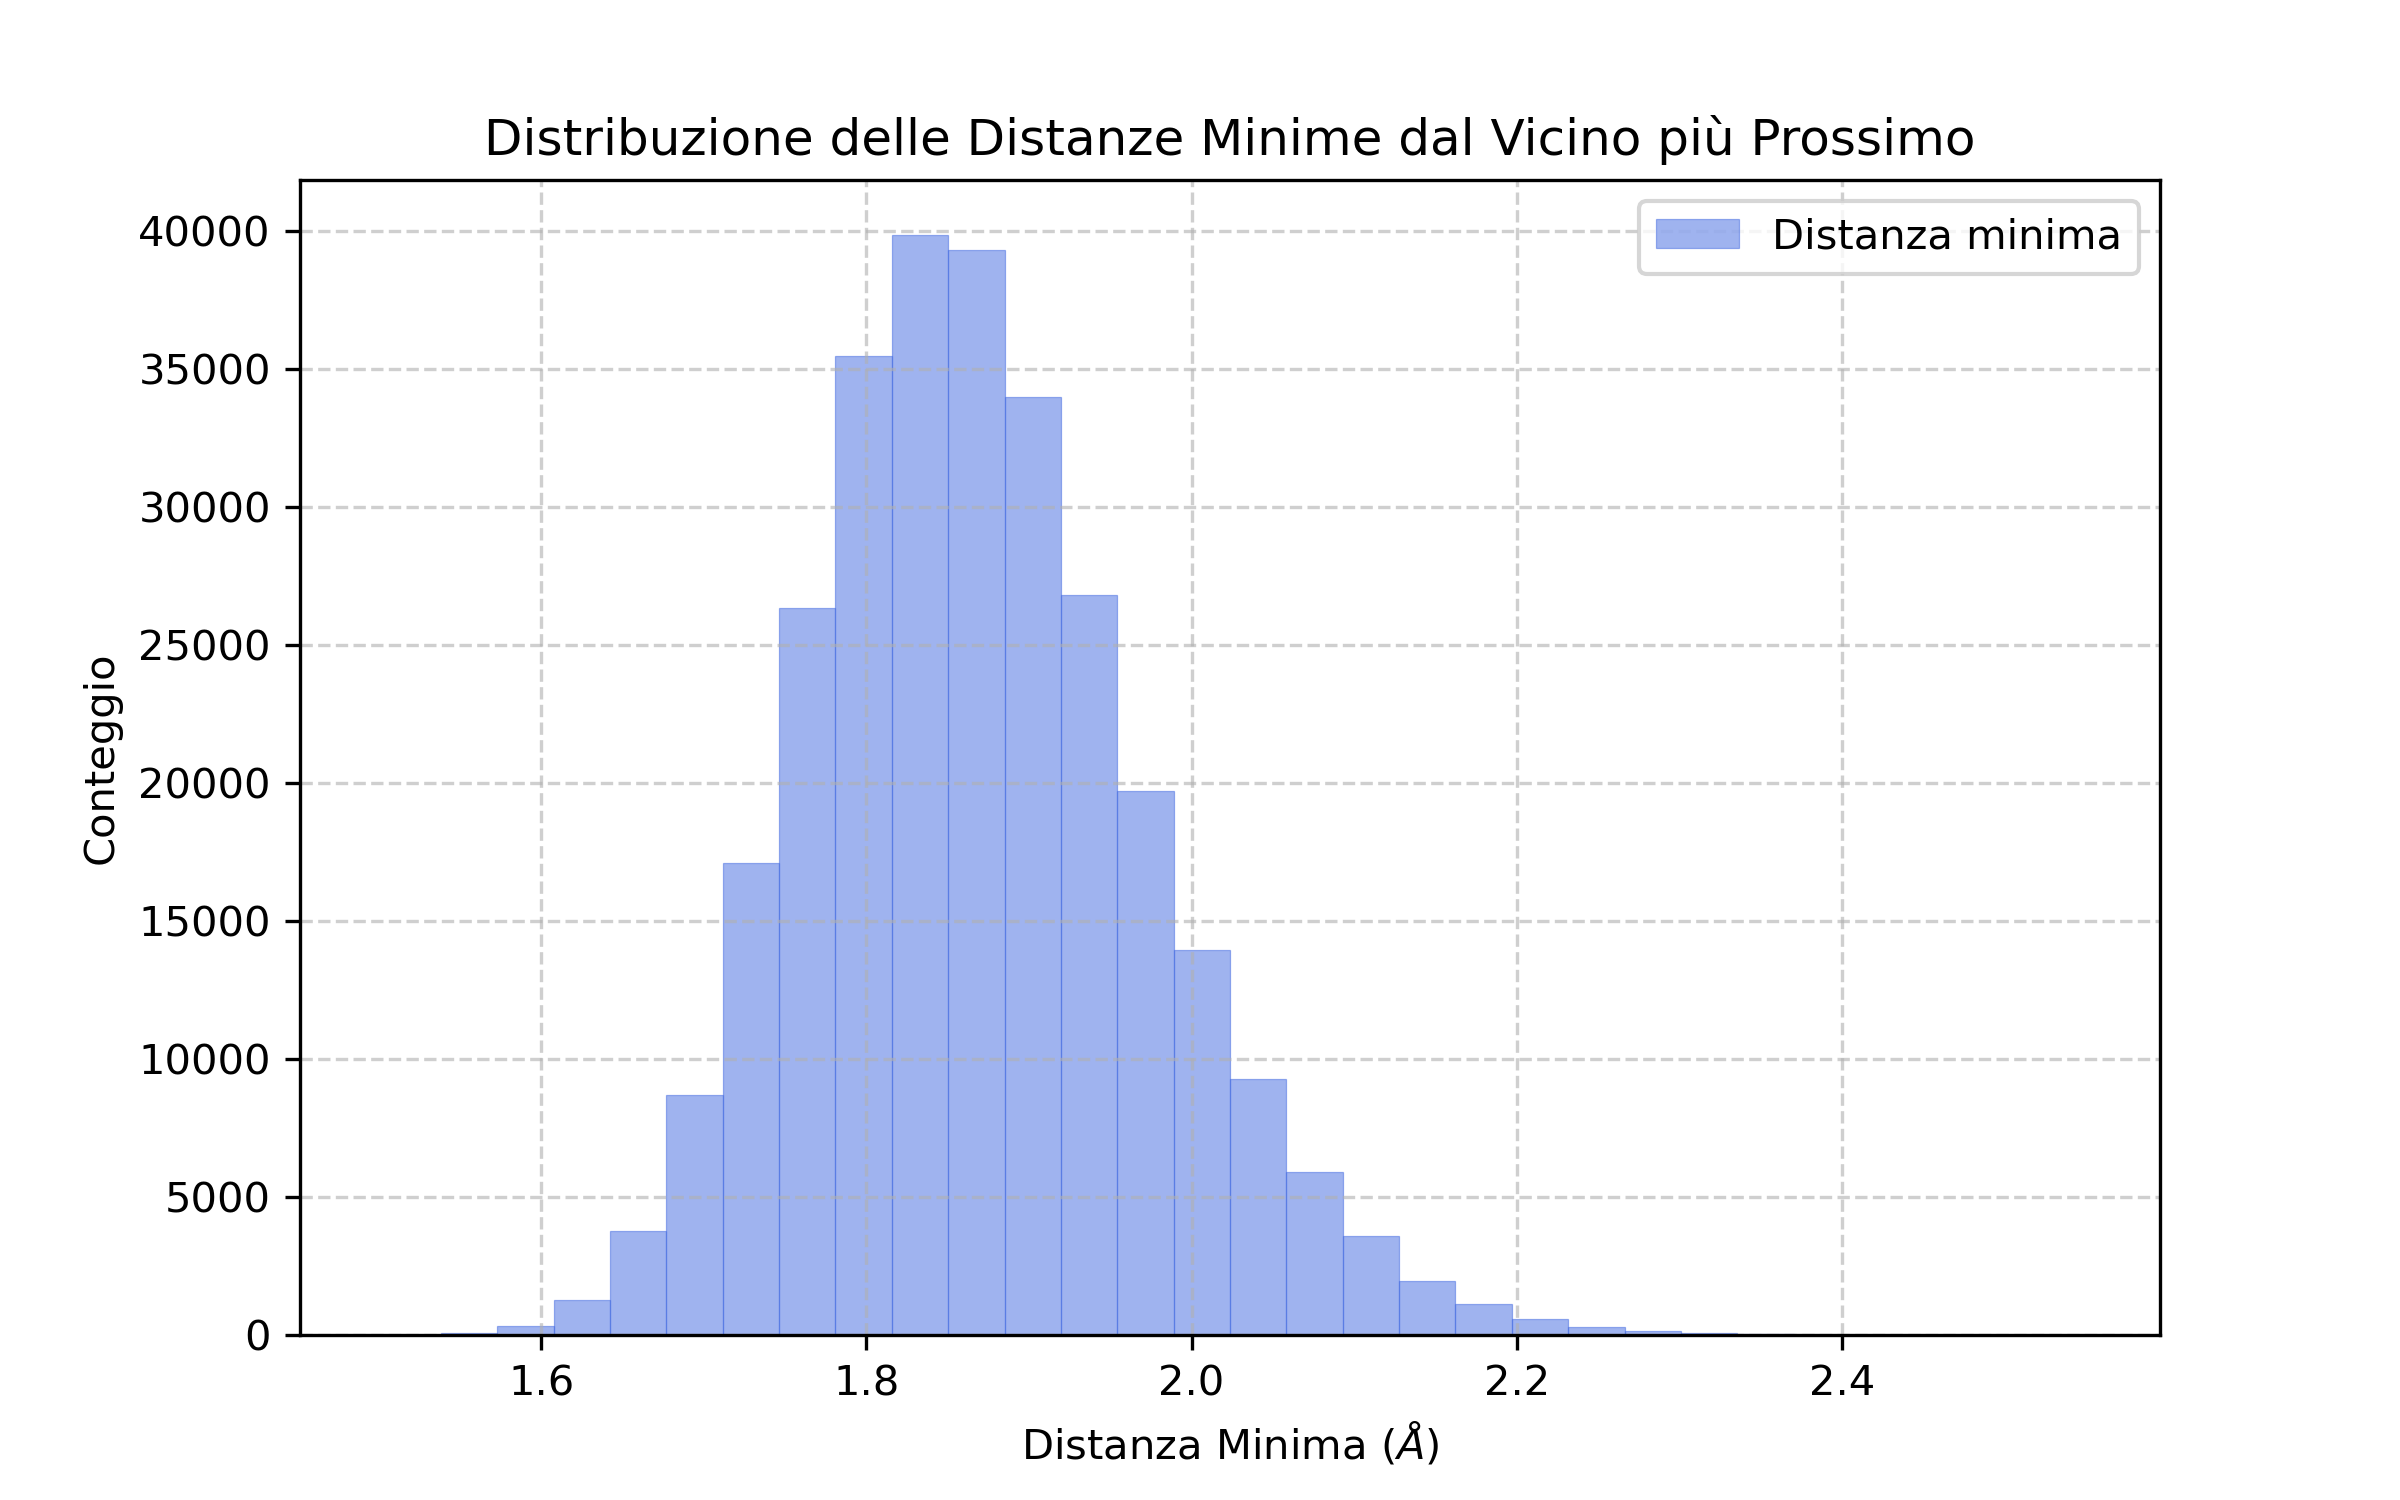
\includegraphics[scale=0.45]{./img/histo_distanze_qe_traindata.png}
        \caption{Istogramma dei valori di distanza tra i primi vicini per il set di dati di training}
    \end{subfigure}
    \hfill
    \begin{subfigure}{0.48\textwidth}
        \centering
        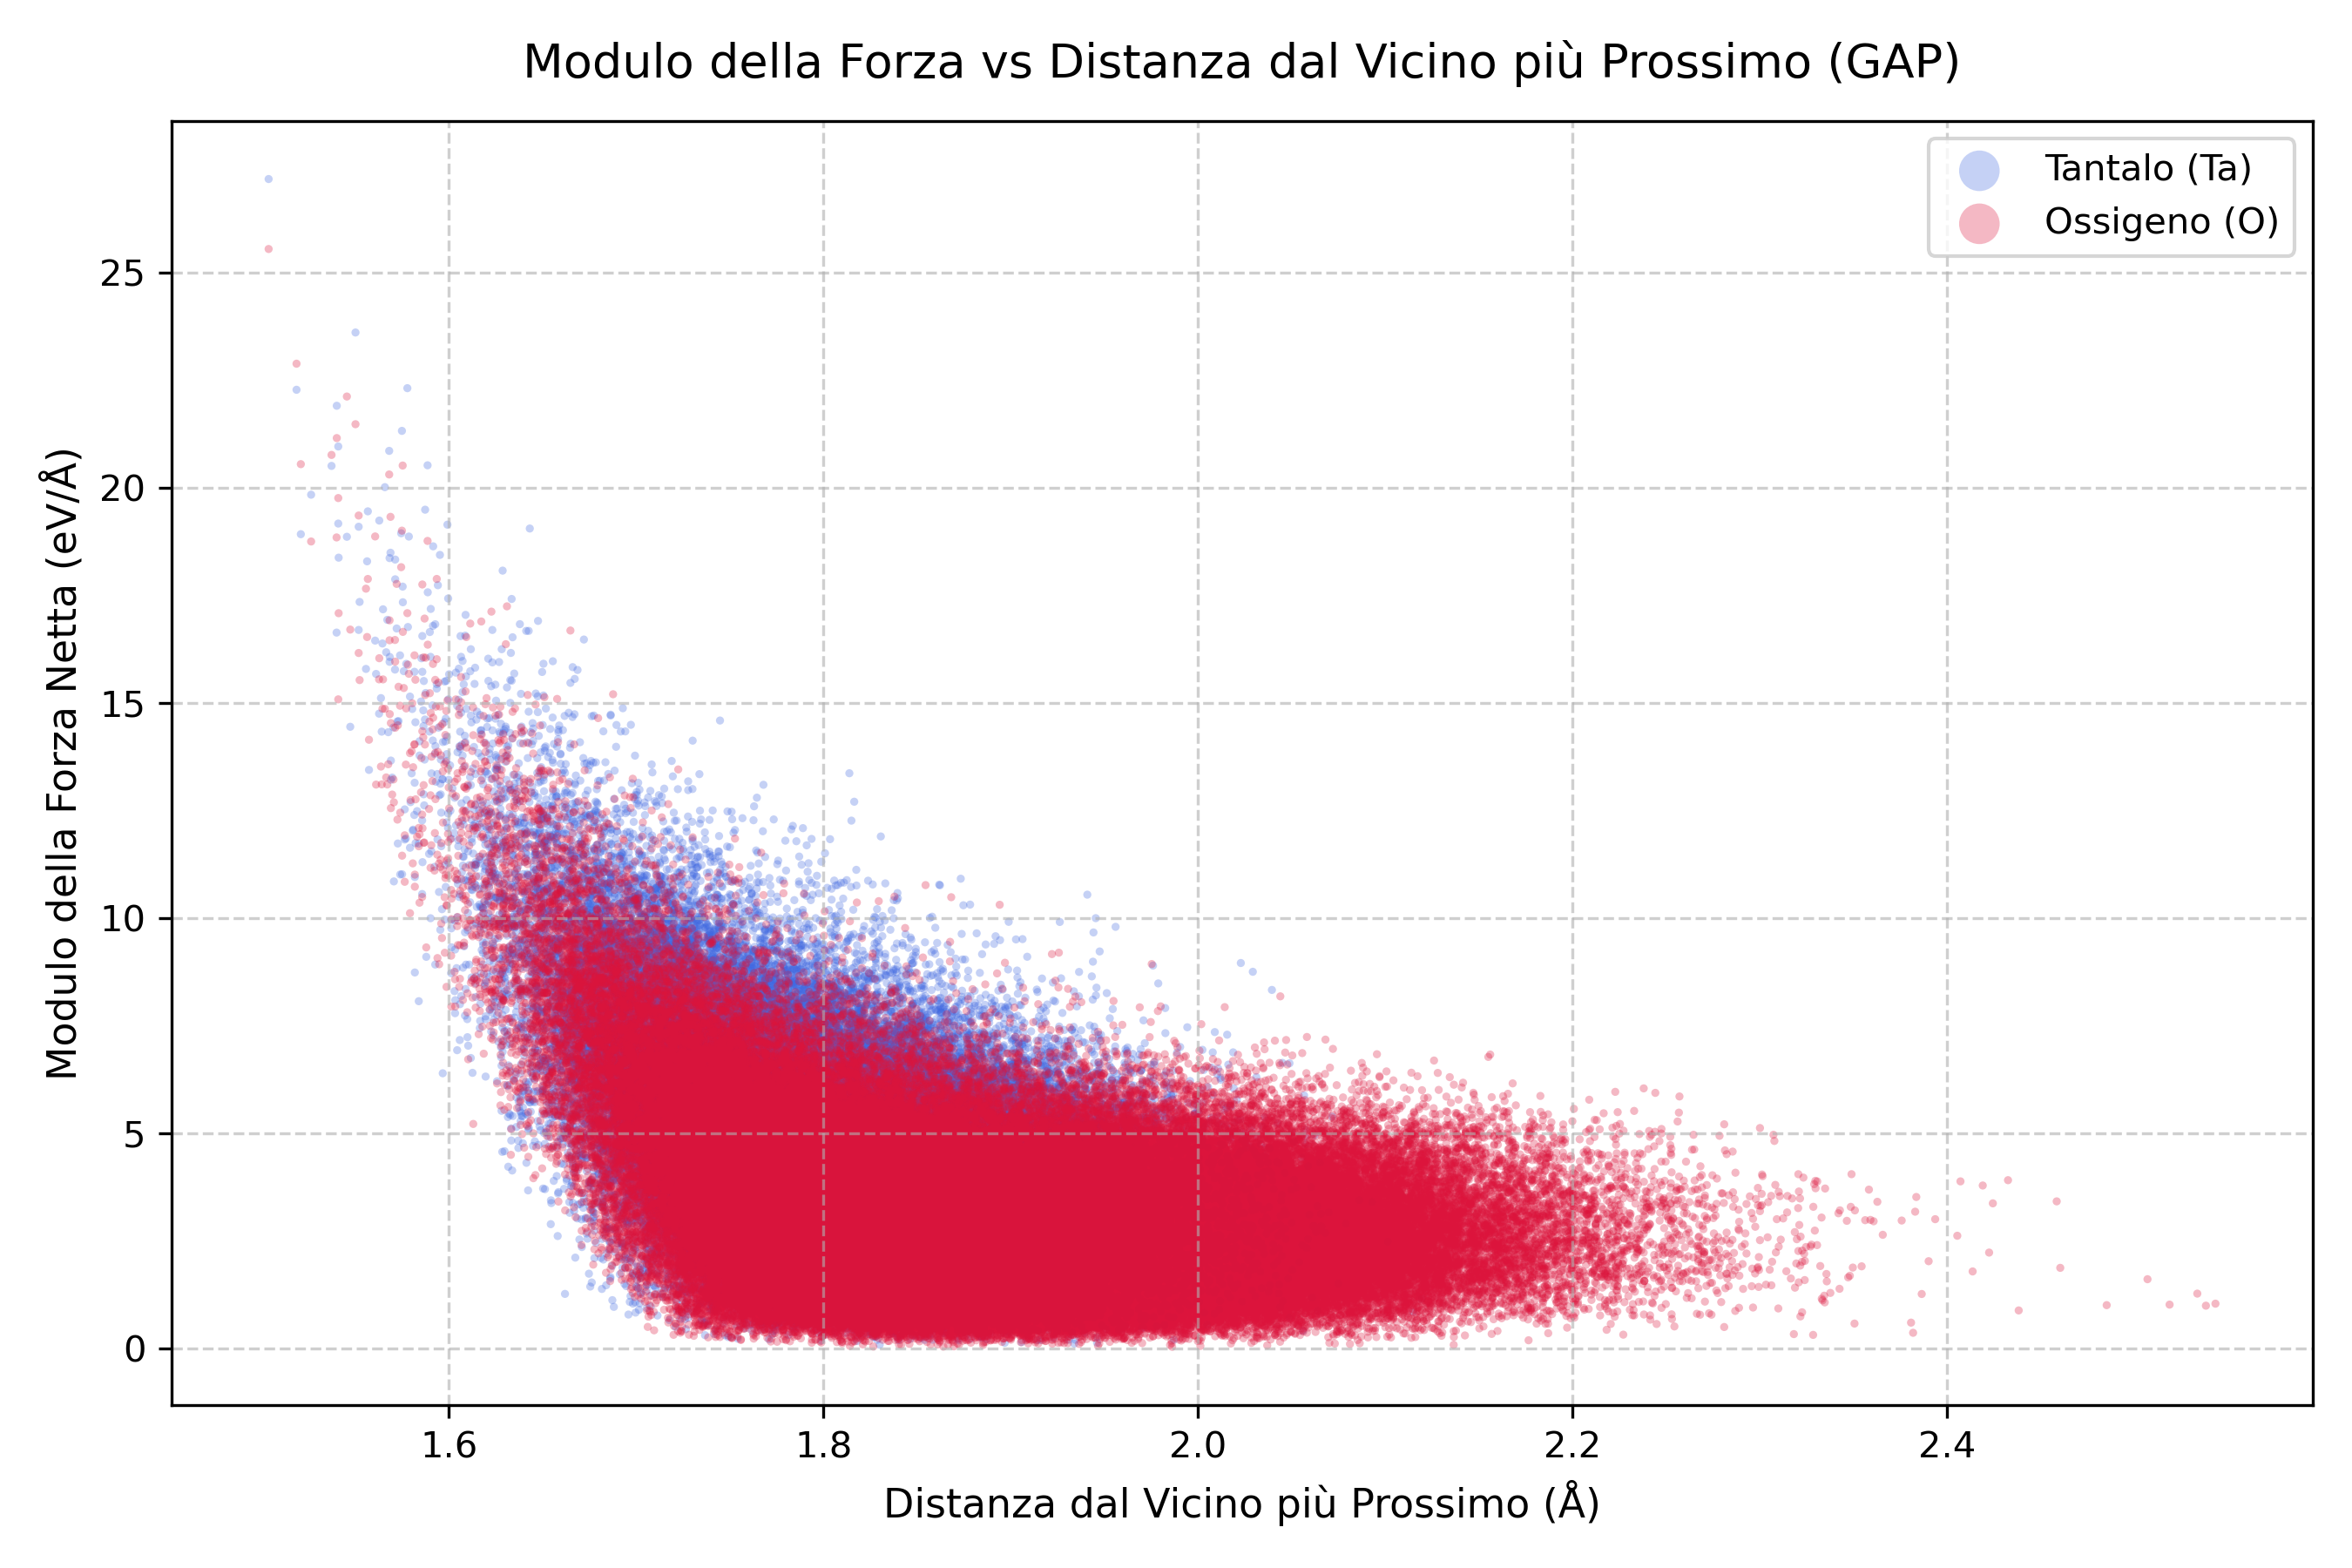
\includegraphics[scale=0.37]{./img/andamento_forze_totali_distanza_qe_traindata.png}
        \caption{Relazione tra i valori di forza e distanza tra i primi vicini per il set di dati di training}
    \end{subfigure}

    \caption{Distanze e relazione forze-distanze per il set di dati di training prodotto con QE.}
    \label{fig:confronto_forze_distanze_qe_traindata}
\end{figure}
}


\section{Simulazione con ZBL}

I risultati della sezione precedente sono il principale motivo per il quale andiamo ad addizionare un potenziale repulsivo come lo ZBL.

Anche in questo caso sono stati svolti diversi test, cambiando di volta in volta diversi parametri, non riteniamo necessario riportare tutti questi risultati, inseriamo solo uno di questi, dove l'unica modifica rispetto ai casi precedenti è un timestep di $1$ fs.

I parametri per i raggi che abbiamo utilizzato sono dati dal seguente ragionamento, per il $r_{outer} = 1.5$ \AA \hspace{2pt} abbiamo deciso di impostare un valore prossimo ai minimi registrati nelle configurazioni di training, in questo modo volevamo evitare che lo ZBL si sovrapponesse alle previsioni del GAP. Per quanto riguarda il valore di $r_{inner} = 0.5$ \AA \hspace{2pt} abbiamo inserito un valore al quale gli atomi sarebbero sovrapposti e quindi, anche se potrebbe essere alzato, un limite inferiore che dovrebbe essere invalicabile, come si vedrà questo non avviene.

Riportiamo per prima cosa i valori di energia e temperatura (\autoref{fig:andamento_energia_zbl}):

\begin{figure}[h!]
    \centering
    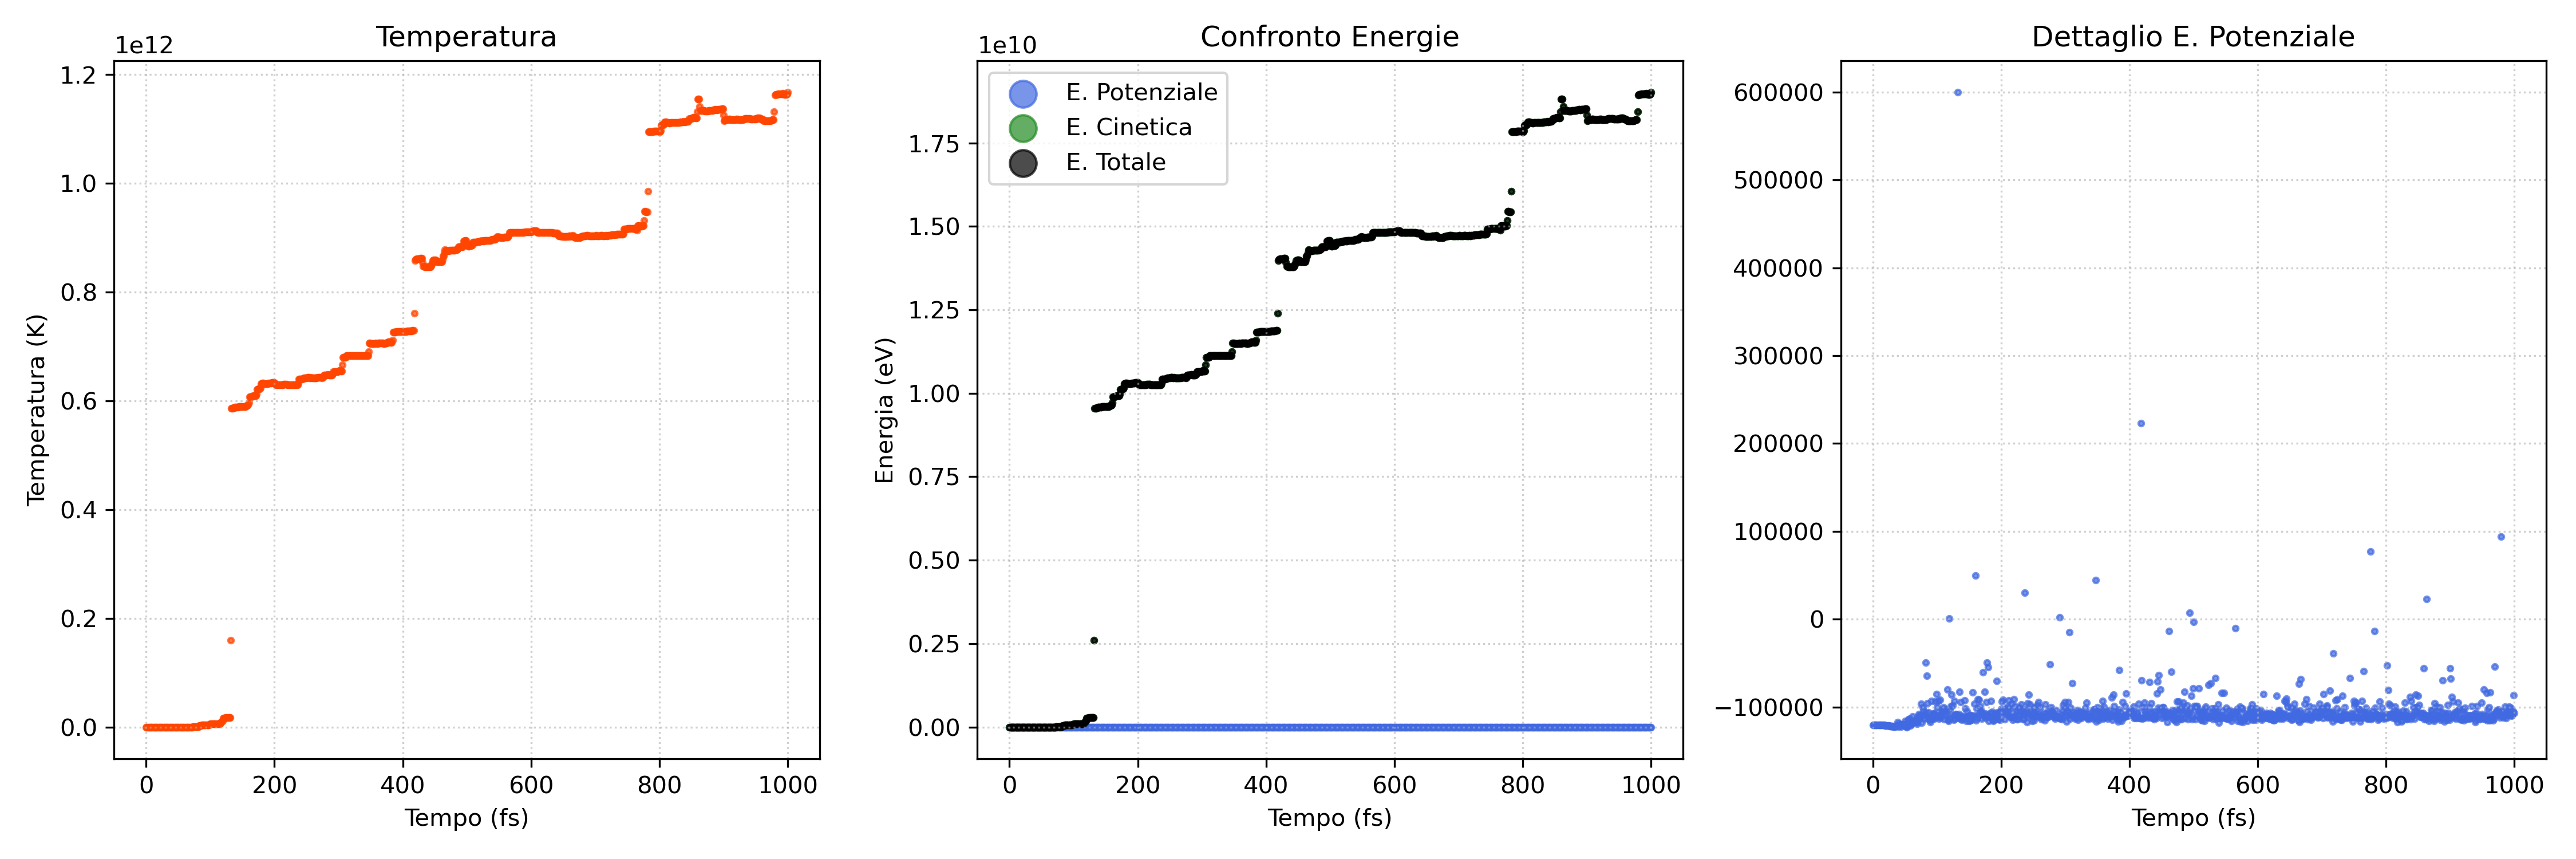
\includegraphics[scale=0.40]{./img/andamento_energia_zbl.png}
    \caption{Grafico dell'andamento temporale per i valori di energia e temperatura, potenziale GAP + ZBL}
    \label{fig:andamento_energia_zbl}
\end{figure}

possiamo vedere come anche in questo caso gli andamenti visti in precedenza si mantengono.

Guardiamo adesso direttamente la relazione tra forze e distanze (\autoref{fig:confronto_forze_distanze_zbl}):

{
\begin{figure}[ht]
    \centering

    \begin{subfigure}{0.48\textwidth}
        \centering
        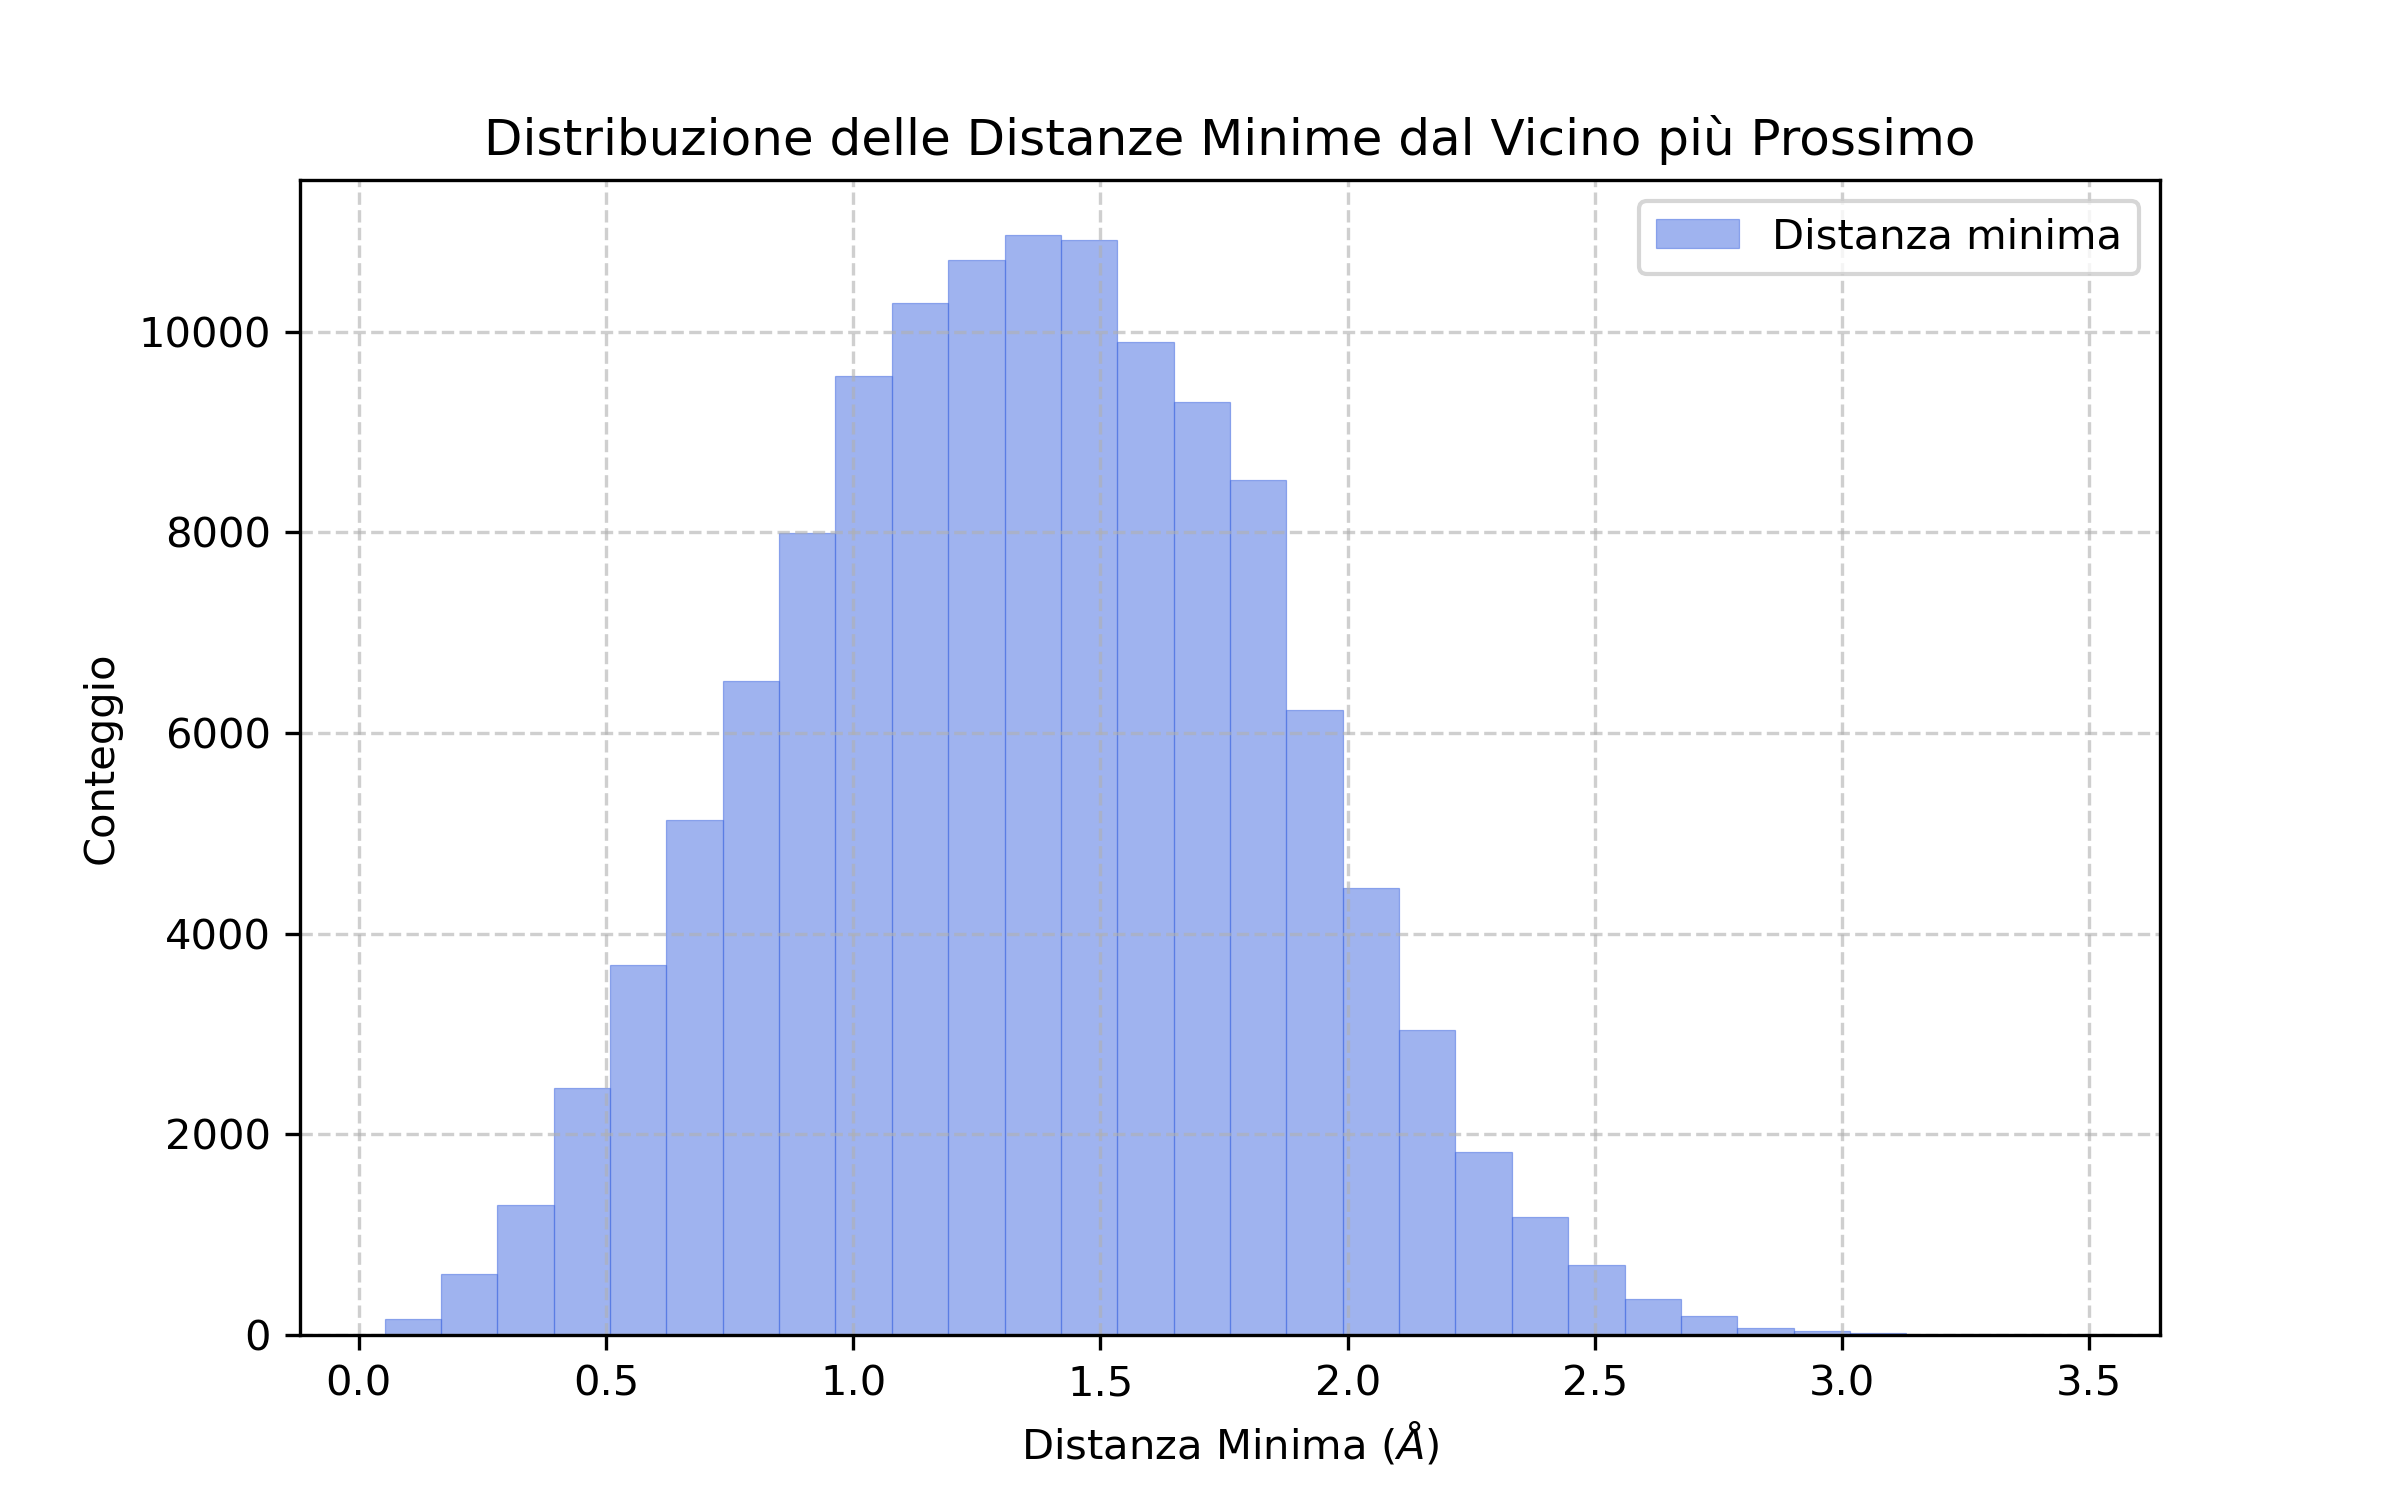
\includegraphics[scale=0.45]{./img/histo_distanze_zbl.png}
        \caption{Istogramma dei valori di distanza tra i primi vicini per il potenziale GAP + ZBL}
    \end{subfigure}
    \hfill
    \begin{subfigure}{0.48\textwidth}
        \centering
        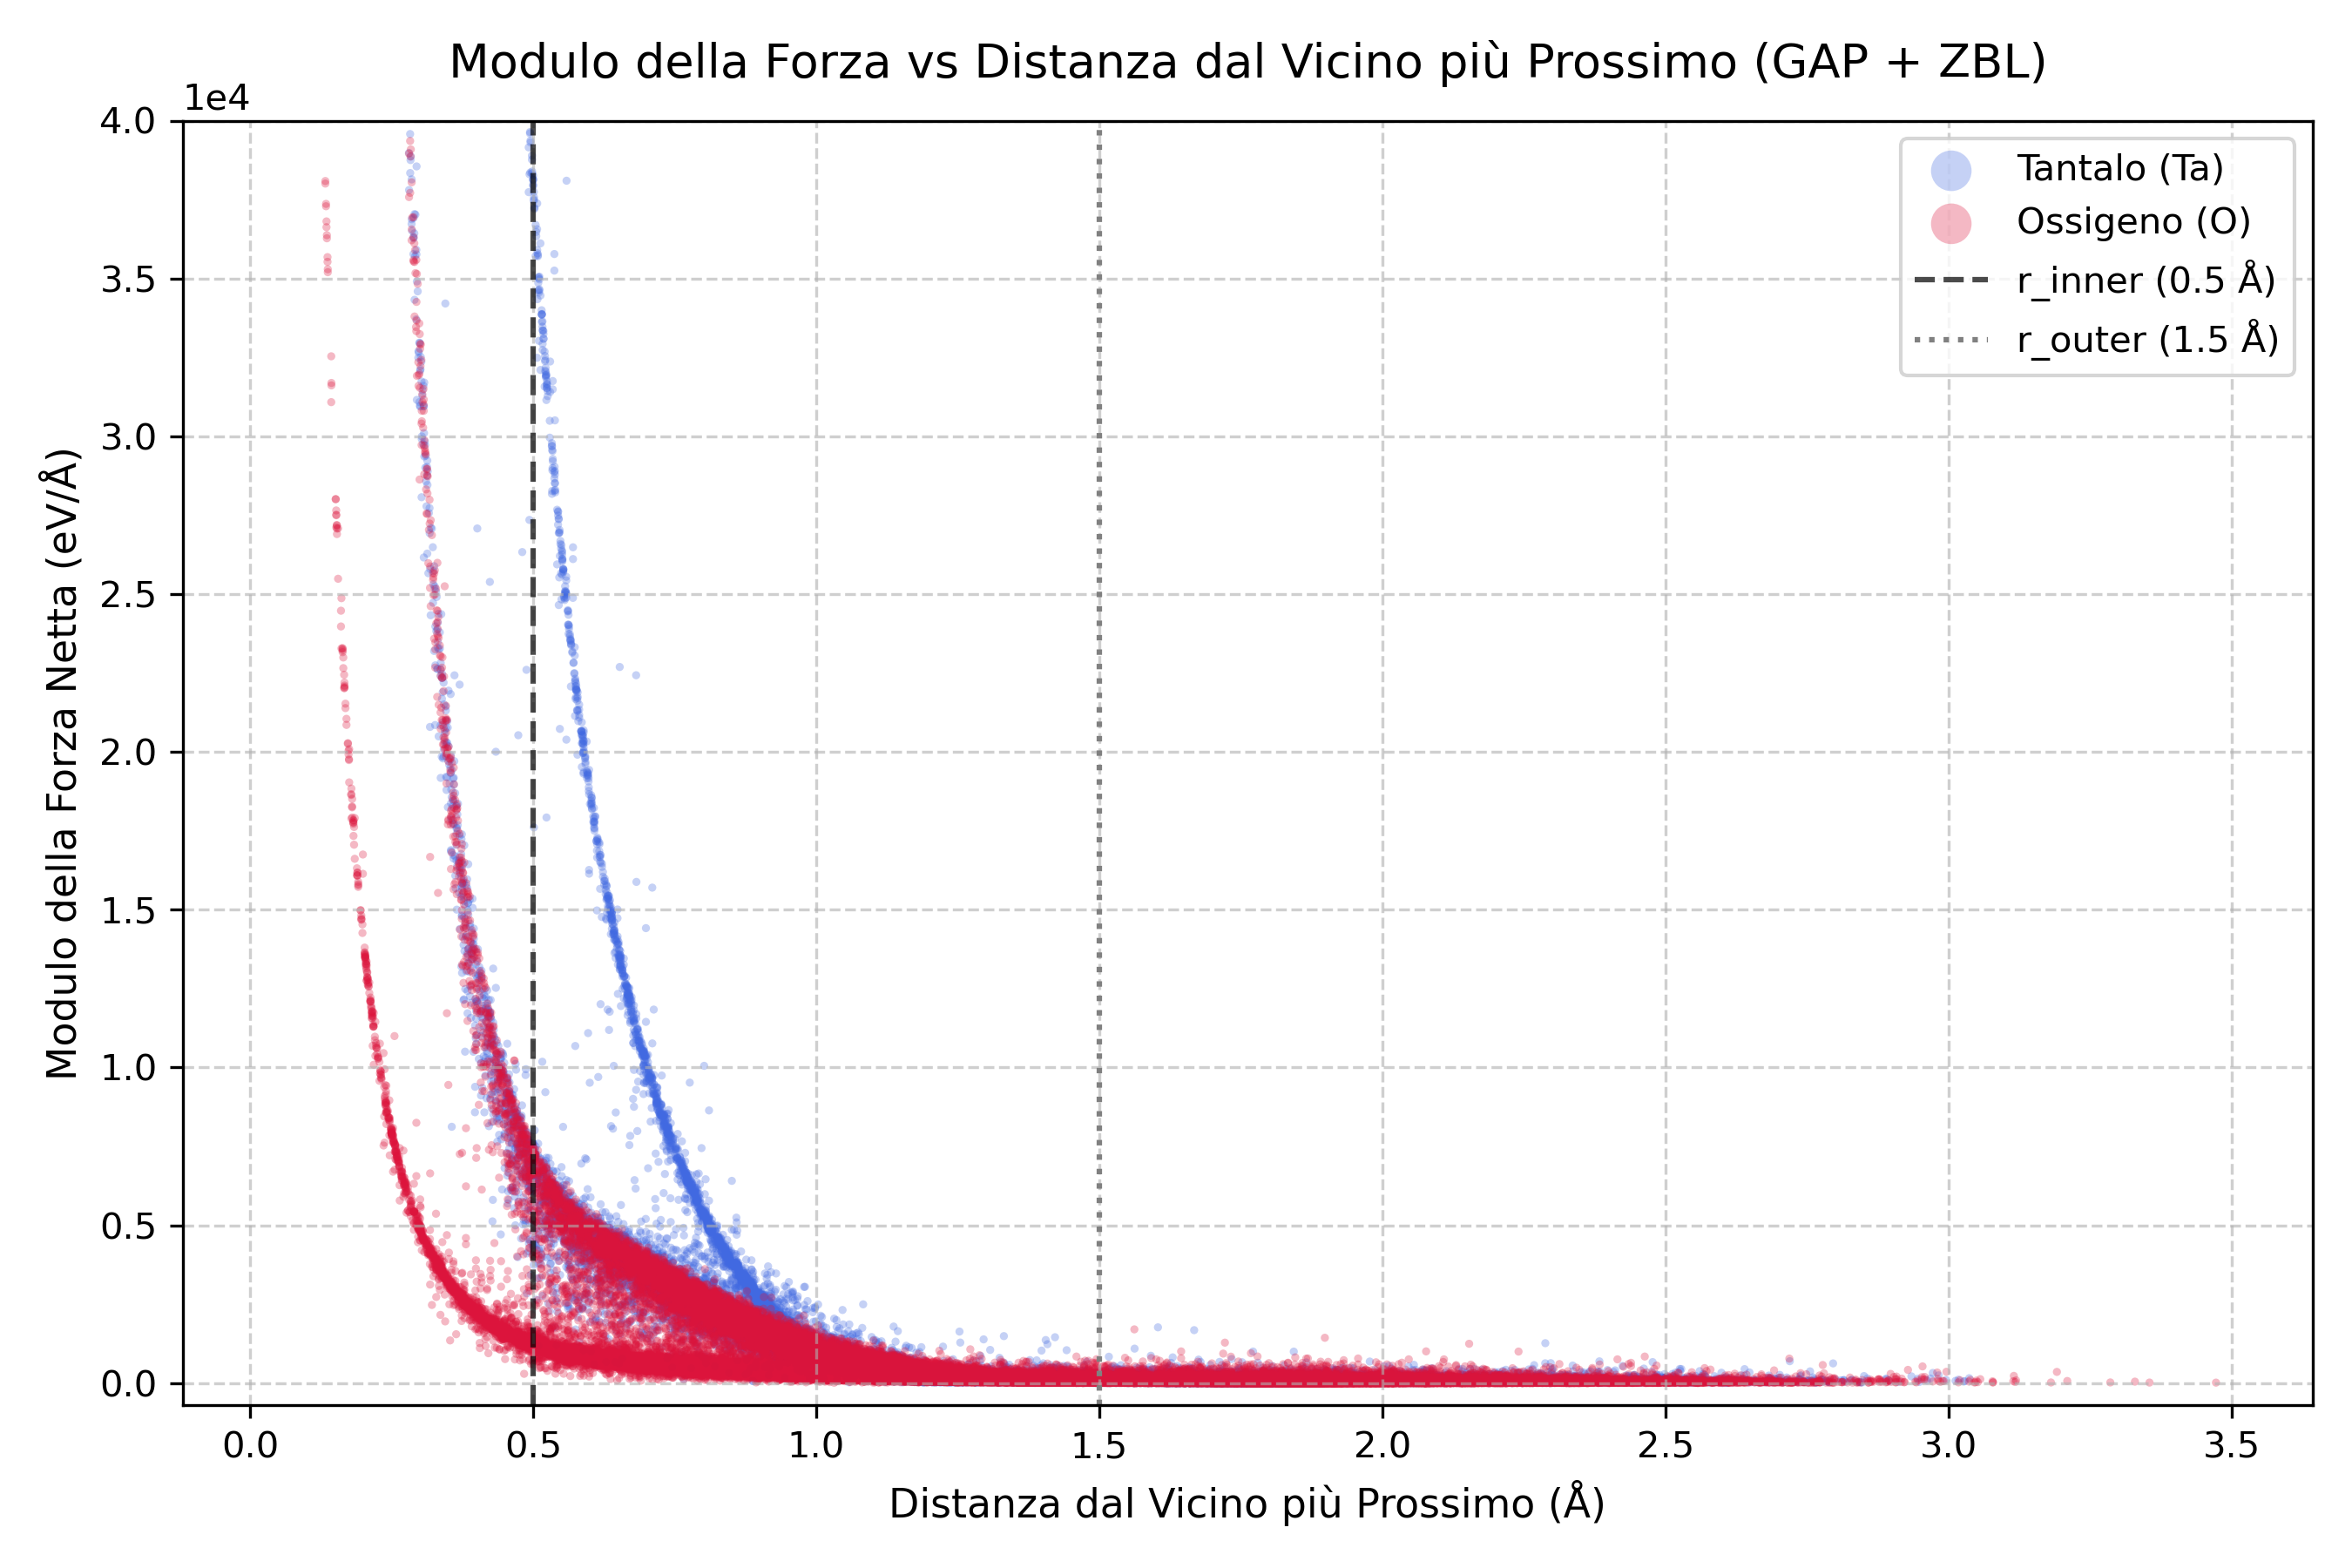
\includegraphics[scale=0.37]{./img/andamento_forze_totali_distanza_zbl.png}
        \caption{Relazione tra i valori di forza e distanza tra i primi vicini per il potenziale GAP + ZBL}
    \end{subfigure}

    \caption{Distanze e relazione forze-distanze per il potenziale GAP + ZBL, originariamente la scala del pannello (b) raggiungeva $10^7$, è stata modificata in modo da evidenziare la regione di interesse.}
    \label{fig:confronto_forze_distanze_zbl}
\end{figure}
}

In questo caso è anche utile guardare al confronto tra i due contributi di forza (\autoref{fig:confronto_forze_vs_distanza_minima_zbl}), osserviamo come i valori di distanza tra i primi vicini arrivino comunque sotto la soglia imposta come minima. Proponiamo come spiegazione di questo fenomeno il fatto che la correzione dello ZBL non sia adeguata a compensare i valori prodotti dal potenziale GAP, essendo questi molto distanti dalle configurazioni di training. Inoltre vogliamo far notare come i moduli delle forze a distanze piccole siano dati quasi totalmente dalla repulsione prodotta dallo ZBL, questo ci permette di confermare il suo comportamento adeguato. In conclusione non è immediatamente chiaro il motivo per il quale questa correzione non porti a risultati più in linea con le previsioni fatte.

\begin{figure}[h]
    \centering
    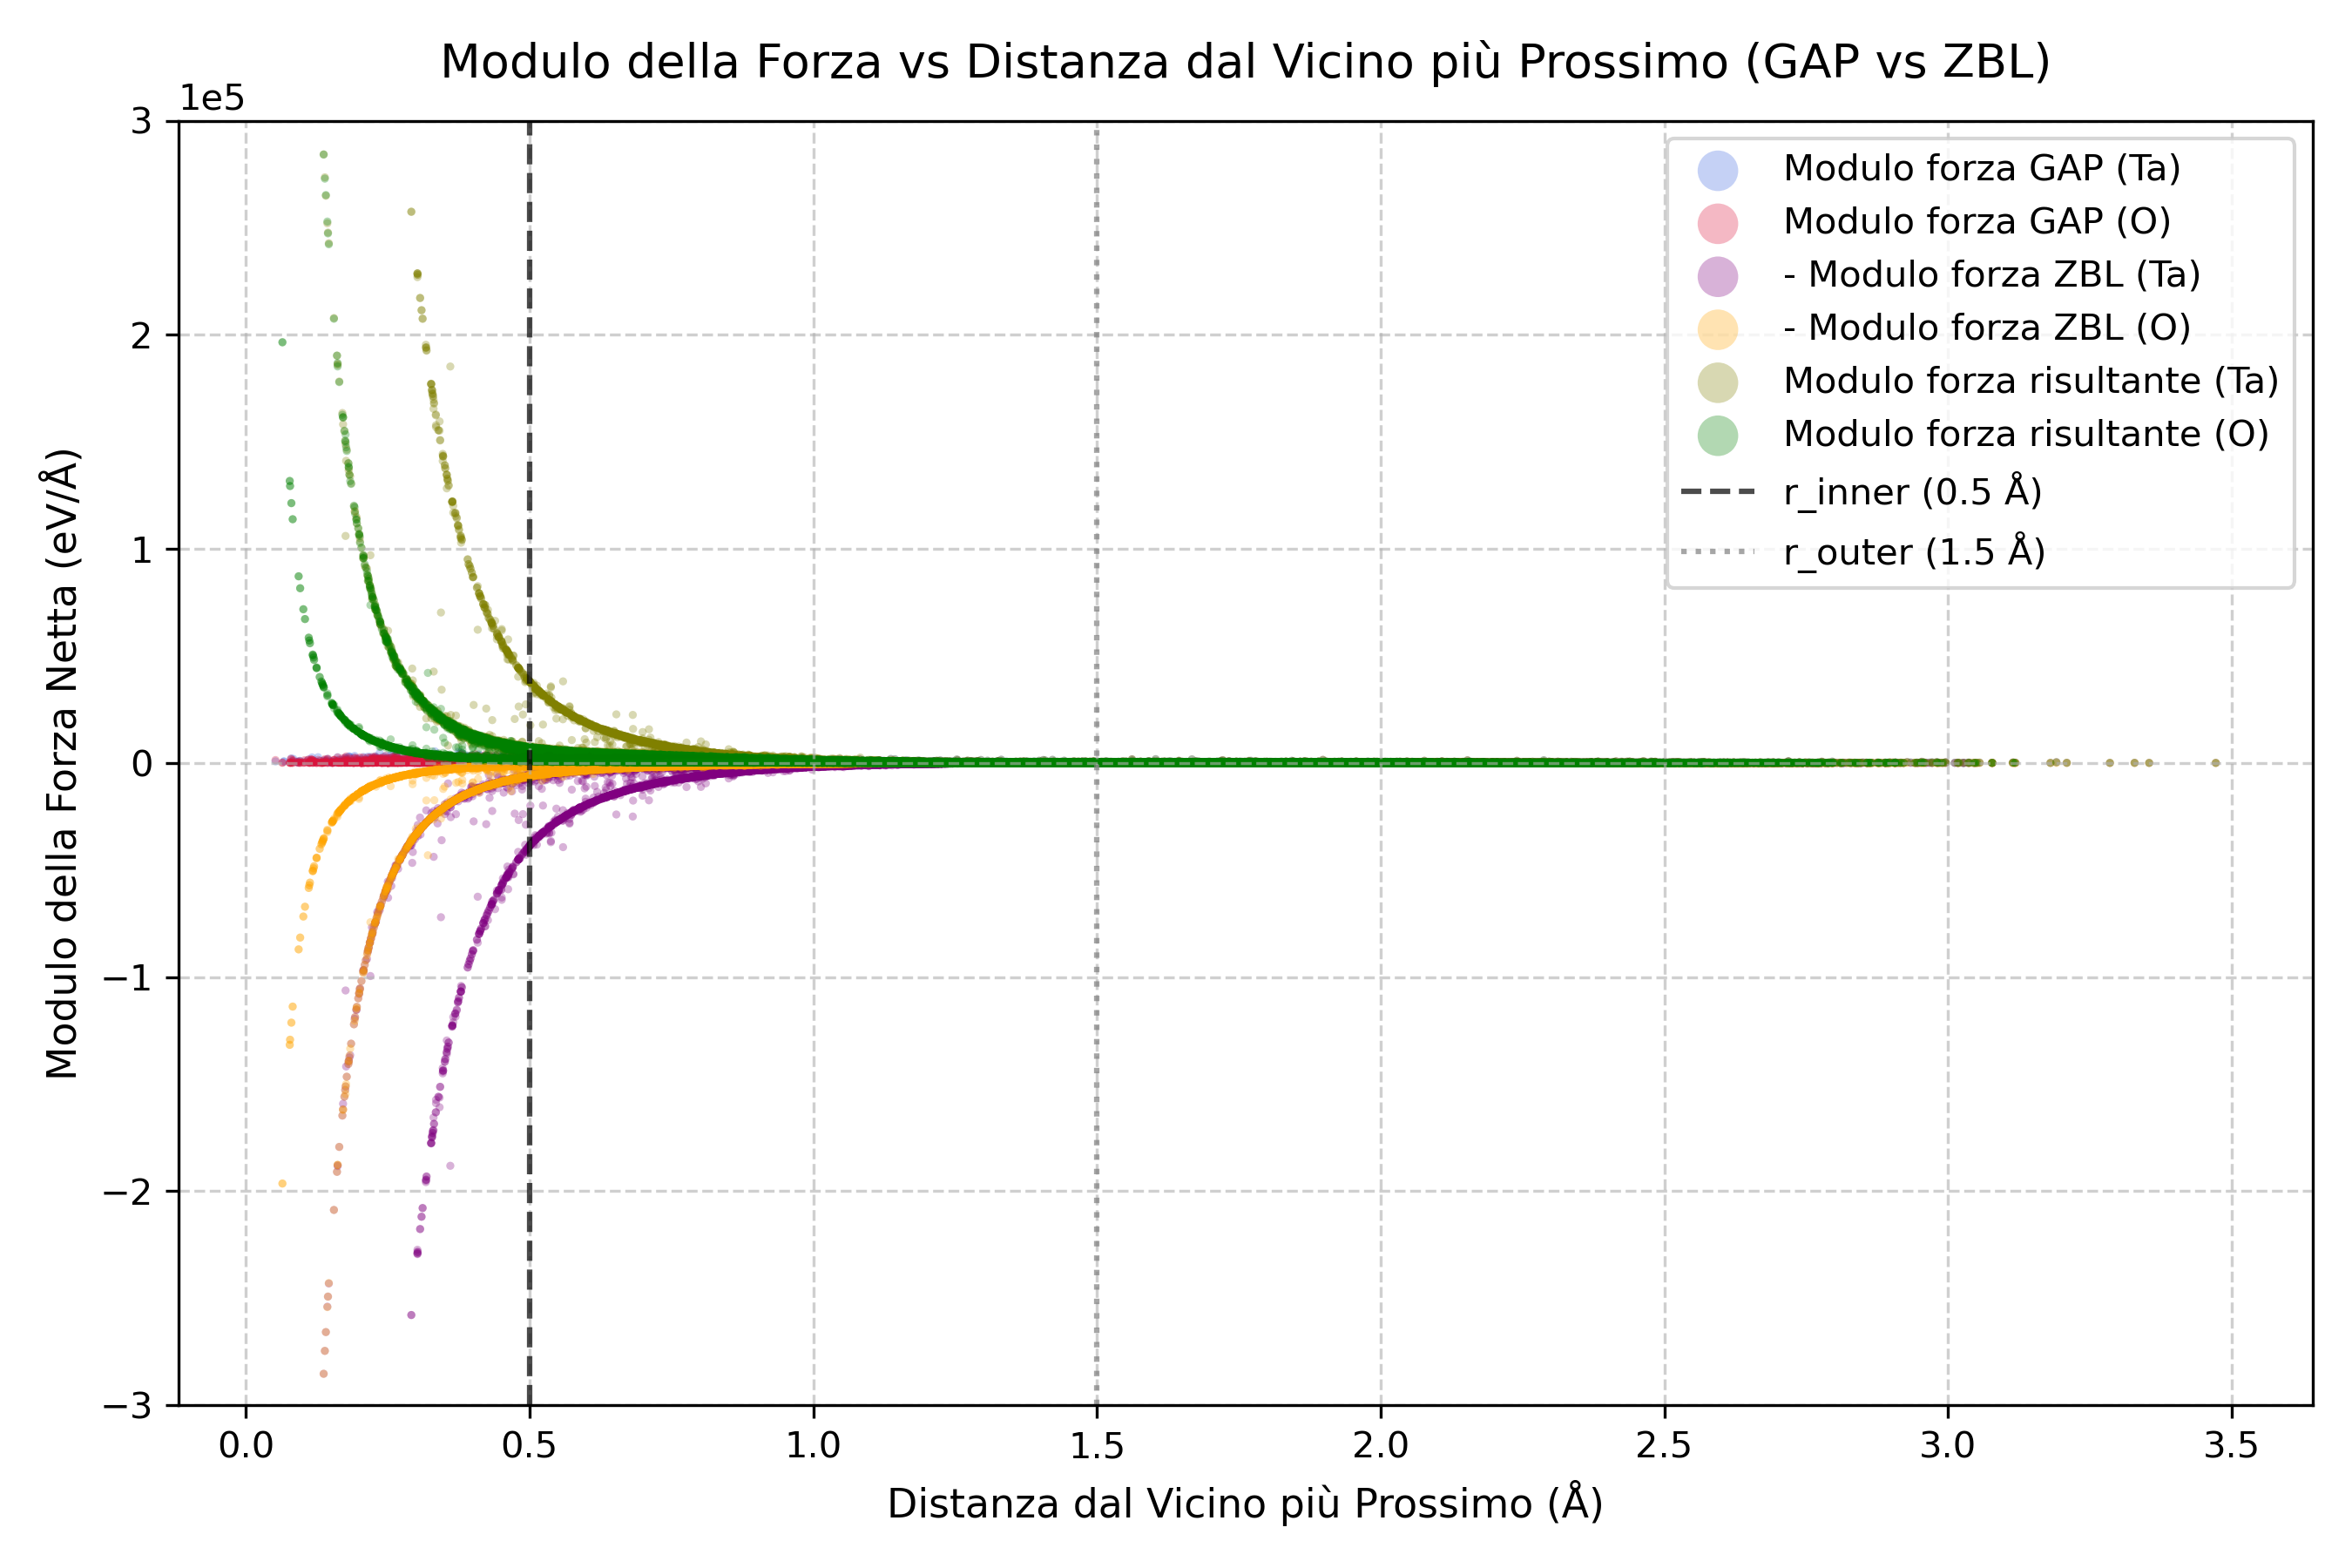
\includegraphics[scale=0.36]{./img/confronto_forze_vs_distanza_minima_zbl.png}
    \caption{Grafico del confronto tra i contributi di forza di GAP e di ZBL, la scala era originariamente fino a $10^7$, è stata ridotta in modo da evidenziare la parte di interesse.}
    \label{fig:confronto_forze_vs_distanza_minima_zbl}
\end{figure}

\section[Algoritmo di Metropolis]{Simulazione con metodo Monte Carlo e algoritmo di Metropolis}

Discutiamo adesso i risultati ottenuti tramite la simulazione Monte Carlo, vogliamo subito dire che non è presente una versione con il potenziale ZBL, in quanto, per costruzione, le distanze minime tra i vari atomi non scendono sotto i valori utilizzati nella sezione precedente.

Per questa simulazione abbiamo mosso un atomo per volta, entro un cubo di lato $0.01$ \AA, e abbiamo deciso di svolgere $80'000$ iterazioni, che equivalgono a $650$ Monte Carlo sweep, possiamo dire in questo modo che in media un atomo ha avuto $650$ possibilità di muoversi.

In questo caso l'unico grafico di energia che ha senso guardare è quello per l'energia potenziale (\autoref{fig:andamento_energia_montecarlo}):

\begin{figure}[h!]
    \centering
    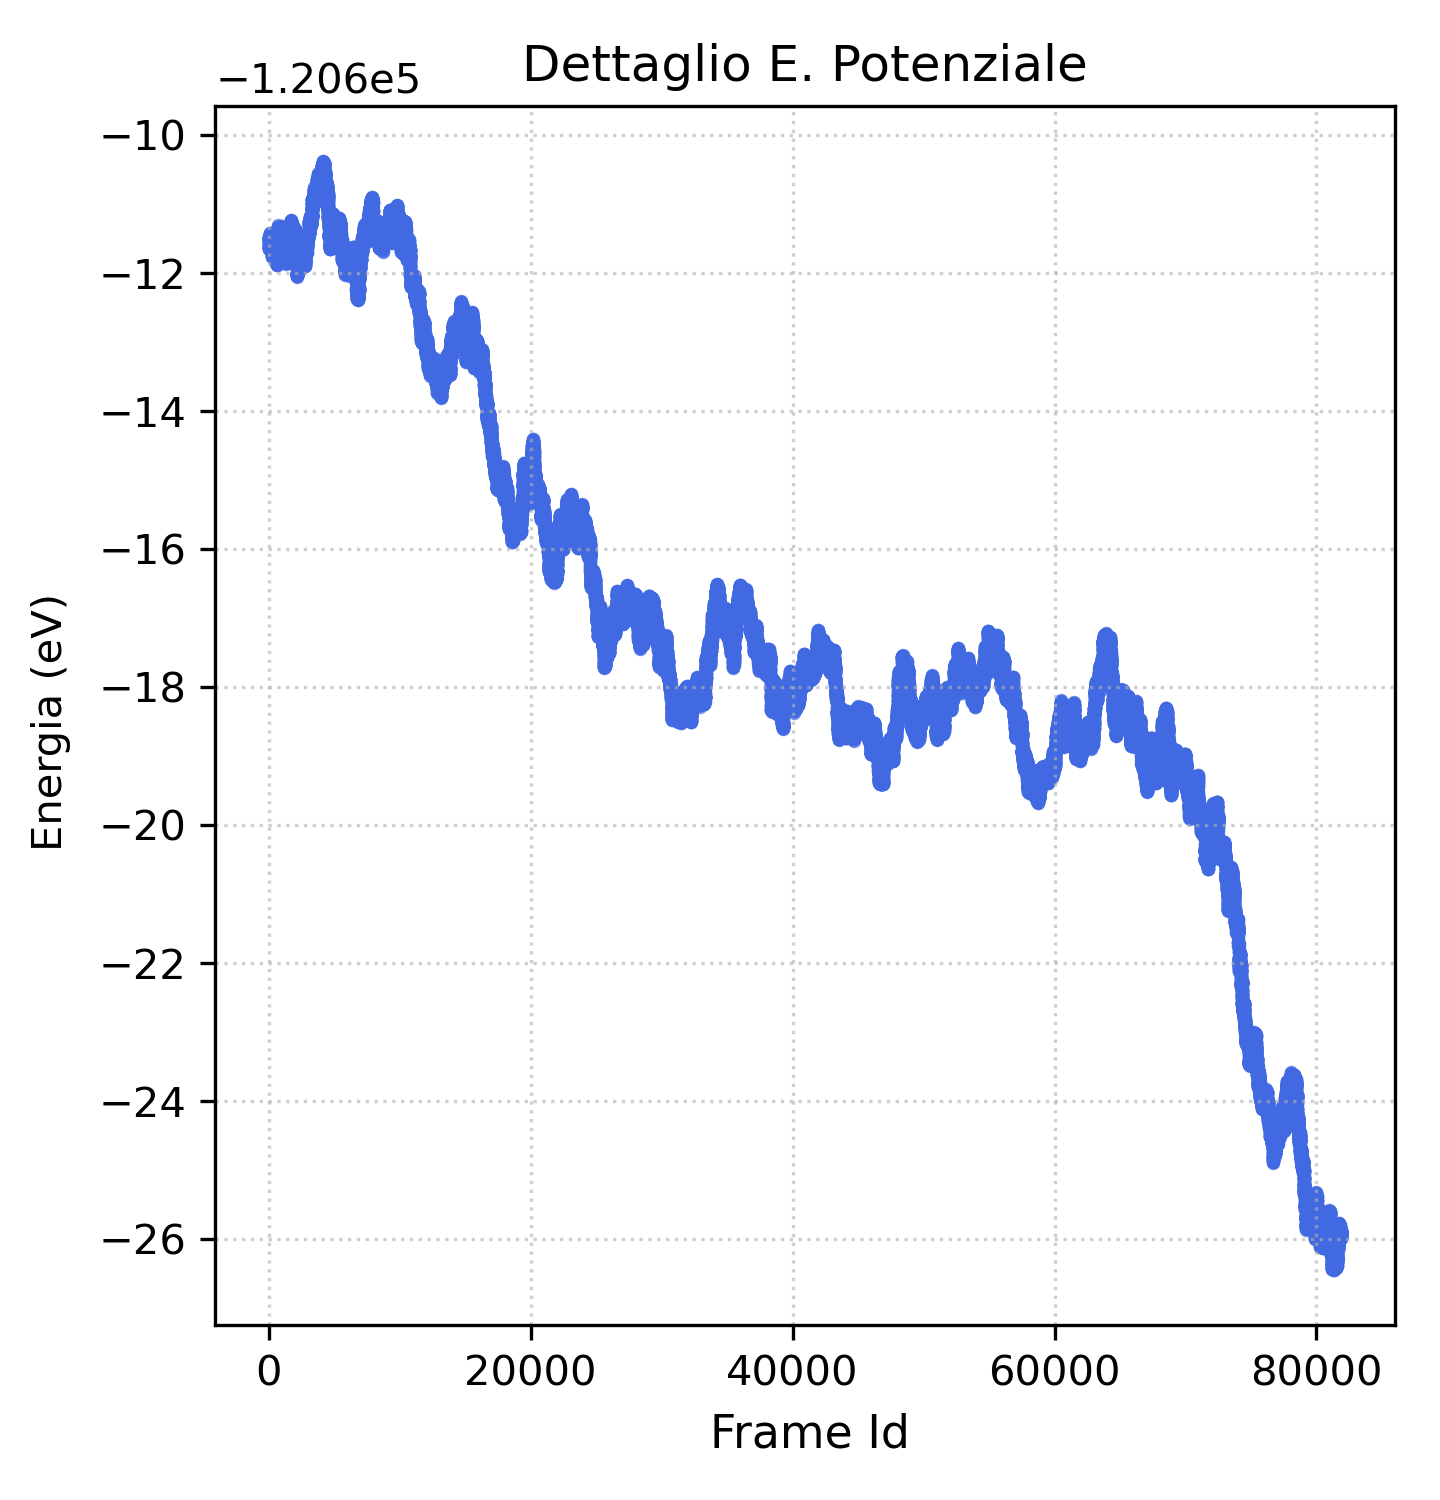
\includegraphics[scale=0.42]{./img/andamento_energia_montecarlo.png}
    \caption{Grafico dell'andamento in funzione dello step per i valori di energia potenziale}
    \label{fig:andamento_energia_montecarlo}
\end{figure}

notiamo che in questo caso i valori di energia rimangono stabili anche per molte iterazioni. Possiamo riconoscere ancora una tendenza a diminuire, ma in questo caso abbiamo anche sezioni in cui il valore oscilla senza un preciso trend.

Allo stesso modo abbiamo valori di forza che rimangono contenuti (\autoref{fig:andamento_forze_totali_montecarlo}).

\begin{figure}[h!]
    \centering
    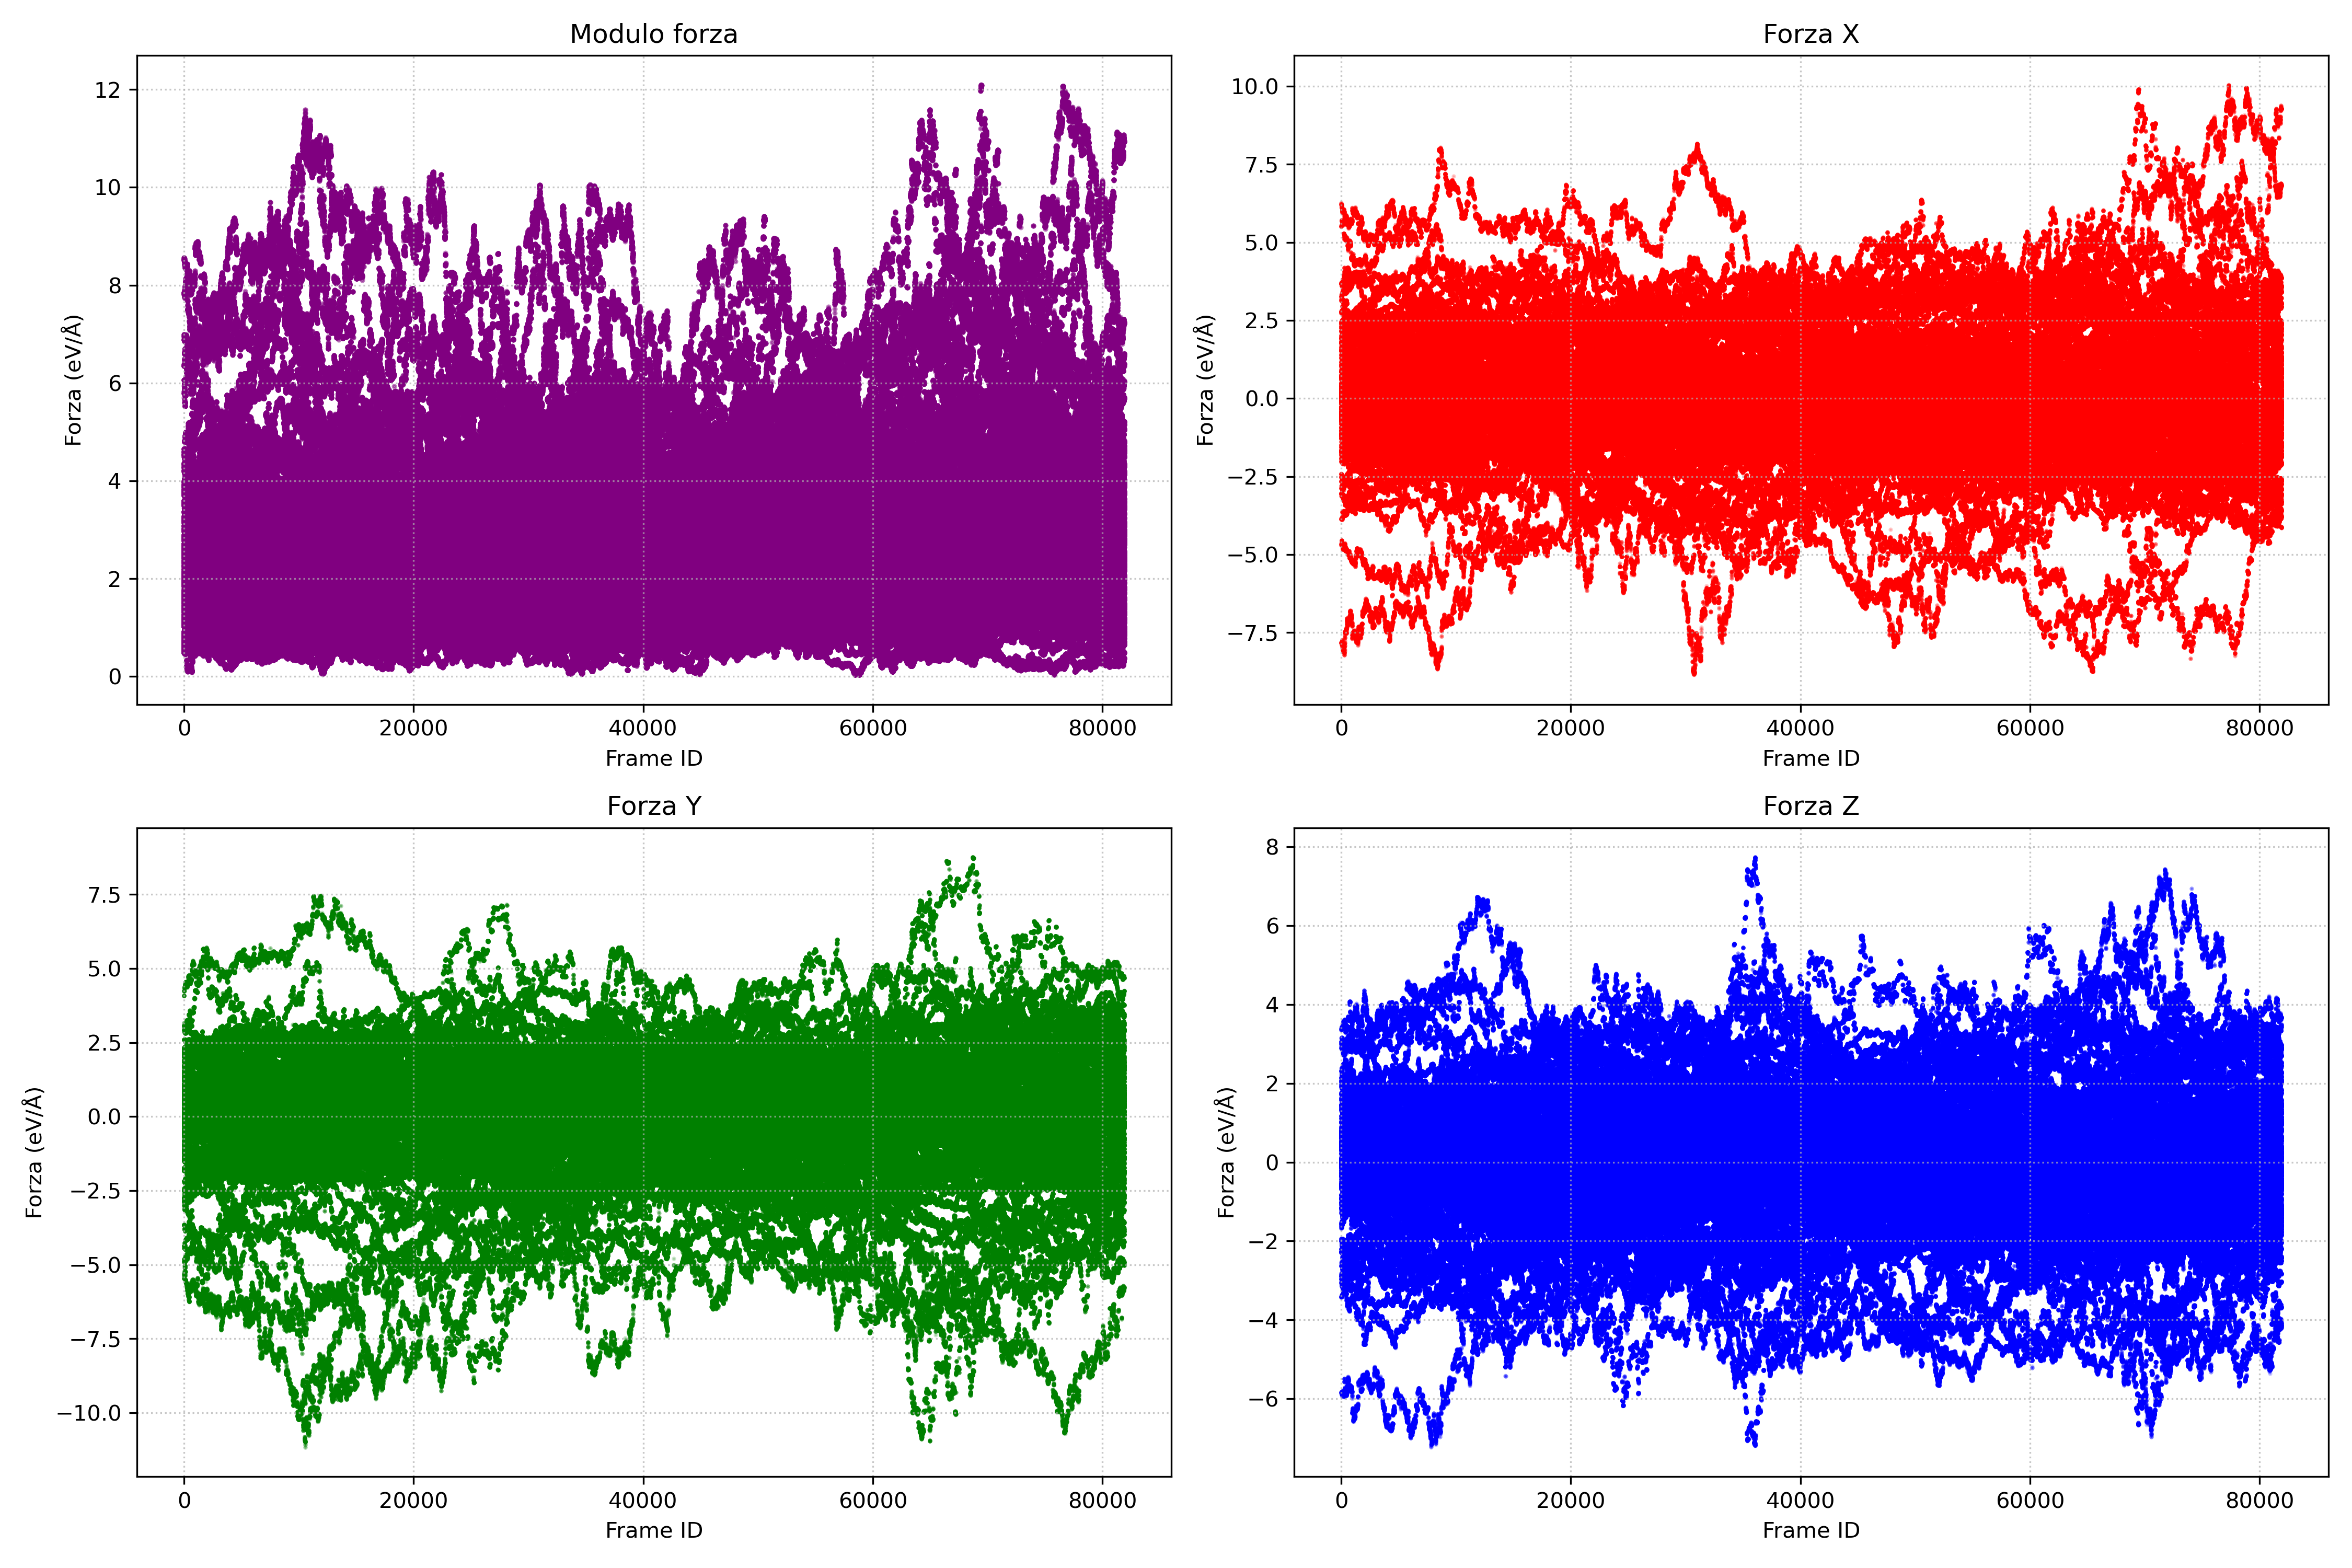
\includegraphics[scale=0.35]{./img/andamento_forze_totali_blocchi_montecarlo.png}
    \caption{Grafico dell'andamento in funzione dello step per i valori del modulo delle forze e relative componenti.}
    \label{fig:andamento_forze_totali_montecarlo}
\end{figure}

Come anticipato le distanze minime rimangono contenute e non degenerano verso zero, inoltre anche le forze in funzione della distanza minima presentano l'andamento che ci si aspetterebbe, come è possibile vedere in \autoref{fig:confronto_forze_distanze_montecarlo}.

{
\begin{figure}[ht]
    \centering

    \begin{subfigure}{0.48\textwidth}
        \centering
        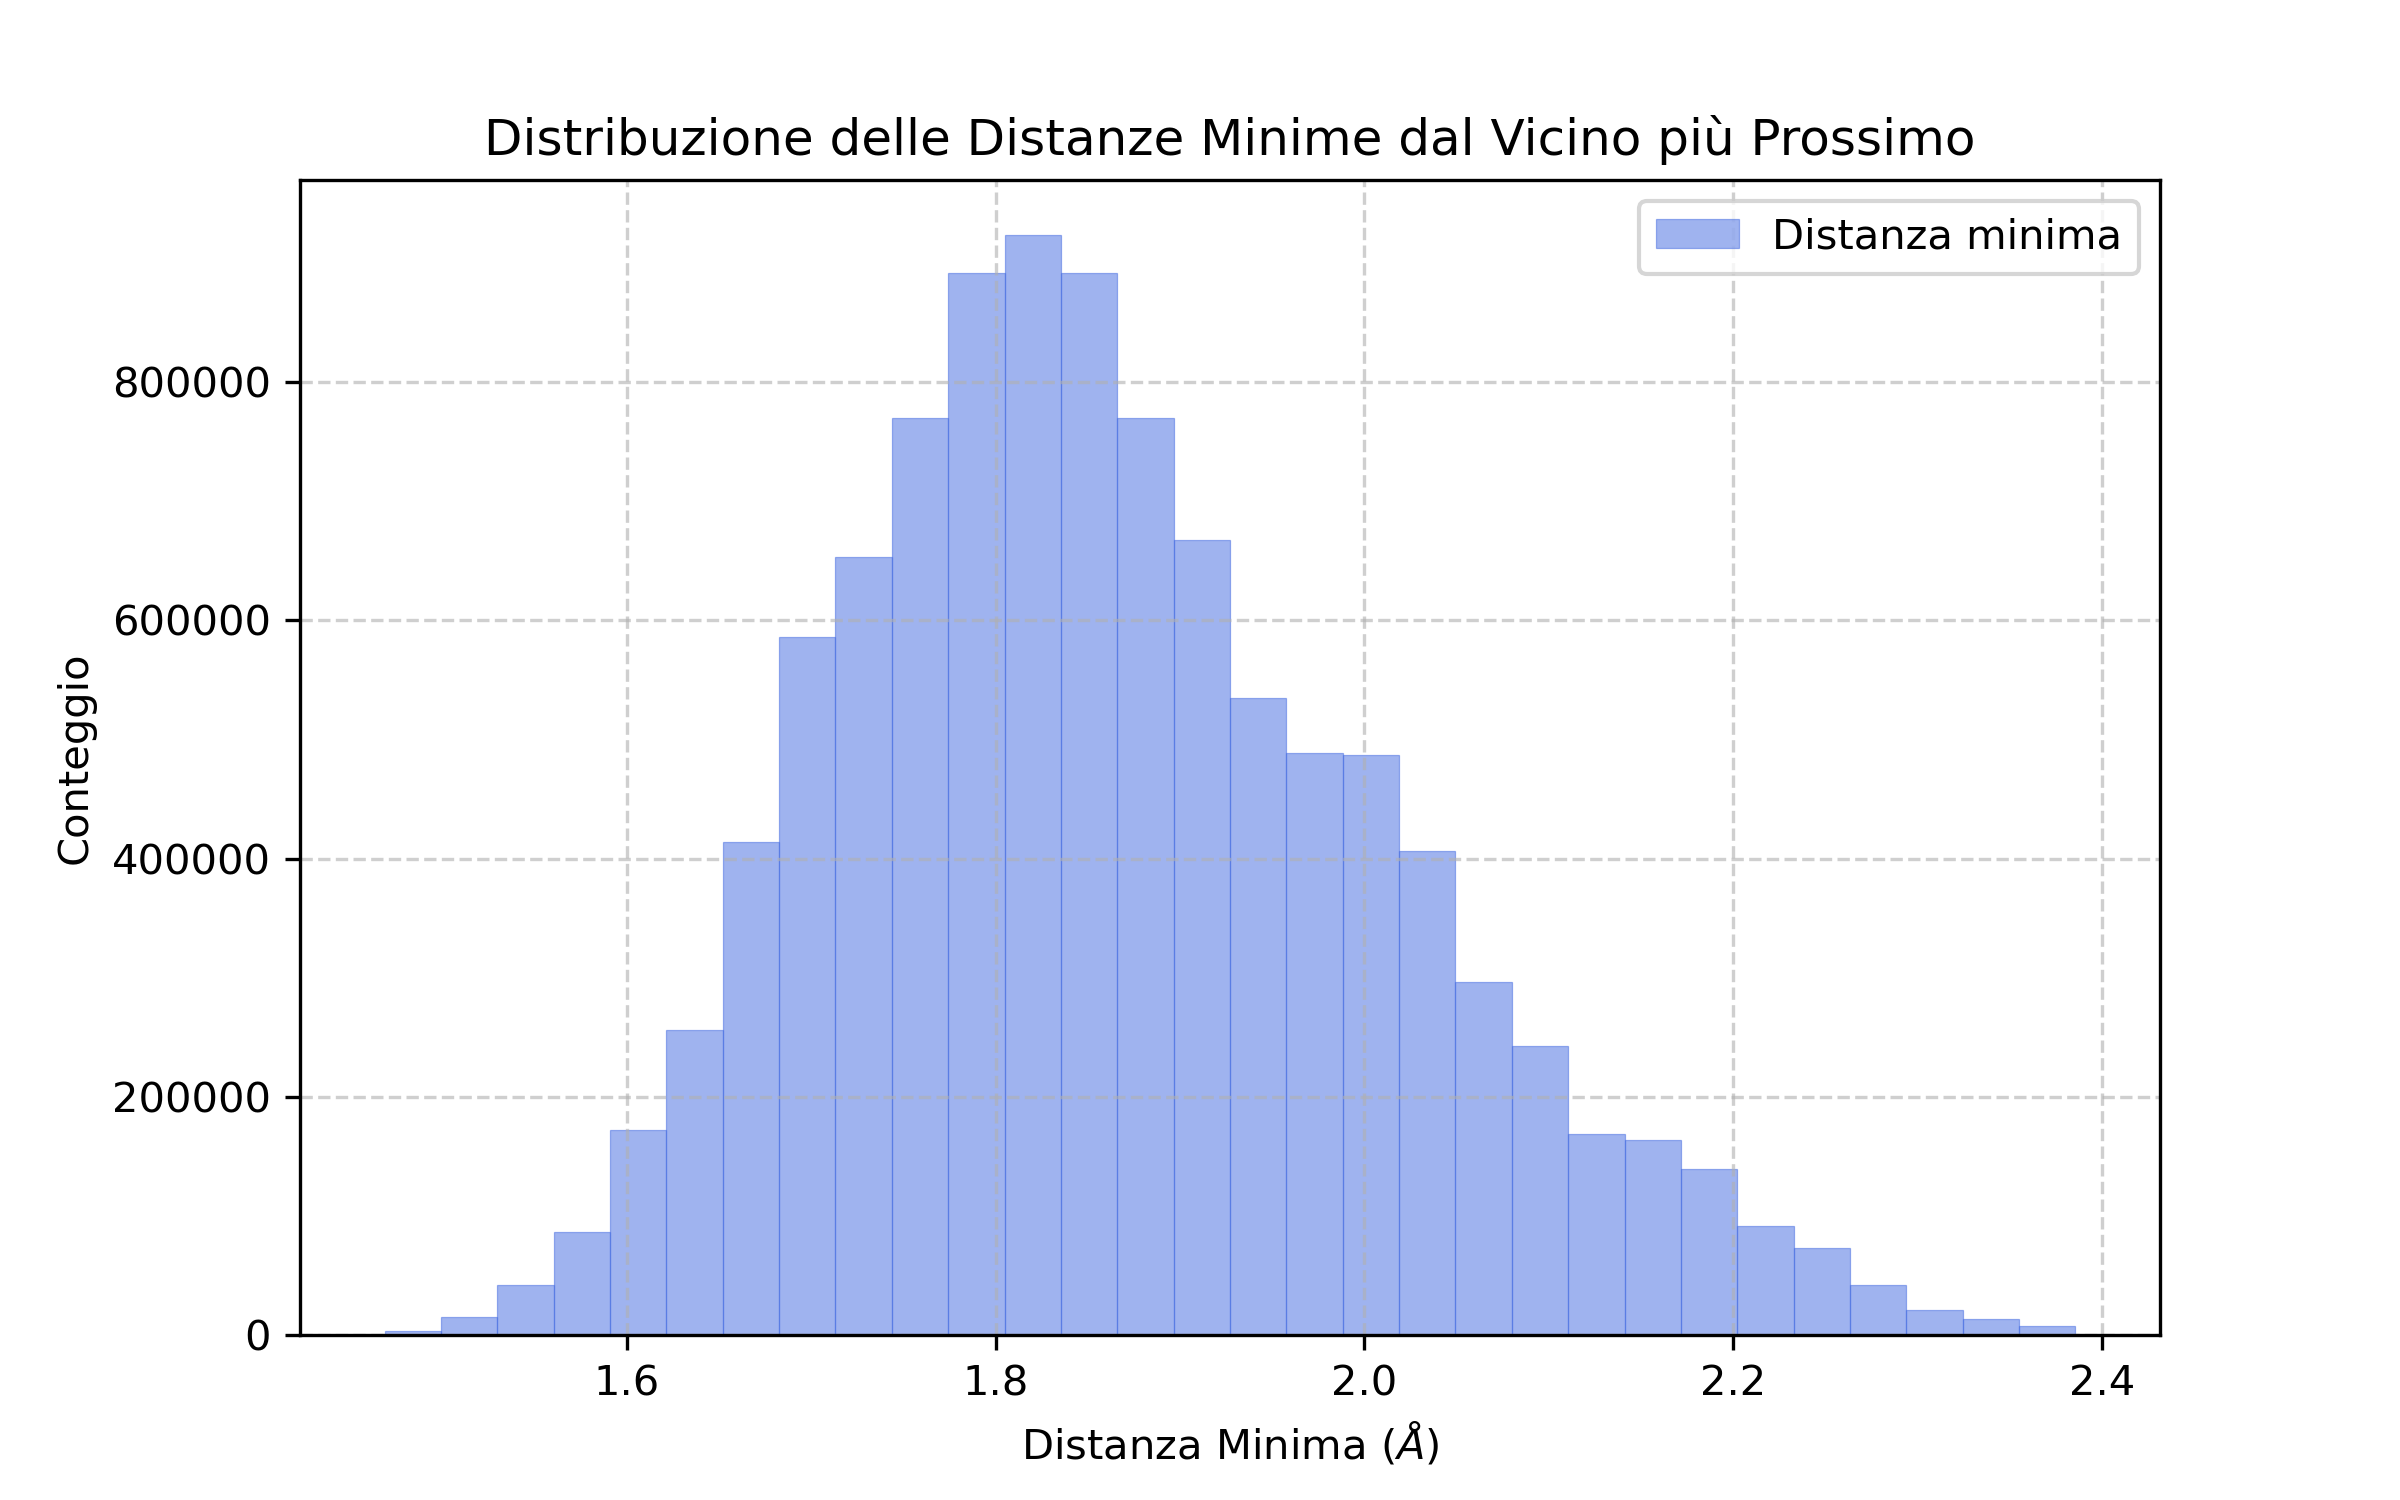
\includegraphics[scale=0.45]{./img/histo_distanze_montecarlo.png}
        \caption{Istogramma dei valori di distanza tra i primi vicini}
    \end{subfigure}
    \hfill
    \begin{subfigure}{0.48\textwidth}
        \centering
        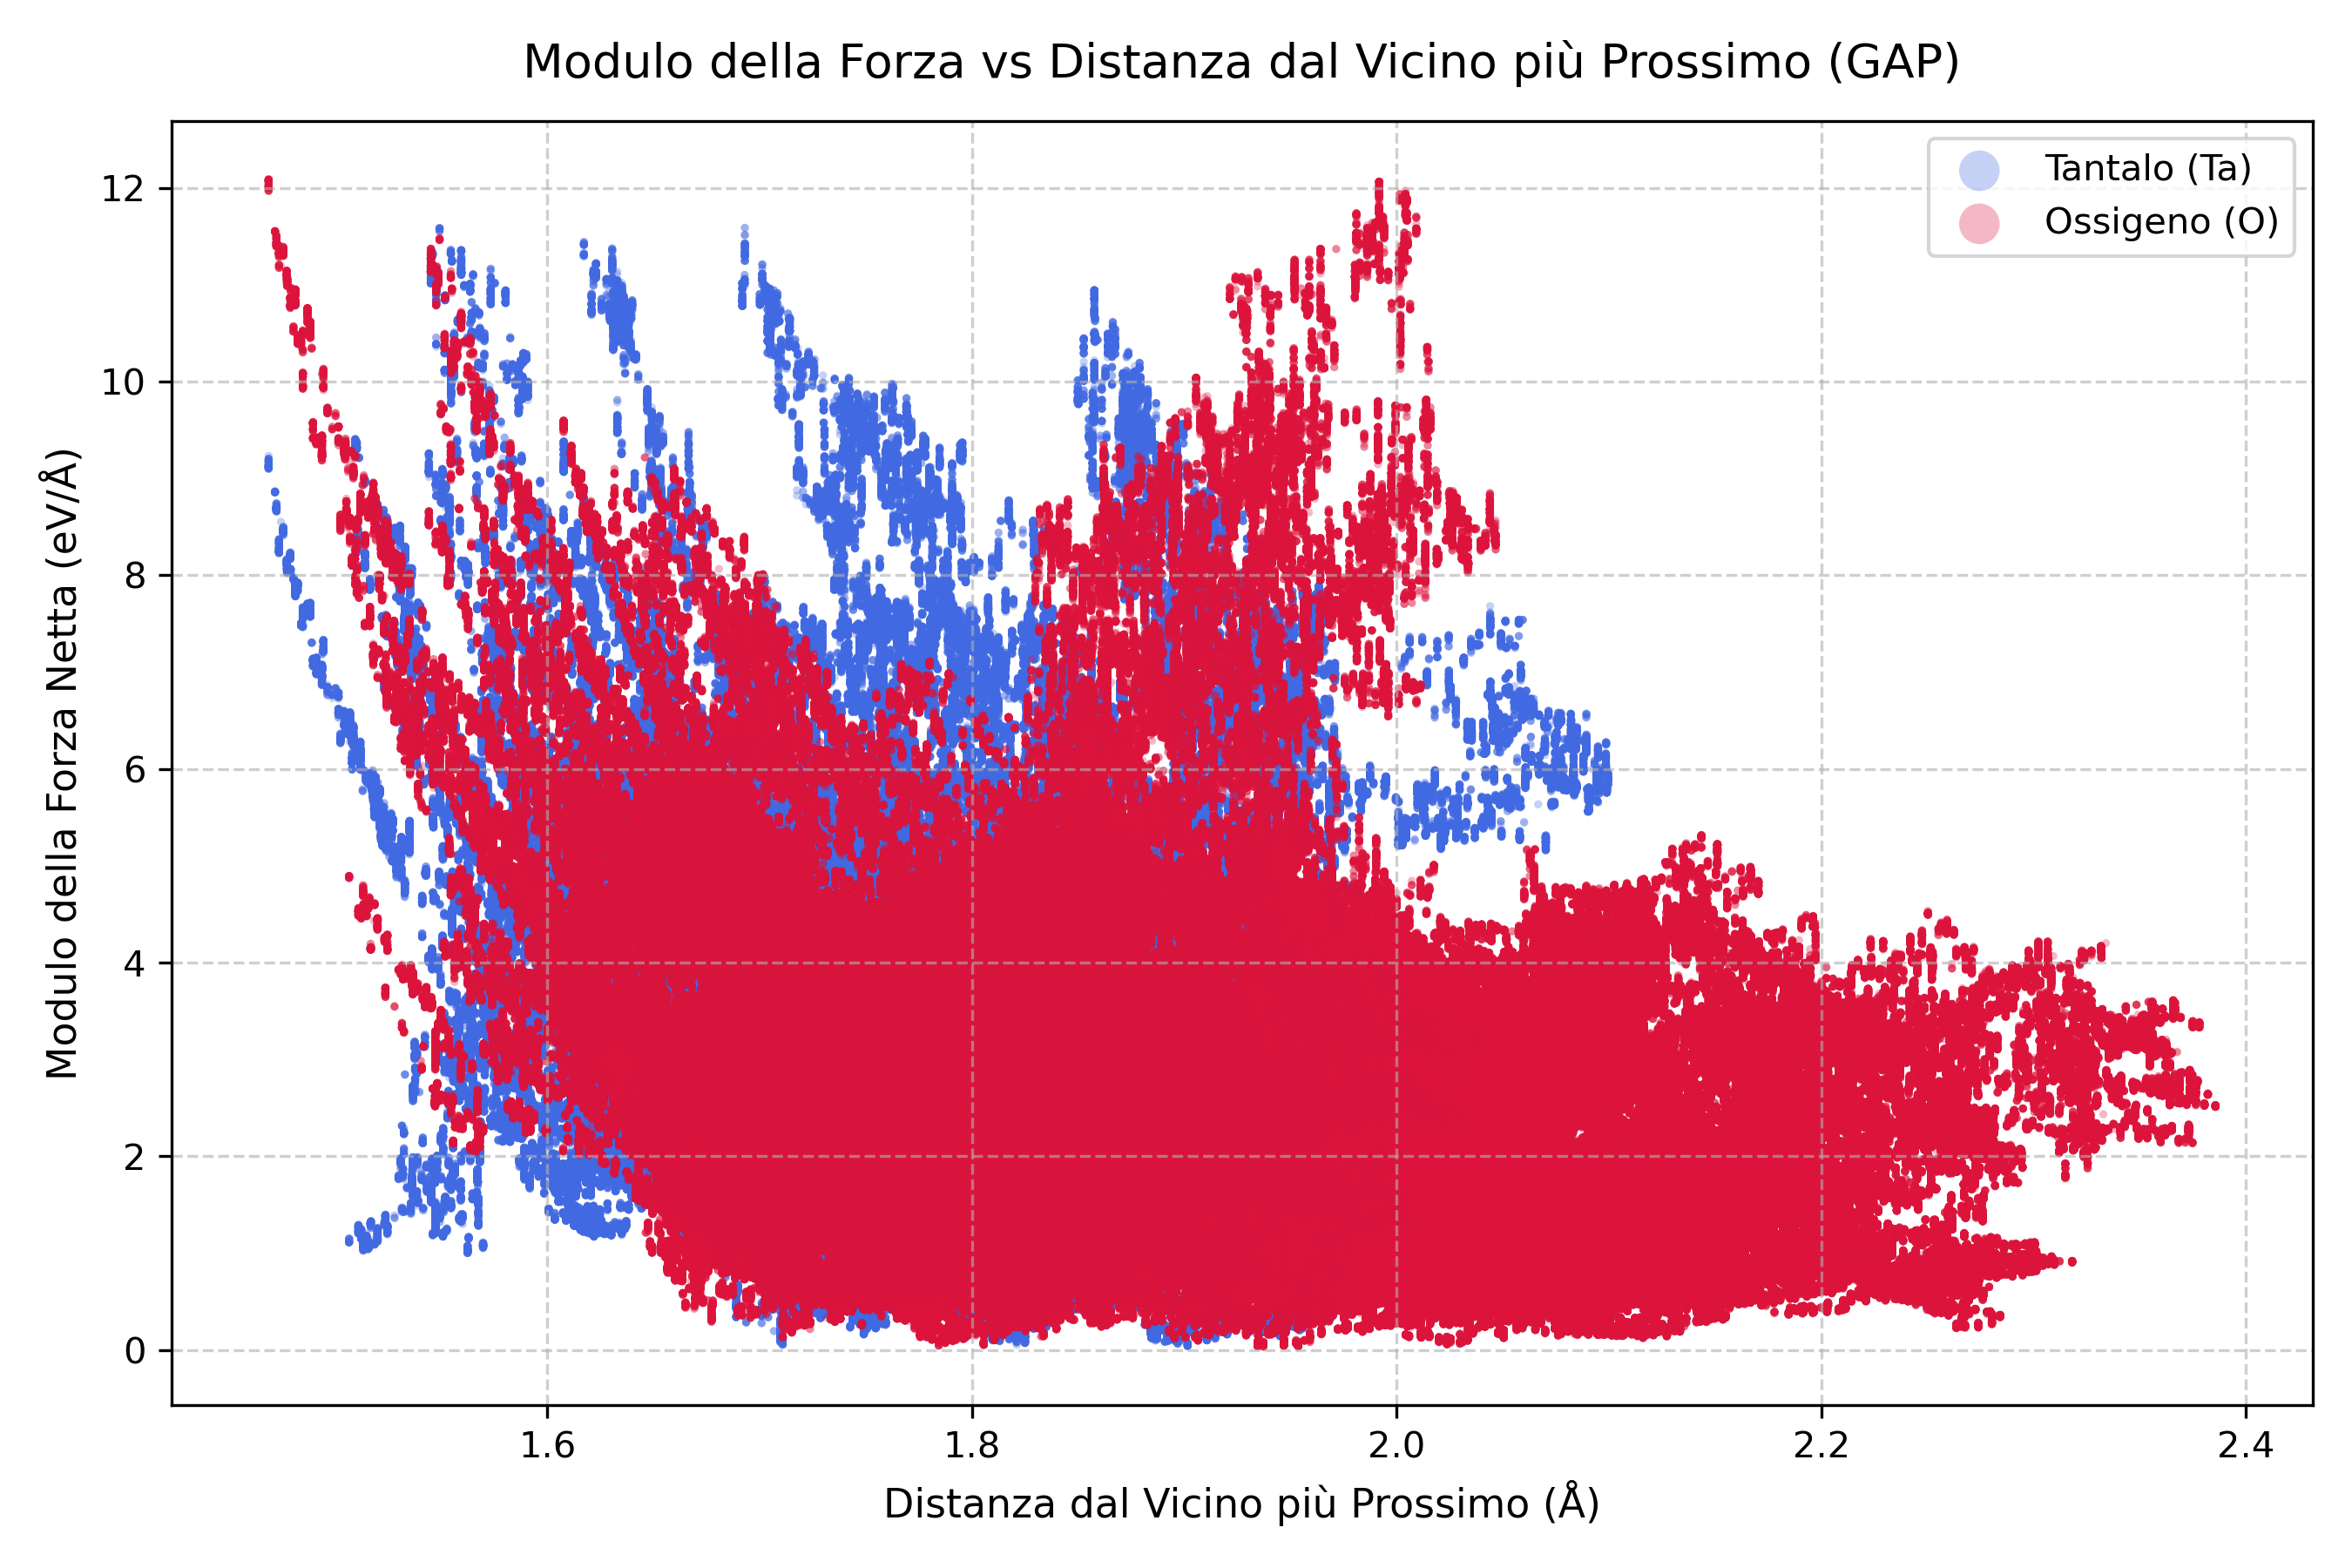
\includegraphics[scale=0.36]{./img/andamento_forze_totali_distanza_montecarlo.png}
        \caption{Relazione tra i valori di forza e distanza tra i primi vicini}
    \end{subfigure}

    \caption{Distanze e relazione forze-distanze per il potenziale GAP per la simulazione con algoritmo di Metropolis.}
    \label{fig:confronto_forze_distanze_montecarlo}
\end{figure}
}

%\clearpage

\section{Conclusioni}

In conclusione, possiamo dire che, è possibile utilizzare metodi di machine learning per velocizzare le simulazioni di materiali. È però fondamentale ricordare che essendo metodi di regressione non parametrici il risultato ottenibile, in fatto di range di configurazioni riproducibili, dipende fortemente dalle configurazioni utilizzate nella fase di training, oltre a questo, è anche fondamentale il descrittore che viene utilizzato per mappare l'ambiente che circonda un atomo. L'investimento computazionale iniziale usato per la fase di training, sotto le adeguate condizioni, permette di ottenere simulazioni sensibilmente più veloci.

\appendix %-------------------------------------------------------------------------

    \chapter[Dimensione del vettore di power spectrum]{Calcolo esplicito della dimensione del vettore di power spectrum}
\label{app:dimpowspec}

Non è immediato capire come siamo arrivati alla  formula \eqref{eq:formula-dimensione-semplificata}, conseguentemente diamo di seguito una spiegazione. Per prima cosa consideriamo il caso in cui $Z_1 = Z_2$, il più semplice e che usiamo come punto di partenza per la successiva generalizzazione.

Ci serve mantenere come riferimento equazione \eqref{eq:power-spectrum}, dove se si ha un solo $Z$ allora il numero finale di $p_{Z_1Z_2}(n,n',l)$ è dato solo da $n$, $n'$ e $l$. Per quanto riguarda $l$ ci sono esattamente $l_{max} + 1$ valori disponibili (in quanto si parte da zero), per capire come comportarsi con gli $n$, utilizziamo un piccolo aiuto grafico:

\begin{table}[h]
    \centering
    \begin{tabular}{c|cccc}
                 & $n_1$    & $n_2$    & $\cdots$ & $n_m$\\ \hline
        $n'_1$   &   11     &   12     & $\cdots$ & 1m\\ 
        $n'_2$   &   21     &   22     & $\cdots$ & 2m\\ 
        $\vdots$ & $\vdots$ & $\vdots$ & $\ddots$ & $\vdots$\\ 
        $n'_m$   &   m1     &   m2     & $\cdots$ & mm\\ 
    \end{tabular}
    \captionof{schema}{Struttura schematica per la combinazione dei valori di $n$ e $n'$ nel power spectrum}
    \label{sch:tabella-coefficienti-n-combinazione-power-spectrum}
\end{table}

dato che nel power spectrum gli $n$ compaiono in coefficienti che definiscono l'informazione strutturale, con $Z$ diversi, fanno riferimento a mappe di densità diverse. Inoltre ricordiamo che $n$ indica una sorta di distanza radiale. Questo significa che per il medesimo $Z$, la combinazione di $(n, n')$ produce lo stesso risultato di $(n', n)$ in quanto la mappa di densità è la medesima. Per diminuire la dimensione del vettore finale consideriamo solo gli elementi unici, ad esempio la parte triangolare superiore, ma allora il numero di elementi è la somma di $n_m$ elementi sulla prima riga, $n_m - 1$ sulla seconda e così via fino ad arrivare a un singolo elemento. Questo coincide con la somma dei primi $n_m$ numeri naturali, risolta da Gauss come:

\begin{equation}
    \mathrm{somma}(a) = \frac{a(a + 1)}{2}
    \label{eq:somma-gauss-naturali}
\end{equation}

Consideriamo adesso la presenza di un numero di specie maggiore di 1, allora dobbiamo considerare il fatto che lo scambio degli $n$ produce risultati diversi, in quanto fa riferimento a mappe di densità diverse. Le combinazioni di $Z$ (che sono simmetriche per lo scambio in quanto lo è il prodotto) si possono immaginare con uno schema identico a quello (\ref{sch:tabella-coefficienti-n-combinazione-power-spectrum}) dove, al posto di $n$ mettiamo i vari $Z$, da questo ricaviamo la seguente distinzione:

\begin{itemize}
    \item[-] $(Z_i,Z_i)$ gli elementi sulla diagonale, sono esattamente pari al numero di specie chimiche distinte presenti, ognuno di essi ha una combinazione di $n$ pari al numero definito in precedenza \eqref{eq:somma-gauss-naturali}
    
    \item[-] $(Z_i,Z_j)$ con $i \neq j$, questi per la simmetria già menzionata, sono esattamente gli elementi sul triangolo superiore meno quelli sulla diagonale. Possiamo facilmente vedere che questa somma si ottiene con la formula di Gauss \eqref{eq:somma-gauss-naturali}, dove adesso $a = S - 1$, con $S$ numero di specie presenti. Data la perdita di simmetria ognuna di queste coppie ha $n^2$ elementi distinti da tenere in considerazione
\end{itemize}

Se procediamo a mettere tutto assieme otteniamo la seguente espressione:

\begin{equation}
    \mathrm{dimensione} = (l_{max} + 1) \left( \frac{S\cdot n_{m}(n_m + 1)}{2} + \frac{S(S-1)n_m^2}{2} \right)
\end{equation}

che se andiamo a semplificare otteniamo l'espressione indicata in equazione \eqref{eq:formula-dimensione-semplificata}.

In conclusione, possiamo rappresentare l'insieme di questi coefficienti come un vettore, la cui dimensione è fissata e non dipende dall'input (quanti vicini / come è strutturato l'ambiente per un dato atomo) ma solo dai parametri che abbiamo utilizzato per descriverlo.



\backmatter %-----------------------------------------------------------------------
    
   \printbibliography
    
\end{document}
